\documentclass[english, LaM, oneside]{sapthesis}%remove "english" for a thesis written in Italian
%Bachelor's (laurea triennale) thesis : Lau 
%Master's (laurea specialistica) thesis: LaM 
%PhD's thesiss: PhD 
%\usepackage[italian]{babel} %use this package for a thesis written in Italian
\usepackage[utf8]{inputenx}
\usepackage{indentfirst}
\usepackage{microtype}

\usepackage{minted}
\newminted{python}{%
    % options to customize output of pythoncode
    % see section 5.3 Available options starting at page 16
}

%\usepackage{chemformula}
%\usepackage{setspace}
%\usepackage{yfonts,color}
%\usepackage{siunitx}
%\usepackage{comment}
%\usepackage{multirow}
%\usepackage{varioref}
%\usepackage[bottom]{footmisc}
%\usepackage{wrapfig}
%\usepackage{float}
%\usepackage{type1cm}
\usepackage{lettrine}
\linespread{0.9}
%\usepackage{chngcntr}
\usepackage[nottoc, notlof, notlot]{tocbibind}
%\onehalfspacing
%\counterwithout{footnote}{chapter}
\usepackage{hyperref}
\hypersetup{
			hyperfootnotes=true,			
			bookmarks=true,			
			colorlinks=true,
			linkcolor=red,
                        linktoc=page,
			anchorcolor=black,
			citecolor=red,
			urlcolor=blue,
			pdftitle={Evaluating continual learning strategies for audio classification},
			pdfauthor={Alessandro Taglieri},
			pdfkeywords={thesis, sapienza, roma, university}
 }

\title{Evaluating continual learning strategies \\for audio classification}
\author{Alessandro Taglieri}
\IDnumber{189094}
\course[]{Data Science}
\courseorganizer{Facolt\`a di Ingegneria dell'informazione, informatica e statistica}
\submitdate{2020/2021}
\copyyear{2021}
\advisor{Prof. Simone Scardapane}
\authoremail{taglieri.1890945@studenti.uniroma1.it}
\versiondate{\today}
\examdate{Something January 2022}

\begin{document}

\frontmatter
\maketitle

\dedication{To my beloved parents and brother}

\begin{abstract}
Continual learning generally refers to the algorithms which aim to learn continuously over time across varying domains, tasks or data distributions.
\newline \newline
One of the grand goals of Artificial Intelligence (AI) is building an artificial “continual learning” agent that constructs a sophisticated understanding of the world from its own experience through the autonomous incremental development of ever more complex knowledge and skills.  Current AI systems greatly suffer from the exposure to new data or environments which even slightly differ from the ones for which they have been trained for.
\newline \newline
In last years, many ideas that are also introduced in this thesis work, have been elaborated. This framework is becoming the most important focus on Deep Learning and many researches and studies have been done to optimize Artificial Intelligence, focusing on this field. A very important point of reference for my thesis work was all articles and works developed by \textit{ContinualAI} (\url{http://www.continualai.org/}) organization, supervised by \textit{Vincenzo Lomonaco}: an association that focuses all research and studies in Continual Learning scope.
\newline \newline
In this dissertation, we study the application of these ideas in light of the more recent advances in machine learning research and in the context of deep architectures for AI. We propose a comprehensive framework for the creation of different continual learning benchmarks on a new type of scope, never explored until now, based on Audio Classification. Moreover  substantial experimental evaluations of Continual Learning strategies on these benchmarks have been done with several consideration about that. All code for reproducing the experiments in this thesis as well as all testing on different CL strategies are available at \url{https://github.com/AlessandroTaglieri/thesis}.
\end{abstract}
\clearpage\null
\begin{acknowledgments}
\vspace{7mm}

\lettrine[lines=2, findent=3pt, nindent=0pt]{T}{}hroughout the writing of this dissertation I have received a great deal of support and assistance.
\newline \newline
I would first like to thank my supervisor, Professor Simone Scardapane, whose expertise was invaluable in formulating the research questions and methodology. Your insightful and continual feedback pushed me to sharpen my thinking and brought my work to an higher level.  I would like to thank you, also on a human level, for having made me passionate about a research field that was unknown until now and on which I hope I will be able to deepen my research and works in the future.
\newline \newline
I would like to express my deepest gratitude to Prof. Vincenzo Lomonaco, Assistant Professor at the University of Pisa and Co-Founding President of ContinualAI. His advice and his course on Continual Learning that I have attend in this period, have been very useful to complete and refine my thesis work. 
\newline \newline
I would like to thank my colleagues in this Master's degree during these two strange and not easy years, with whom I have collaborated on numerous projects and who have made me grow from all points of view, humanly and as a student.
\newline \newline
I am extremely thankful to my company where I work, Sistemi Informativi and all \textit{IBM Italy} through which I grew as a Data Scientist in parallel with my course of study. My colleagues, Valerio and Manuele, were essential with their precious advice and support during last three years. My work experience has been very stimulating in order to reach my goal to finish my studies with this Master program on time.
\newline \newline
Some special words of gratitude go to my friends who have always been a major source of support when things would get a bit discouraging: Riccardo A., Marco L., Stefano G.,Francesco A. . Thanks guys for always being there for me. The time to be together will never be too much. \newline
Thank you also my friends who are here this greateful day to celebrate this important milestone with me: Angelo D.B., Antonio S., Alessandro C., etc.. .
\newline
A special thanks to Riccardo D.P., besides being a lifelong friend, you have constantly helped me to settle in Sapienza; your advice and your support has been fundamental to reach this goal.
\newline \newline
My deep and sincere gratitude to my family for their continuous and unparalleled love, help and support: my uncles and my cousins, especially my grandmother \textit{Nonna Rita}, that helps and spoils me with her love and food.  My gratefulness also for my grandparents that are not physically here; you are always with me, in my hearth. A piece of this thesis is also for you!
\newline \newline
A simple thank you would not be enough to express my gratitude to a special person, my girlfriend Gloria. You are my strength, my  courage, my support in all moments of weakness. You have always been the first person to believe in me, through your tenacity, persistence and pure love. These two years were very long, not very easy and full of sacrifices; your presence at my side was essential, thank you.  
This milestone is one of the many goals that we will achieve together, side by side. 
\newline \newline
I am forever indebted to my parents for giving me the opportunities and experiences that have made me who I am. They selflessly encouraged me to explore new directions in life and seek my own destiny. My mom \textit{Paola} and my dad \textit{Patrizio}, your continued support and encouragement were essential in these two years. I can't forget my one and only loving big brother \textit{Andrea}; he is and will be my main point of reference for all features of my life.  
This journey would not have been possible if not for them, and I dedicate this milestone to them. 

\end{acknowledgments}
\clearpage\null
\tableofcontents

\mainmatter


\chapter{Introduction}
\section{Deep Learning}
We are living in the big data era where all areas of science and industry generate massive amounts of data. This concept has been around for years; most organizations now understand that with all the available data that they can collect from their businesses, they can applies analysis and get significant value and effort from it. Consequently we find ourselves in a situation with unprecedented challenges regarding their analysis and interpretation. For this reason, we should  take advantage of these data introducing new machine learning and AI methods. Nowadays Deep Learning is new methodology that receive much attention \cite{Hinton-2006}. It can be considered as an evaluation of machine learning; i.e. an evolution in the utilization of the data.
\newline \newline
Machine learning, with the introduction of the deep neural networks, has significantly improved the state of the art in solving many research and industrial problems. In a very large scale of scope, deep learning has introduced an evaluation: in vision problems there is an improvement of the state of the art in classification and detection, in natural language processing (\textit{nlp}) neural networks are used for search engine or text analysis and finally we got an improvement also in reinforcement learning performances.
\\
Deep learning allows computational models that are composed of multiple processing layers to learn representations of data with multiple levels of abstraction. These methods have improved a several field where AI is the main actor: speech recognition, visual object recognition, object detection and many other domains such as drug discovery and genomics \cite{deep-learning}. This technique is very useful when we work with large amount of data by using backpropagation algorithm that allow machine to change and optimize its internal parameters that are used to calculate the representation in every layer from the representation in the previous one.There are two main type of these methods:  Deep convolutional nets have brought innovation in several field, like processing video, speech, images and audio while recurrent nets improved the researching on sequential data such as text and speech.
\newline \newline
There are various fields where deep learning is the leading actor; just think to simple mobile apps that allow to recognize different type of images or sounds, robotics that can simulate human behaviors, self-driving cars, virtual vocal and chat bot that increase the customer experience for several organizations. Nowadays Artificial Intelligence is the integral part of every human life.
\newline \newline
A formal definition and a properly focusing on deep learning theory has been done in \hyperref[nn]{Chapter~\ref*{nn}}.


\section{From deep learning to continual learning}
Humans have the extraordinary ability to learn continually from experience. It's a fundamental aspect in everyday life, applying previously learned knowledge and skills to new situations. One of the most goal of AI is to build a continual learning paradigm that allows to implement a way to learn from own previous experience through ever more complex skills  \cite{ring}.
\newline \newline
However, the learning algorithms suffer from many shortcomings. An important disadvantage of deep learning is the strictly dependence on the quality of the data, it's needed to have a clean and well-built dataset to get a good learning process. In most machine learning algorithms, training data are assumed to be independent and identically distributed (iid), i.e. the data distribution is assumed static. If the data distribution changes while learning, the new data will interfere with current knowledge and erase it. This phenomenon is so important and it so drastically challenges the algorithms’ performance that we call it “\textit{catastrophic forgetting}” \cite{cat_forgetting}. This problem has many implications in the way algorithms train neural networks and in the potential application fields for machine learning.
Let us consider, for example, a robot working in an evolving environment and being assigned the goal of manipulating new objects or solving new tasks. The robot will then need to incrementally learn new knowledge and skills to improve and adapt its behaviour to new situations. With classical machine learning techniques, in order to incorporate new knowledge while avoiding catastrophic forgetting, the model will have to re-learn everything from scratch. A robot which needs only the new data to improve and develop knowledge and skills, would be much more efficient in this situation.
\newline \newline
However, artificial learning systems today seems very far from that goal. While during the last few years we have formidable progress in the context of semi-supervised and reinforcement learning (i.e. being able to operate with less and less direct supervision) with the ability to learn more autonomously \cite{goodfellow, lecun}, very little has been done in deep learning with the idea of learning continuously.
\newline \newline
Continual learning (CL) is a branch of machine learning aiming at handling this type of situation and more generally, settings with non-iid data sources. It aims at creating machine learning algorithms able to accumulate a set of knowledge learned sequentially. The general idea behind continual learning is to make algorithms able to learn from a real-life data source. In a natural phenomenon, the learning slots are not at the same time available and need to be handle sequentially. Learning from the present data and being able to continue later with new data rather than learning only once for all, seems very appropriate. It opens the possibility to improve the algorithms on a certain task or to make them learn new skills/knowledge without forgetting. It also enables transfer between learning experiences. Previous knowledge acquired may help in learning to solve new problems and new knowledge which may improve the solutions found for past tasks. Nevertheless, because of the catastrophic forgetting phenomena, learning continually is a challenging discipline. The method consisting in storing everything to avoid any forgetting is not enough because it would not be scalable about memory and computation. The amount of memory used might grow too fast. It is therefore important to remember only the essential concepts. Moreover, to deal with catastrophic forgetting, algorithms should identify the possible source of interference between tasks to get with a plainer forgetting process.
\newline \newline
In technical field, there are several examples of settings where continual learning is necessary:
\begin{itemize}
\item You have a trained model, you want to update it with new data but the original training data was discarded or you do not have the right to access it any longer;
\item You want to train a model on a sequence of tasks but you can not store all your data or you do not have the computational power to retrain the model from all data (e.g., in an embedded platform);
\item You want an agent to learn multiple policies but you do not know when the learning objective changes nor how;
\item You want to learn from a continuous stream of data that may change through time but you do not know how and when.
\end{itemize}


\section{Introduction to case study: Continual learning strategies on audio classification}
In recent years Continual Learning is becoming increasingly important in the evolution of Artificial Intelligence. As will be detailed in the next chapter, CL is a branch of the machine learning that can be considered very powerful and suited for many areas. While not already as its explosion, this concept has been getting more and more attention on the Deep Learning community in the last years and very good contributions have come out \cite{hoiem, Kirkpatrick}.
A lot of research has been done as this is a very avant-garde new scenario; most of them are based about image recognition and classification, it’s obviously a good start point to discuss and elaborate a new concept.
\newline \newline
In this thesis I want to focus on Audio Classification inside this new evolved concept of deep learning. This can be very interesting because the application of the concept of learning continually on the data like audio or sounds is enough appropriate: just think to the characteristics of this type of data, it can easily change over time and it’s difficult that it is linear and always similar.
Audio classification is a well-studied research field \cite{zhang} with a large variety of applications such as multimedia search  \cite {gemmeke}, sound monitoring \cite{bello}, bioacoustic monitoring \cite{salamon} and audio captioning \cite{drossos}. Most recent methods use a supervised learning approach about to deep neural networks. Despite the success, it has two relevant drawbacks: it needs large amount of labeled data and it can only detect classes included in stored data, i.e., this approach is based on a fixed class vocabulary. These requirements seem apparently innocuous but they can't allow to use most of audio classification strategies for applications when the vocabulary is not available a priori. Many real-world scenarios need to customize the class vocabulary, like adding new classes, for example, to monitor new bird species at different habitats, or to transcribe unusual musical instruments.
\newline \newline
The application of continual learning in this field will not maintain the training data class vocabulary, requiring manual labeling of all novel classes for deployment, which can be overwhelming for large vocabulary problems.
This thesis aims to provide an extended perspective on the areas of application of lifelong learning and insights into the benefits of these approaches for lifelong learning.
\\
Some of the continuous learning strategies are applied to rank the event audio on the benchmark created by a specific audio data set, which is particularly suitable for this type of classification. In addition, a broad discussion is proposed on the evaluation of these strategies, using different metrics suitable for continuous learning. 

\section{Thesis structure}
From a high-level, this thesis is divided into two parts. The first part, which ranges from \hyperref[nn]{Chapter~\ref*{nn}} to \hyperref[chap5]{Chapter~\ref*{chap5}}, introduces the reader to the theoretical concepts needed in order to understand the second part, where main ideas are developed and evaluated. The latter starts from \hyperref[audio]{Chapter~\ref*{audio}} to \hyperref[results]{Section~\ref*{results}}. Last chapter is dedicate to the conclusion and introducing new further and possible works from the starting work discussed in this thesis.
The contributions of this thesis are:
\begin{itemize}
\item An introduction of deep neural network (\hyperref[nn]{Chapter~\ref*{nn}}). A brief definition and some characteristics of deep learning are presented in this part.
\item A global overview of the continual learning research field (\hyperref[chap:2]{Chapter~\ref*{chap:2}}). We present the state of the art in continual learning and introduce some definitions and notions. There are also a focus on the continual learning scenarios introducing some of them that will be used in the experiments. In the same chapter there is also a part dedicated to an overview for all different possible strategies and different metrics that allow to test and evaluate previous algorithms. Some challenges of this field are introduced in this section .
\item An implementation section that shows how a continual learning benchmark was built using two different scenarios, introduced in the first part. Then, there is a focus on three different continual learning strategies that are adopted to make some experiments on the created benchmark that will be evaluated. There is also a brief preview about audio classification and its main characteristics that allow to understand how manage this type of data. In this section there is also a main important chapter where Avalanche is introduced. It is a CL python library that help to make effective and practical experiments in continual learning field.
\item An evaluation section where every continual learning strategies is tested for different scenarios. This testing part is performed by using Avalanche library. Here there is a discussion about the results found through experiments made during this thesis work
\item Final chapter where conclusions are written about the work done and a focus on further works that it's possible to explore. As it said at the start of the thesis, Continual Learning is novel concept that will evolve in next years in all field, from image, audio to audio and sounds.
\end{itemize}

\part{Fundamentals}

\chapter{Neural Network}
\label{nn}
\section{Formal definition}
Deep learning is a research field that aims at developing learning algorithms. Those algorithms should learn a function that optimizes an objective function on data. In deep learning, this function is implemented as a deep neural network, i.e. a neural network with more than one hidden layer \cite{neural-network}.
\begin{figure}[!h]
            \centering
            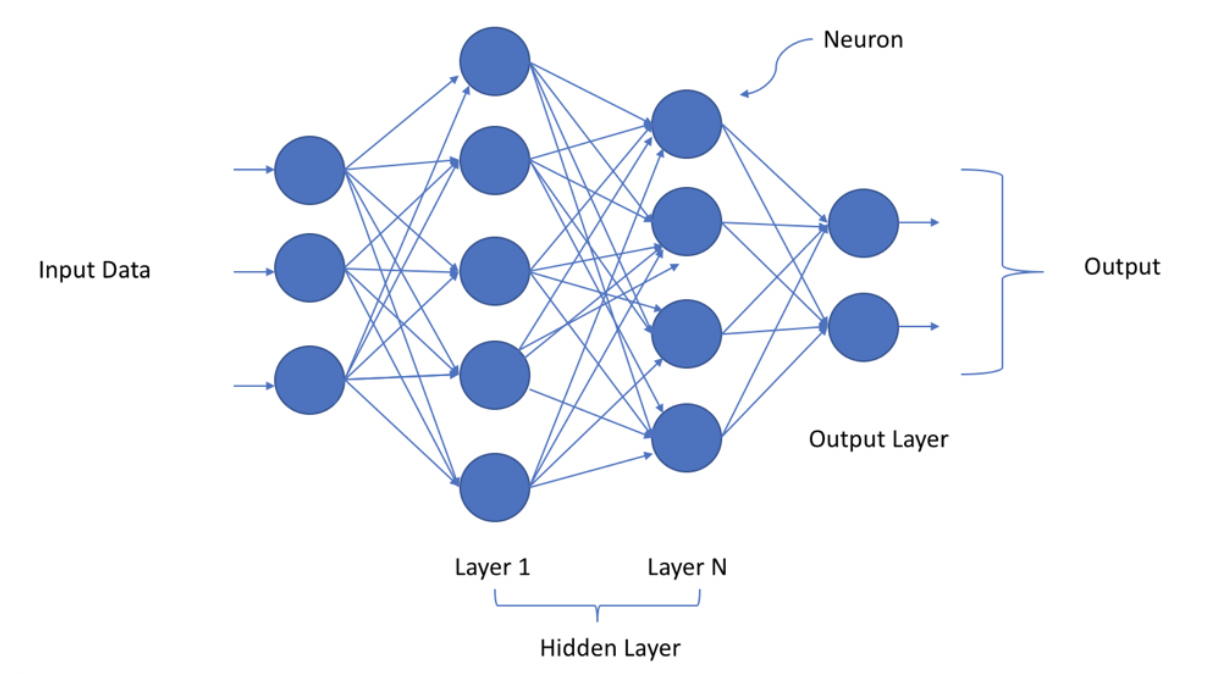
\includegraphics[width=0.95\textwidth]{DNN.png}
            \caption{Deep Neural Network (DNN) basic architecture.}
            \label{fig:dnn}
        \end{figure}
        
Deep neural networks (DNN) are artificial neural networks with multiple hidden layers. A layer is composed of a set of neurons connected to neurons from previous layer. They perform a computation and output a single value sent to the next layer. The neurons together form the neural network. A representation of a deep neural structure can be found \hyperref[fig:dnn]{Figure~\ref*{fig:dnn}}. By combining all the neurons into a coherent ensemble, the neural network should be able to learn complex functions to solve complex problems.

\section{Properties}
Mathematically, for a set of n-1 input values $x_1, x_2, .., x_n$ a neuron will compute the following output:
\[\ out = \sigma( \sum_{i=1}^{n}{x_i \omega+ b })\]
with $\sigma(.)$ a non-linear activation function, $b$ the bias and $w_i$ the weights of the neuron. An illustration of a single neuron is presented in \hyperref[fig:mlp]{Figure~\ref*{fig:mlp}}. To train a neural network, we tune the weights (or parameters) and bias of all neurons in order to produce a specific function.

\begin{figure}[!h]
            \centering
            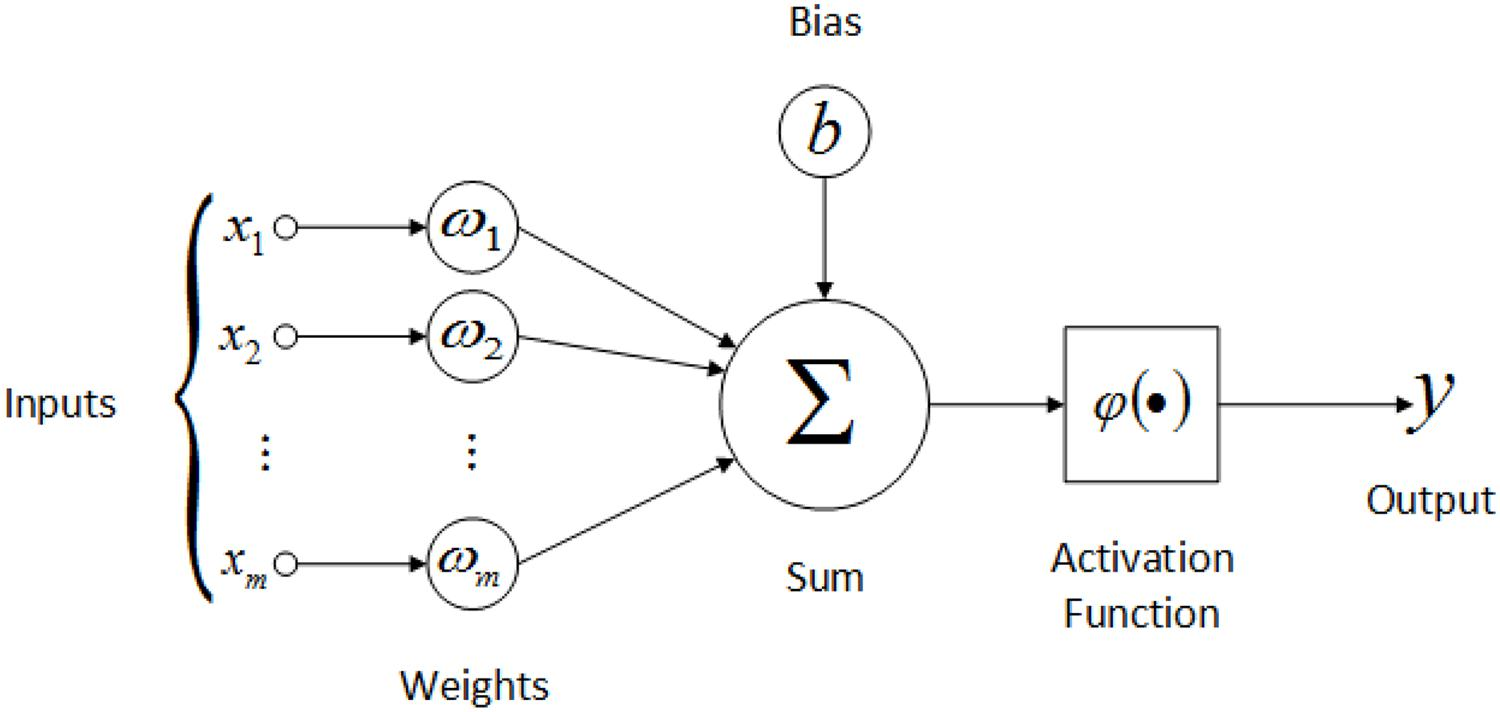
\includegraphics[width=0.45\textwidth]{MLP}
            \caption{Neuron in DNN}
            \label{fig:mlp}
        \end{figure}
  \newline \newline  
The input layer of the neural network get streams of data in different formats like images, audio, or texts. From the dataset, input features with weights and biases are used to calculate the linear function. The result from this function is used by the activation function as input and the output are further used as input to the next layer.
There are several types of activation functions that can be chosen by the context, the most used are the following: Sigmoid function, TanH function, ReLU function \cite{act_function}.
\newline \newline
Basically, three important steps took place in a single iteration of deep neural architectures: Forward Propagation, Backward Propagation, and Gradient Descent(Optimization).
\begin{itemize}
\item \textit{Forward Propagation:} In this phase, input data is sent in the forward way through each layer of the neural network. Here, there is the linear calculation and the application of the activation function.
\item \textit{Back Propagation:} During this step all parameters will be update, calculating their derivates; in this way we obtain a their optimization.
\item \textit{Optimization: }All parameters will be continuously update in order to obtain a convergence of the loss function. Some optimization algorithms are as follows: Gradient Descent, Momentum, Adam, AdaGrad, RMSProp, etc.
\end{itemize}
So we know that  weights and biases are the parameters that should be changed for the network to learn, but it's needed to understand if they should be increased or decreased. An answer to this problem is the implementation of a loss function, that is a mathematical function that link all possible variables into a single value that represents the distance from the optimum (the perfect performance); in other words it shows how much the algorithm is "losing" from optimal state. Where there are poor accuracy, it means that loss function get higher values and it should gradually decrease during learning, reaching zero at the end. The selection of a loss function is one of the most critical decisions that everyone have to do initially.

\chapter{Continual learning}
\label{chap:2}
In the previous chapters, we introduced classical deep learning basic concepts and pipeline and showed their lack of adaptability in practical situations. We also introduced how continual learning aims at solving those shortcomings. In this chapter, we present the continual learning research field more extensively. All theoretical notions and definitions about this framework are introduced in this section. 
\section{Definition of Continual Learning}
Given a potentially infinite amount of data, a Continual Learning method should learn from a sequence of partial experiences where all data is not available at the same time. A non-continual learning setting would then be when the algorithm can have access to all data at once and can process it as desired. CL algorithms can have to deal with imbalanced or scarce data problems \cite{drossos}, catastrophic forgetting \cite{sprechamn} or data distribution shifts \cite{gepperth}.
\newline \newline
Continual Learning is based on the simple, yet fundamental idea of learning continually over time \cite{chen-2018, ring}. The basic intuition is that data are not aprioristically available, like generally assumed in machine learning research, but only in a time-delayed fashion.
\\
This framework, also referred to as Lifelong or Incremental Learning, can be considered as a challenging research problem. 

\section{Brief History and motivation}

The concept of learning continually from experience has always been present in artificial intelligence since its birth \cite{turing,weng}. However, it is only at the end of the 20th century that it has began to be explored more systematically. In the artificial intelligence community, the lifelong learning paradigm has been popularized around 1995 \cite{ring,thrun-mitchell,thrun}. Since then there were four different main area where this topic has been studied:
\begin{itemize}
    \item \textit{Continual Supervised Learning}. Thrun \cite{thrun} was one of the first to study continual learning within a supervised context, where each previous or new task aims at recognizing a particular concept using binary classification.
    \item \textit{Continual Unsupervised Learning}. While intuitively better suited for unsupervised learning, continual learning research in this area have not been extensive and mainly focused on topic modeling and information extraction.
    \item \textit{Continual Semi-Supervised Learning}. The work in this area is well represented by the Never- Ending Language Learner (NELL) system by \cite{carloson}.
    \item \textit{Continual Reinforcement Learning} .First CL algorithms are proposed by Mitchell and Thrun \cite{mithcell-thrun} about robotic learning to capture  the invariant knowledge on each individual task.
\end{itemize}


\newline \newline
While continual learning has been proposed for more than 15 years, researchers and studies in this field has not ever been very considerable. Nevertheless it's becoming a solid interest of the machine learning and AI community only now
Continual Supervised Learning. The reasons for this delay are concentrated in some more complex and fundamental problems that have characterized AI until today.
\begin{itemize}
    \item Lack of systemic approaches: Machine learning research for the past 20 years has focused on statistical and algorithmic approaches on simple tasks (e.g., tasks where the distribution of data is assumed static). Disentangling “static” learning performance from continual learning side effects is important for the very incremental nature of the research and to facilitate comparison between approaches in this area.
    \item Limited amount of data and computational power: Digital data is a luxury of the 21st century. Before the big data revolution, collecting and processing data was a daunting task. Moreover, the limited amount of computational power available at the time did not allow complex and expensive algorithmic solutions to run effectively, especially in a continual learning setting which undoubtedly makes learning more complex by having to deal with multiple tasks at the same time, as well as having to incorporate the concept of time into the learning process.
    \item Focus on supervised learning: creating labelled data is probably the slowest and the most expensive step in most ML systems. This is why learning continuously has been for a long time not a viable and practical option.
    \item Manual engineered features and had-hoc solution: Before early 2000 and early works on representation learning creating a machine learning system would mean to handcraft features and finding had-hoc solution which may differ significantly depending on the task or domain.
\end{itemize}

The achievement of these limits, with all advancements and research in machine learning, as well the fast technological evolution witnessed in the last 15 years, has opened the door for focus on more intricate problems such as learning continually.
In the following chapters we will focus on recent continual learning developments in the context of deep learning, introducing theoretical concept and notions.
\section{State of the art}

The biggest problem faced today by continual learning algorithms is known in literature as \textit{Catastrophic Forgetting} or \textit{Catastrophic Inference} \cite{cat_forgetting}. Neural networks almost often trained with gradient-based optimization methods suffer dramatically from this problem, experiencing a rapid overriding of the model parameters when learning from different data distributions over time. This is reason almost every recent work in the context of deep continual learning has been focusing on such a problem, one of the biggest obstacle to the adoption of AI systems that learn continually.
It's possible contrasting catastrophic forgetting in several ways, and not only through hyper-parametrizations or basic regularization techniques. As we will later discuss in \hyperref[chap:3]{Chapter~\ref*{chap:3}}, many different strategies have been proposed, showing, with different degree of success, that CL can be used in complex domains like computer vision and natural language modeling \cite{parisi}. Early results in this area are promising, even though still to be proven over a long sequence of batches or tasks.

In next section there is a short review of the large number of domains in which continual learning could have an impact is here summarized. All applications that use streams of data in real-time that are not easy to store in fixed data, are the ones which would benefit the most from the integration of CL features. A list of field and applications in which this framework may be beneficial or has been applied can be found below:
\begin{itemize}
    \item Computer Vision: given the high-dimensionality and high-velocity of visual information, computer vision tasks are one of more suitable domains to prove the importance of continual learning and to actually benefit from it also from a practical point of view.
    \item Natural Language Processing & Speech Recognition: Continual learning may substantially improve the human-to-machine interaction through efficient on-device personalization/adaptation. This may not only reduce the computational burden on the server side (and improve the adaptation speed), but given the highly personal nature of the information being processed by the virtual assistants, it may also force the raw data to never leave the device.
    \item Robotics: RL Intelligent Adaptive Curiosity (RL-IAC) is one of the few examples of direct application of CL in a robotic environment for learning visual salience \cite{creaye}. However, the proposed algorithm does not use deep architectures.
    \item Internet of Things: embedded devices with highly constrained hardware resources and operating off-line (due to privacy or operational reasons) may highly benefit the introduction of more efficient learning algorithm operating on real-time data and without the need of storing them. 
    \item Machine Learning Production Systems: machine learning production systems are becoming more and more common in every organization. Being able to fast train and deploy new prediction models over time becomes essential to provide up-to-date and always improving services. 
\end{itemize}
\chapter{Continual learning framework}
\label{chap:3}
We will try to explain continual learning a little more formally in an accurate framework and with additional constraints which allow us to understand better the experiment that will be presented in following sections.
Drawing inspiration from the famous definition of Machine Learning by \cite{michalski}, we could try to summarize continual learning, operatively, in a single sentence as in the following definition.
\newline \newline
A computer program can learn continually from a data stream, giving a sequence of partial experience $E_i$, a target function $h^\ast$ and performance measure P. This performance to optimize $h^\ast$ improves with more processed partial experience $E_i$.
The most important thing is that every single part of data cannot be processed multiple times and if we take them in isolation, they constitute only a partial amount of total data needed to perform the learning.
\newline \newline
In the following sections a comprehensive and complete framework is detailed to help distinguish several approaches in different continual learning settings.
\section{Formal definition}
Early theoretical attempts to formalize the continual learning paradigm can be found in \cite{ring-2005}. 
To give a precise definition of this framework, it is fundamental to clearly describe the data stream, its use, the algorithm functioning, its assumed prior knowledge, and its requirements in terms of supervision, memory and computation.
\newline \newline
\textbf{Definition}: \textit{Continual Learning Algorithm}. In continual learning (CL) data arrives in a streaming fashion as a (possibly infinite) sequence of learning experiences S = $e_1, ..., e_n$. Given X and Y as input and output random variable respectively, let us consider D a potentially infinite sequence of unknown distributions $D={D_1,...,D_n}$ over $X x Y$,we encounter over time(hence with $ n∈[2,...,\infty))$. A continual learning algorithm $A^{CL}$ is an algorithm with the following signature:
\begin{equation}
                \forall D_i\in D, \quad    A^{CL} : \langle h_{i-1}, B_i, M_{i-1}, t_i \rangle \rightarrow  \langle h_i, M_i \rangle. 
\end{equation}

Where:
\begin{itemize}
    \item $h_i$ is the current hypothesis at timestamp i, or, in other words, the parametric model learned continually,i.e.the model learned after training on experience $e_i$.
    \item $M_i$ is an external memory where we can save previous training examples.
    \item $t_i$ is a task label, void if not provided. It can be used to disentangle tasks and specialize the hypothesis parameters, as it is done in \cite{lopez}.
    \item $B_i$ is the training batch of examples. Each $B_i$ is composed of a number of examples $e_i^j$ with $j \in [1,...,m]$. Each example $e_i^j \langle x_i^j, y_j^i \rangle$, where $f^i$ is the feedback signal and can be the optimal hypothesis $h^\ast(x,t)$ (i.e., exact label $y_j^i$ in supervised learning), or any real tensor (from which we can estimate $h^\ast(x,t)$, such as a reward $r_j^i$ in RL).
\end{itemize}
\\
The objective of a CL algorithm is to minimize the loss $L_s$ over the entire stream of data $L_S$:
\begin{equation}
                L_S(h_n,n) = \frac{1}{\sum_{i=1}^{n}{|B_{test}^i|}} * \sum_{i=1}^{n}{L_{exp}(h_n,B_{test}^i)}
\end{equation}

\begin{equation}
                L_{exp}(h_n,B_{test}^i) = \sum_{j=1}^{|B_{test}^i|}{L(h_n(x_j^i),y_j^i)}
\end{equation}

where the loss $L(h_n(x),y)$ is computed on a single sample $\langle x,y \rangle$, such as cross-entropy in classification problems.






\section{Task}
A task is a learning experience characterized by a unique task label t and its target function $g_{\widehat{t}}(x) \equiv h^\ast(x, t = \hat{t})$, i.e., the objective of its learning.
It is fundamental to evidence that the tasks are just an abstract representation of a learning experience represented by a task label. This label is used to divide the complete learning experience into smaller learning parts.
\\
The concept of task is essential in continual learning scenario. Clarify the notion of task from training batch is important in CL since data are not available all at once, but may be as well related to the same learning objective $g_{\widehat{t}}$.
Different scenarios of continual learning framework depends on how the concept of task is treated; more details are introduced in next chapter.

\section{CL Scenarios}
We focus on the continual learning problem in which a single neural network model needs to sequentially learn a series of tasks. During training, only data from the current task is available and the tasks are assumed to be clearly separated. This problem has been actively studied in recent years and many methods for alleviating catastrophic forgetting have been proposed. However, because of differences in the experimental protocols used for their evaluation, comparing methods’ performances can be difficult. In particular, one difference between experimental protocols we found to be very influential for the level of difficulty is whether at test time information about the task identity is available and—if it is not—whether the model is also required to explicitly identify the identity of the task it has to solve.
We can introduce several key-setting that allow to explain different scenarios:
\begin{itemize}
\item \textit{Availability of task/Distribution labels.} The ability of customize specific behavior for objective hypothesis giving label to each task. It makes the continual learning problem much easier
\item \textit{Task/Shift boundaries.} It impacts the complexity of the problem
\item \textit{Experience content}. It stays for the classes that we can find in experience. During batches we can fin the same, new or any classes
\item \textit{Classification problem.} The type of the problem that can be unique or partitioned.
\end{itemize}



\begin{table}[h]
            \centering
            \begin{tabular}{ |c|c|c|c|c|  }
                \hline
                \textbf{Name} & \textbf{Task Labels} & \textbf{Boundaries} & \textbf{Classes} & \textbf{Problem}\\
                \hline \hline
                Class-Incremental & no & yes &  new & unique\\
                \hline
                Task-Incremental & yes & yes &  new & partitioned\\
                \hline
                Domain-Incremental & no & yes &  same & unique\\
                \hline
                Task-Free & no & no &  any & unique\\
                \hline
                Task-Agnostic & no & no &  any & partitioned\\
                
                
                \hline 
                
            \end{tabular}
            
            \caption{Key-Setting and Scenarios}
            \label{tab:vggrob}
        \end{table}

The most three relevant continual learning scenarios are the following: Task-Incremental, Class-Incremental, Domain-Incremental.
\begin{table}[h]
            \centering
            \begin{tabular}{ c|c  }
                \hline
                \textbf{Scenario} & \textbf{Required at test time}\\
                \hline \hline
                Task-Incremental & Solve tasks so far, task-ID provided\\
                \hline
                Class-Incremental & Solve tasks so far, task-ID provided\\
                \hline 
                Domain-Incremental & Solve tasks so far, task-ID not provided\\
               
                
                
                \hline 
                
            \end{tabular}
            
            \caption{Key-Setting and Scenarios}
            \label{tab:vggrob}
        \end{table}
In the first scenario, models are always informed about which task needs to be performed. Task-incremental learning (Task-IL) is the easiest continual learning scenario where task identity is always provided and it is possible to train models with task-specific components. A typical network architecture used in this scenario has a “multi-headed” output layer, meaning that each task has its own output units but the rest of the network is (potentially) shared between tasks.
\\
In the second scenario, called domain-incremental learning (Domain-IL), task identity is not available at test time. Models have to solve the task at hand; they are not required to infer which task it is. There are some examples of this scenario, like protocols where the structure of the tasks is always the same, but the distribution of the input is changing. A relevant real-world example is an agent who needs to learn to survive in different environments, without the need to explicitly identify the environment it is confronted with.
\\
Finally, in the third scenario, models must be able to both solve each task seen so far and infer which task they are presented with. It's named class-incremental learning (Class-IL) because it includes the common real-world problem of incrementally learning new classes of objects.
\subsection{CL Scenarios categorization}
Nowadays it's quite difficult provide a comprehensive and general categorization that that would be reasonable across all continual learning fields. One possible categorization is based by how the task of the stream data is treated.
A CL scenario is a specific CL setting in which the sequence of N task labels respects a certain “task structure” over time. Depending on the task-awareness or task-agnosticism of the problem to learn, now we can define, on a more abstract level and based on the specific $t$ signal availability, three different and common scenarios for CL based on the proposed framework:
\begin{itemize}
\item \textit{Single-Incremental-Task (SIT): }$t_1 = t_2 = ... = t_N$
\item \textit{Multi-Task: }$ \forall i,j \in [1, .., n], t_i \neq t_j $
\item \textit{Multi-Incremental-Task:} $\exists i,j,k: t_i = t_j$ and $t_j \neq t_k$
\end{itemize}
In the following sections we discuss each scenario more in detail.
 \subsubsection{Single-Incremental-Task}
 The Single-Incremental-Task (SIT) is a very general scenario where we don’t have a different task supervised signal for every training batch. It can be considered as solving a single task, which is incremental in nature or just to be in a “task agnostic” setting where data can be treated to similar or very different data distributions over time. However, it may be useful, also in this case, to detect and recognize very different data distributions to specialize the behavior of the agent even without the external supervised notion of task.
 
 
  \subsubsection{Multi-Task}
  The Multi-Task (MT) scenario constitutes a typical setting for recent literature in CL where it is assumed to encounter a number of subsequent tasks over time, each corresponding to a different training batch with very different data distributions \cite{parisi}. While this setting is useful for assessing continual learning strategy, it may revel itself less appropriate for modeling real-word problems where we can encounter many different batches of data over time, related to the same task or encounter the same task many times over our lifetime.
  
   \subsubsection{Multi-Incremental-Task}
   The Multiple-Incremental-Task (MIT) scenario constitutes the more realistic scenario in which we consider natural to be able to exploit some supervision (like parents teaching in humans) or feedbacks about the tasks we are tackling over time. This allows the agent to learn task-related specialized behaviors as well the autonomous development of its generalization capabilities.
\subsection{Update Content Types}
\label{chap-332}
This concept has the same importance of the previous categorization; they are two arguments strictly correlated.
We can consider three different Update Content Type (UCT) which may greatly impact on the complexity of the continual learning scenario. They refer to the possible kind of data contained in each training batch $B_i$:
\begin{itemize}
    \item \textit{New Instances (NI):} in this case the content of the batch is characterized by new instances (i.e. examples) of the same classes encountered in the previous batches.
    \item \textit{New Classes (NC):} the content of every batch $B_i$ is based on the presence of examples belonging to different classes never encountered in previously batches $B_1,...,B_{i−1}.$
    \item \textit{New Instances and Classes (NIC):} this update content type constitutes the the most realistic setting where new examples of previous encountered classes but also new classes are encountered over time.
\end{itemize}

In order to semplify the concept of Content Update Type, let us recover the aforementioned example of classification. If an algorithm learns the cat vs dogs classification problem on a dataset and then new images of cat vs dogs are provided to the algorithm, we are then in a New Instances case (NI), we have new data but no new concepts. If the new instances were of different classes (e.g. cars vs bikes) we then would face the New Concepts case (NC). The new instances and new concepts case would then have been a mix of both new images of known and new classes.
\section{CL strategies}
\label{chap-3-4}
Nowadays there is no exist formal categorization about continual learning methodologies.
While the community has not agreed yet on a shared categorization for CL strategies, we present a summary of the most popular continual learning strategies in four literature based on \cite{kemker,zenke}. There is no formal definition for each of those categories so this makes very difficult to understand if a particular algorithm or strategy belongs to one category or another so it really depends on a specific view of a researcher. It's reasonable to assume for example a a four way fuzzy categorisation:
\begin{itemize}
    \item Regularization Strategies
    \item Generative Replay Strategies
    \item Rehearsal Strategies
    \item Architectural Strategies
\end{itemize}
\begin{figure}[!h]
            \centering
            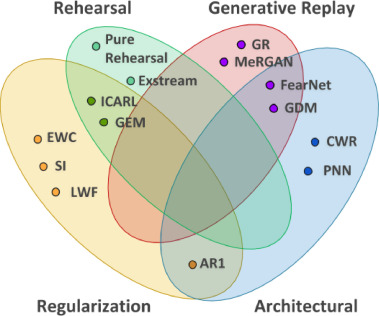
\includegraphics[width=0.65\textwidth]{cl_strategies.jpg}
            \caption{Figure from \cite{lomonaco}. Continual learning strategies categorization.}
            \label{fig:cl_strategies}
        \end{figure}

Assuming that Rehearsal strategies can be considered also as a type of Replay strategies, we can also introduce another 3-way categorization. In the following figure different strategies are introduced under their general group. More details about them are written in next sections.

\begin{figure}[!h]
            \centering
            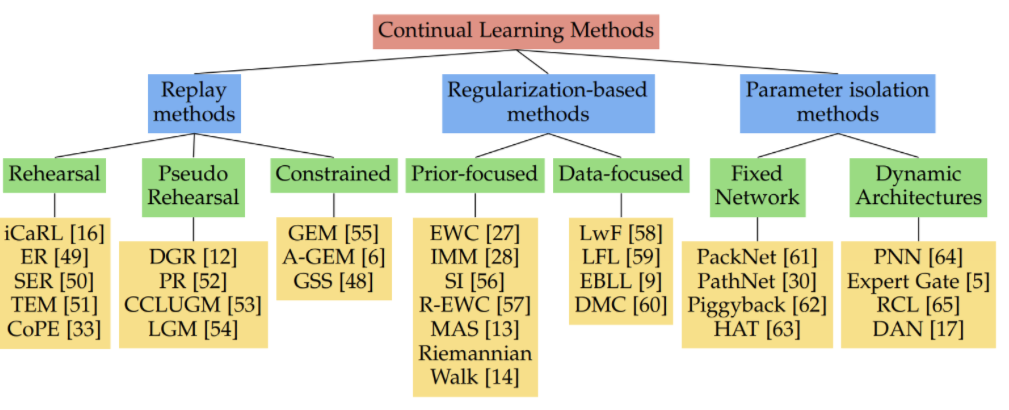
\includegraphics[width=0.8\textwidth]{cl_3strategies.png}
            \caption{Continual learning strategies 3-way categorization.}
            \label{fig:cl_strategies}
        \end{figure}
        
        
\subsection{Baseline Strategies}
Before moving to more elaborated continual learning strategies, let us consider four basic approaches:
\subsubsection{Naive} The Naive strategy simply finetunes the model across the training batches without any specific mechanism to control forgetting, except early stopping and other basic regularization techniques like L1, L2 and Dropout \cite{goodfellow-2013}, which have been already found to avoid overfitting and improve generalization. In other words it is just continue fine tuning back propagation optimization step on the new observations and new examples.
\subsubsection{JointTraining - Offline} We have a second common baseline that is a joint training or often called offline strategy. Assuming that you have access to all the data related to all the experiences at the same time, it can be considered as a pure multi-task learning
\subsubsection{Ensemble} Basically we have a separate model for each experience and we use them together doing inference for testing.
\subsubsection{Cumulative} The Cumulative strategy, also called Full Rehearsal \cite{hayes}, limits catastrophic forgetting by mixing all older examples with the new examples to be learned. When a new batch of data becomes available, there are two viable options: 
\begin{itemize}
    \item Finetuning $h_{i - 1}$ with all the cumulated patterns
    \item Start from scratch (i.e. from random weights initialization)
\end{itemize}
The cumulative learning strategy is indeed very similar to the classical multi-task training setting \cite{caruana}, which is known to yield even better performance than learning every single task in isolation.
\subsection{Rehearsal Strategies}
Rehearsal strategies are based on the idea of rehearsing past knowledge with a replay mechanism. Most of these strategies employ a fixed-sized external memory in which to store representative examples to reuse in conjunction with the new coming data in order to improve generalization without forgetting; in this way we can reuse for rehears activities that consists  in mixing those patterns with the new acquired observations and research the knowledge we have previously applied. In other words past information is periodically replayed to the model to strengthen connections for memories it has already learned. It can be defined as a simple approach that stores part of the previous training data and interleaves them with new patterns for future training. 
\\
An example of strategy in this class is Exemplar Stream (\textit{ExStream}) that was firstly introduced by \cite{hayes} as a partitioning- based method for stream clustering and the efficient management of the external fixed-size memory for rehearsal. Its performance depends on the external memory size and the task at hand.
\subsection{Generative Replay Strategies}
In this set of strategies the idea is that we do not preserve specific set of examples exactly as they are seen in the past but this approach train generative models on the data distribution. Therefore, they are able to afterwards sample data from past experience when learning on new data. By learning on actual data and artificially generated past data, they ensure that the knowledge and skills from the past is not forgotten. These methods have also been associated with the term pseudo-rehearsal \cite{robins} . A typical way to implement a generative replay is through dual models. The first one (called 'frozen') that generates samples from previous experiences and the second one learns to produce and classify current patterns with to the regenerated ones previously.  When a task is over, we replace the frozen model by the current one, freeze it, and initialize a new model to learn next task. After this definition of Generative Replay strategies, many research group this set and the previous one under the same group because both use a replay mechanism. Most of the Generative Replay based approaches are meant to solve classification tasks but there are other ones that are used for unsupervised learning or reinforcement learning.

\subsection{Architectural Strategies}
Architectural Strategies are based on the central idea of modifying the model architecture and parameters value in order to preserve old information and make space to the incoming one. Modifying connections, activation functions, freezing parameters to mitigate forgetting are very common possibilities. These strategies can be defined also dynamic because these changes to make to the architecture of a model must be done dynamically, in order to earn new concepts or skills without interfering with old ones. One of the most relevant strategy in this group is \textit{PNNs} (Progressive Neural Network). 
\\
They were originally proposed by \cite{rusu} for explicitly tackling catastrophic forgetting and are one of the best examples of the architectural category. The idea is to keep a pool of pre-trained models (or “columns”) as knowledge base, and use lateral connections between them for fast adaptation to the new batch/task.


\subsection{Regularization Strategies}
This set of strategies is based on the concept of Regularization; it is a process of introducing additional information in order to prevent overfitting. In the context of Continual Learning, the central idea is based on regularizing the learning process on the new data for preserving past learned knowledge and skills; the model should not overfit a new problem because it would make it forget it’s previous skills. These approaches consist in changing the update of weights during learning in order to keep memory of previous knowledge.
The regularization methods are more efficient in reinforcement learning \cite{Kirkpatrick}, classification \cite{chelsea} and also generative models. A limitation is that after several tasks the model may saturate because of a too high regularization, and finding a good trade-off between regularization that allows learning without forgetting may be hard.
\newline \newline
In the following sections, most important strategies of this set are explained.

\subsubsection{Elastic Weight Consolidation (EWC)}
The Elastic Weight Consolidation (EWC) methodology helps to reduce catastrophic forgetting by regularizing parameters of a network trained on previous tasks by penalizing any their change according to their relevance. It can be defined also as a regularization approach which  control forgetting by selectively constraining (i.e., freezing to some extent) the model weights which are important for the previous tasks \cite{ewc}. Once a model has been trained on a task, thus reaching a minimum in the loss function, the sensitivity of the model w.r.t. each of its weight $\theta_k$ can be estimated by looking at the curvature of the loss surface along the direction determined by $\theta_k$ changes. So, we can say that an high curvature means that a little $\theta_k$ change brings in a effective increase of the loss. A main role in this strategy is assumed by Fisher information matrix FIM \cite{fisher}. The diagonal of the Fisher information matrix F, which can be computed from first-order derivatives alone, is equivalent to the second derivative (i.e. curvature) of the loss near a minimum. Therefore, the $k^{th}$ diagonal element in F (hereafter denoted as $F_k$) denotes the importance of weight $\theta_k$. Important weights must be moved as little as possible when the model is fine-tuned on new tasks.
\newline \newline
If we consider a sequence of tasks or batches $B_i$ and after training the model on batch $B_i$, it's necessary to calculate the Fisher information matrix $F_i$ and save the set of optimal weights $\Theta^i$. $F_i$ and $\Theta^i$ will be then used to regularize the training on $B_{i+1}$. Each diagonal element $F_k^i$ can be computed as the variance of $\varphi L_{cross}(\hat{y},t)/\varphi \Theta_k$ over the $n_i$ patterns of $B_i$.

To sum up, EWC is reasonably simple and, for every batch $B_i$, its overhead consists of:
\begin{itemize}
    \item calculation of Fisher information $F^i$, requiring one forward and one backward propagation for each of the $n_i$ samples.
    \item storage of F and $\Theta$, totaling $2m$ values (m is the amount of model weights).
   
\end{itemize}
\begin{figure}[h]
            \centering
            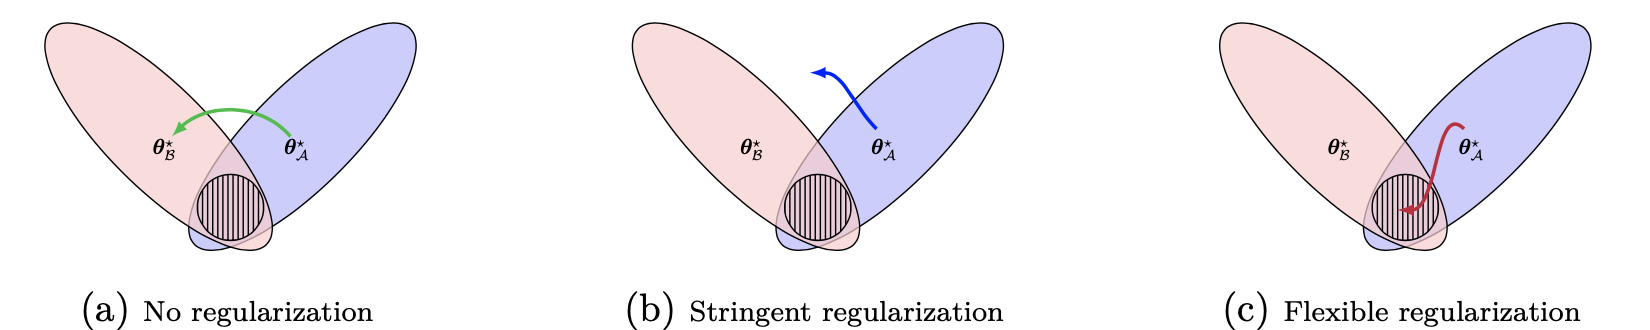
\includegraphics[width=0.95\textwidth]{ewc.png}
            \caption{Sequential training on task B after task A. (a): Train the network as it is: results in ‘Forgetting’, (b): Make no change in the parameters of previous tasks, (c): Make changes in the parameters of the previous tasks depending on their importance.}
            \label{fig:ewc}
        \end{figure}
In the following \hyperref[fig:ewc]{Figure~\ref*{fig:ewc}}  more cases of different regularization are presented. First figure (fig a) represents the case when we simply fine-tune the network on the subsequent tasks. By this way, the network learns the optimum parameters according to the current task, resulting in forgetting. Figure b shows the case when there is a strict regularization to the parameters learnt from the previous tasks. This method doesn’t compute the relevance of the parameters and penalizes all of them in the same way. Consequently network forgets the previous task and it isn't able to learn the current one. Finally, fig c refers to the EWC methodology of computing the importance of parameters before fine-tuning on next tasks. This ensures that the network learns the optimum parameters that performs well for all tasks.
\subsubsection{Learning without Forgetting (LWF)}
Learning Without Forgetting (LWF) [Li and Hoiem, 2016] is a regularization approach which tries to control forgetting by imposing output (i.e. prediction) stability via distillation. It has been originally conceived for a Multi-Task (MT) setting but it can be also easily adapted to other scenario.
\\
Distillation techniques were introduced by \cite{distillation} in order to transfer knowledge from neural network A to neural network B. The idea is that after A has learned to solve a task, we want B to share this skill with A. We then forward the same input to both A and B and impose B to have the same output as A. This technique should be more successful than retraining B because A produces a different target that helps B to learn faster. In order to apply this method for continual learning, after network A learned to solve the first task, and while B is learning the second one, we distill knowledge from A to B. In the end, B should be able to solve both tasks. A drawback of distillation is that it generally needs to preserve a reservoir of persistent data learned for each task in order to apply distillation from a teacher model to a student model
\subsubsection{Synaptic Intelligence (SI)}
Synaptic Intelligence (SI) was introduced in \cite{zenke} as a variant of EWC. The computation of Fisher information matrix during EWC is expensive for continual learning and it was proposed to determine weight relevance in SGD process.
SI setting is moderately comprehensible and, for every batch $B_i$, its overhead consists of:
\begin{itemize}
    \item computation of weight relevance $F^i$, based on information previously accessible during SGD.
    \item storage of F and $\Theta$ consist in $2m$ values (m is the amount of model weights).
\end{itemize}



\part{Continual Learning for Event Audio Classification}
\chapter{Avalanche}
\label{chap5}
\section{Overview}
Avalanche \cite{avalanche} is an open-source end-to-end library supported by the non-profit organization \textit{ContinualAI} for Continual Learning research \& development based on the popular ML frame- work \textit{PyTorch} \cite{pytorch}. Avalanche is designed to provide a shared and collaborative codebase for fast prototyping, training, and reproducible evaluation of CL algorithms. We report the operational representation of the framework as presented in its paper in the following \hyperref[fig:avalanche]{Figure~\ref*{fig:avalanche}} .

\section{Components}
\label{avalanche_compoments}
Avalanche is organized into five main modules: Benchmarks, Training, Evaluation, Models, and Logging. We will give an overview of the purpose of each as the work of this thesis is concerned with the whole structure, but we refer to \cite{avalanche} for additional insights on the motivations for such decomposition.

\begin{figure}[h]
            \centering
            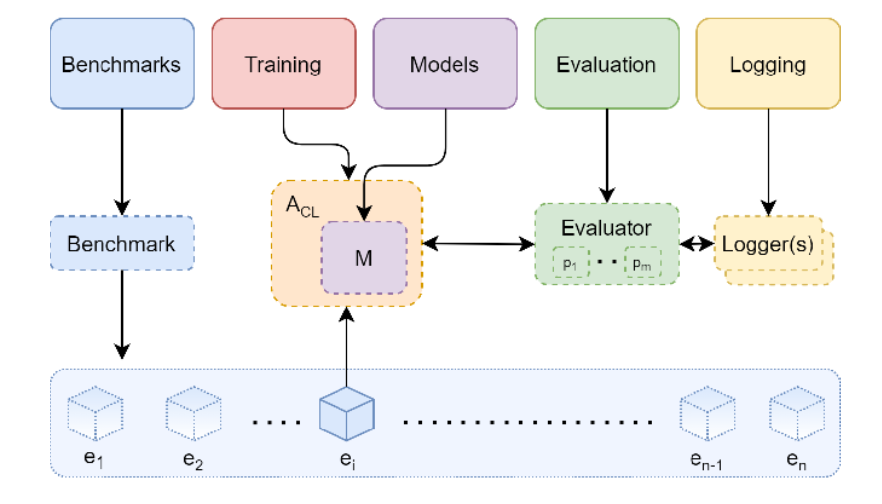
\includegraphics[width=0.75\textwidth]{avalanche.png}
            \caption{Figure from \cite{avalanche}. Operational representation of Avalanche with its main modules (top), the main object instances (middle) and the generated stream of data (bottom). A Benchmark generates a stream of experiences $e_i$ which are sequentially accessible by the continual learning algorithm $A^{CL}$ with its internal model M. The Evaluator object directly interacting with the algorithm provides a unified interface to control and compute several performance metrics ($p_ii$), delegating results logging to the Logger(s) objects.}
            \label{fig:avalanche}
        \end{figure}
        
\subsubsection{Benchmarks}
This module maintains a uniform API for data handling: mostly generating a stream of data from one or more datasets; this is the core abstraction over the task stream formalism which is distinctive of CL. It also contains all the major CL benchmarks (similar to what has been done for \textit{torchvision}). A benchmark can be defined as combination of a scenario with one or multiple datasets that we can use to asses our continual learning algorithms. This module offers 3 types of utils:
\begin{itemize}
    \item \textit{Dataset:} all the Pytorch datasets plus additional ones prepared by our community and particularly interesting for continual learning.
    \item \textit{Classic Benchmarks:} typical benchmarks used in CL literature ready to be used with great flexibility.
    \item\textit{ Benchmarks Generators:} a set of functions that allow to create your own benchmark starting from any kind of data and scenario. There are two type of generators:
    \begin{itemize}
        \item Specific: benchmark are based on a clear scenarios and Pytorch dataset(s). Scenario can be based on NC (New Class) or NI (New Instance) as explained in \hyperref[chap-332]{Section~\ref*{chap-332}} 
        \item Generic: new benchmark are more generic, flexible and customizablle.
    \end{itemize}

\end{itemize}

\subsubsection{Training}
\textit{}This component provides all the needed tools concerning model training. It includes clear and efficient ways of implementing new algorithm as well as a set pre-implemented CL baselines and state of the art strategies. Each of them in Avalanche has two different methods: one for training (train) and another one for evaluation (eval), which can work either on single experiences or on whole stream of data. Currently, Avalanche library provides 11 continual learning algorithms (\hyperref[tab:avalanche_featurs]{Figure~\ref*{tab:avalanche_featurs}}), that can be used to train baselines in a simple way, as shown in \hyperref[fig:avalanche_setup]{Figure~\ref*{fig:avalanche_setup}}. This module includes two main components:
\begin{itemize}
    \item \textit{Strategies}: these are popular baselines already implemented for you which you can use for comparisons or as base classes to define a custom strategy.
    \item \textit{Plugins}: these are classes that allow to add some specific behaviour to your own strategy. The plugin system allows to define reusable components which can be easily combined together (e.g. a replay strategy, a regularization strategy). They are also used to automatically manage logging and evaluation.
\end{itemize}

\subsubsection{Evaluation}
It is a component that provides all the utilities and metrics that can help evaluate a CL algorithm. Its performance should be assessed by monitoring multiple aspects of the computation. This is mostly done through the Metrics: a set of classes which implement the main continual learning metrics computation. Metrics module do not specify in which format their output should be displayed, while loggers do not alter metrics logic. An additional object provided by this module is the Evaluation Plugin: it is the component responsible for the orchestration of both plugin metrics and loggers.
In Avalanche, we can find pluggable metrics monitors such as (Train/Test/Batch) Accuracy, RAM, CPU and GPU usage. A full available list of metrics are reported in \hyperref[tab:avalanche_featurs]{Figure~\ref*{tab:avalanche_featurs}}. 


\subsubsection{Models}
This component contains several model architectures and pre-trained models that can be used for continual learning experiments (similar to\textit{ torchvision.models}). It offers a set of simple neural network architectures ready to be used in experiments. This module allow to focus the attention on Avalanche features and to avoid to concentrate on detail deep architectures.

\subsubsection{Logging}
\textit{}It includes advanced logging and plotting features, including native \textit{stdout}, file and \textit{TensorBoard} support. Avalanche at the moment supports four main Loggers:
\begin{itemize}
    \item \textit{InteractiveLogger}: This logger provides a nice progress bar and displays real-time metrics results in an interactive way (meant for stdout).
    \item \textit{TextLogger}: This logger, mostly intended for file logging, is the plain text version of the InteractiveLogger. Keep in mind that it may be very verbose.
    \item \textit{TensorboardLogger}: It logs all the metrics on Tensorboard in real-time. Perfect for real-time plotting.
    \item \textit{WandBLogger}: It leverages Weights and Biases tools to log metrics and results on a dashboard. It requires a\textit{ W&B} account.
\end{itemize}

\begin{table}[h!]
            \centering
            \begin{tabular}{ |c|p{86mm}|  }
                \hline
                \textbf{Components} & \textbf{Supported features}\\
                \hline \hline
                Benchmarks & \textit{Split/Permuted/Rotated MNIST, Split Fashion Mnist, Split Cifar10/100/110, Split CUB200, Split ImageNet, Split TinyImageNet, Split/Permuted/Rotated Omniglot, CORe50, OpenLORIS, Stream51}.\\
                \hline
                Scenarios & \textit{Multi Task, Single Incremental Task, Multi Incremental Task, Class incremental, Domain Incremental, Task Incremental, Task-agnostic, Online, New Instances, New Classes, New Instances and Classes.}\\
                \hline
                Strategies & \textit{Naive (Finetuning), CWR, Replay, GDumb, Cumulative, LwF, GEM, A-GEM, EWC, Synaptic Intelligence, AR1, Joint Training.}\\
                \hline
                Loss (user specified), Metrics & \textit{Accuracy, CPU Usage,Multiply, GPU usage, RAM usage, Disk Usage, Timing,Confusion Matrix, Forgetting and Accumulate.}\\
                \hline
                Tensorboard Logger, Loggers & \textit{Text Logger, Interactive Logger Weights and Biases Logger (in progress)}.\\

                \hline 
            \end{tabular}
            
            \caption{Avalanche supported features}
            \label{tab:avalanche_featurs}
        \end{table}

 
In addition, the core concepts you will find embedded in Avalanche design are Strategies: they are intended as an abstraction over a particular learning algorithm, which consume experiences from the stream defined by a benchmark and implement the training and evaluation loop. Both loops are composed of a series of well-defined steps which in turn expose a rich callback system: each step is in fact preceded and followed by a callback of the form before step and after step. All strategies inherit and extend Base Strategy, which by default iterates the experience stream, runs a configurable number of epochs on the dataset contained on each and optimizes a given loss function. Note that in the default behavior no Continual Learning technique takes place. To “inject” CL methods Avalanche makes use of Plugins: they operate latching on the call- back system defined by Strategies and are designed in such a modular way so that they can be easily composed to provide hybrid behaviors. Furthermore, comparison with baselines should be a matter of simply removing plugins.
Examples of Strategies include the Naive one, which is so called because it does not add any behavior to the default Base Strategy, thus incurring in catastrophic forgetting; it is commonly used to provide experiments “lower-bounds”. The Replay Strategy instead augments the standard capabilities by making use of configurable memory, which is used to store samples of past experiences to be leveraged during training. 

        
        
\section{Example: Avalanche setup}

\begin{figure}[h]
            \centering
            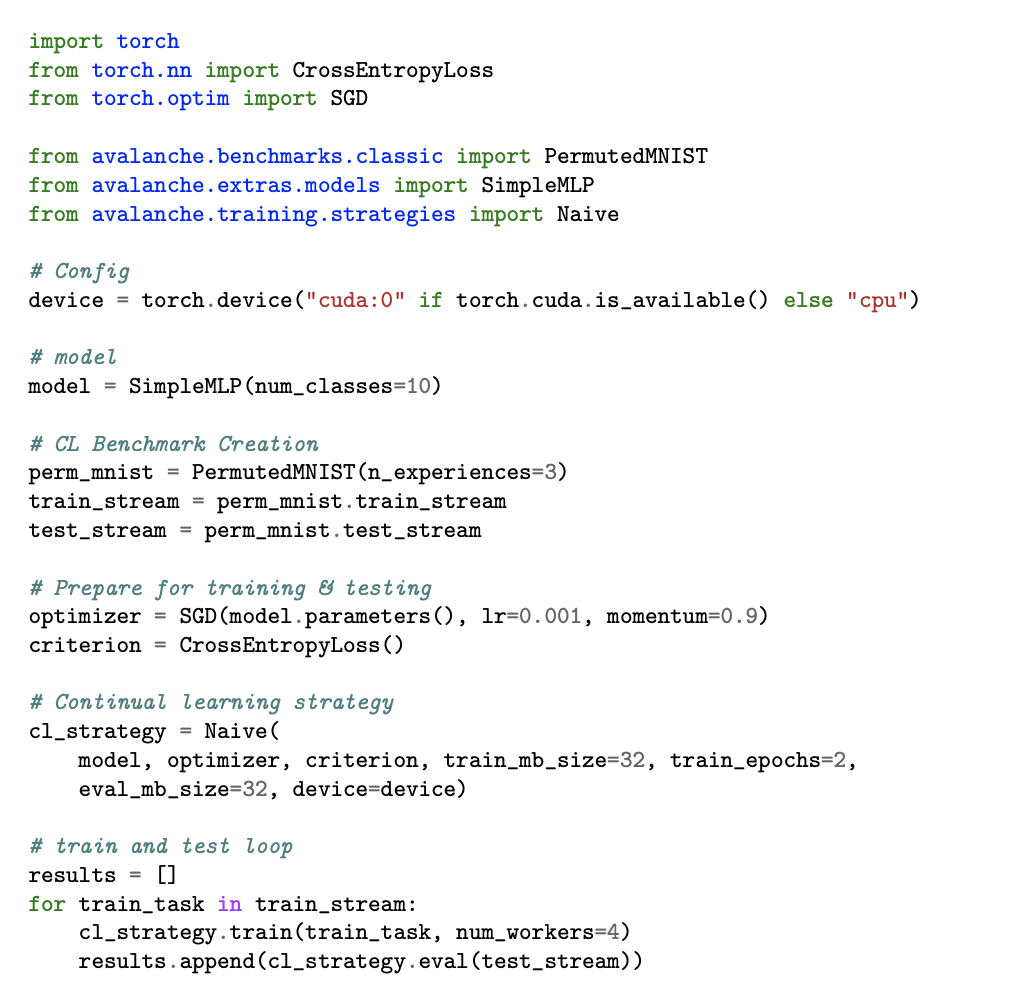
\includegraphics[width=0.70\textwidth]{example_avalanche.png}
            \caption{Example of a typical Avalanche setup.}
            \label{fig:avalanche_setup}
\end{figure}
\hyperref[fig:avalanche_setup]{Figure~\ref*{fig:avalanche_setup}} represents a simple way to implement a continual learning strategy and how use it on a pre-defined benchmark. We start by instantiating a Pytorch model (SimpleMLP) and creating  the continual learning scenario. In this case it's created \textit{PermutedMNIST}, stream of three experiences based on \textit{MNIST} dataset provided by the library from Pytorch dataset. We also define the optimization technique and loss function that are the base of out training and evaluate process. Finally we create the CL strategy: Naive strategy giving in input some object, such as defined model, created benchmark, optimization methods, loss function type and other features (mini batch size and epochs). After strategy definition we proceed with training and evaluation phases. By default, accuracy and loss metrics are included but it's possible to add some metrics with different loggers. 

\chapter{The basic problem: Environmental Audio Classification}
\label{audio}
The main topics of machine listening research have been speech and music. Even though these are just two of the many sound sources that can be heard in most environments, the analysis of environmental sounds has been limited until recently. The lack of, first, public annotated data and, second, a common vocabulary for it have been causes for the scarce research in this field.
In this field a brief overview on audio classification is addressed, introducing a typical Audio dataset that will be used for the experiments in Continual Learning context. 

\section{Audio classification: Overview}
Audio classification or sound classification can be referred as the process of analyzing audio recordings. This amazing technique has multiple applications in the field of AI and data science such as chatbots, automated voice translators, virtual assistants, music genre identification, and text to speech applications.
Below are four types of classification and related use-cases for each.
\begin{itemize}
    \item \textit{Acoustic data classification:} also known as acoustic event detection, it identifies the location where an audio was recorded. This means differentiating between environments such as schools, restaurants , homes, streets, etc. A typical use of acoustic event detection is the building and maintaining of sound libraries for audio multimedia. It also has a role in ecosystem monitoring.
    \item \textit{Environmental sound classification}: just suggested by the name, this is the classification of sound that are in different environments. Recognizing urban sound samples such as car horns, roadwork, sirens, etc.. , can be considered as a valid example of this scenario.  It is also used for predictive maintenance by detecting sound discrepancies in factory machinery. 
    \item\textit{ Music classification:} it is the classification process of the music based on aspects like genre or instruments played. This technique plays a key role in organizing audio libraries by genre, improving recommendation algorithms, and discovering trends and listener preferences through data analysis.
    \item\textit{ Natural language utterance classification}: This is the classification of natural language recordings based on language spoken, semantics, dialect, or other language aspects. In other words, the classification of human speech. This type of audio classification is most common in virtual assistants, but it is also dominant in text to speech applications.
\end{itemize}

In this thesis we focus on Environmental sound classification and we use \textit{ESC-50 dataset }\cite{esc} for experiments that will be presented in next chapters.

\section{ESC Dataset}
This ESC (\textit{Environmental sound classification}) dataset is one on the most useful set of data about audio classification scenario. It consists of three different parts: 
\begin{itemize}
    \item\textit{ ESC-50: }the main labeled set comprising 50 classes of various environmental sounds;
\textit{}    \item \textit{ESC-10:} a small proof-of-concept subset of 10 classes selected from the main dataset - serving as a simplified benchmark.
    \item \textit{ESC-US:} a supplementary dataset of unlabeled excerpts suitable for unsupervised learning experiments.
\end{itemize}
\\
The most suitable and eligible dataset to experiment continual learning strategy about audio classification field, is the ESC-50 Dataset.

\subsection{ESC-50}
The ESC-50 dataset consists of 2 000 labeled environmental recordings equally balanced between 50 classes (40 sounds per class). They are divided in 5 main categories (10 classes per category):
\begin{itemize}
    \item animal sounds;
    \item natural soundscapes and water sounds;
    \item human (non-speech) sounds;
    \item interior/domestic sounds;
    \item exterior/urban noises,
\end{itemize}
The goal of the extraction process was to keep sound events exposed in the foreground with limited background noise when possible. However, field recordings are far from sterile, thus some clips may still exhibit auditory overlap in the background.
The dataset provides an exposure to a variety of sound sources - some very common (laughter, cat meowing, dog barking), some quite distinct (glass breaking, brushing teeth) and then some where the differences are more nuanced (helicopter and airplane noise).
One of the possible deficiencies of this dataset is the limited number of clips available per class. This is related to the high cost of manual annotation and extraction, and the decision to maintain strict balance between classes despite limited availability of recordings for more exotic types of sound events. Nevertheless, it will, hopefully, be useful in its current form and is a concept that could be expanded on if sufficient interest is expressed.
\newline \newline
All 50 classes are presented in the following \hyperref[fig:escclasses]{Figure~\ref*{fig:escclasses}}, with each own major category.
\begin{figure}[h]
            \centering
            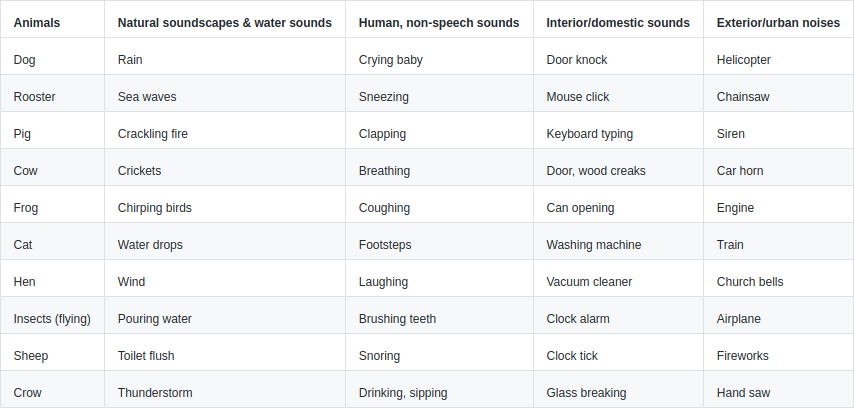
\includegraphics[width=0.90\textwidth]{esc50.png}
            \caption{List of classes in ESC-50 dataset.}
            \label{fig:escclasses}
\end{figure}

\section{How perform audio classification:}
\label{5-3}
Referring to the thesis work, we remind you that this introduction on audio classification was made since the aim of this work is to test Continual Learning strategies on audio-type data, referring to the Environmental Sound Classification scene.
All step and processed work  have been made through language Python with several libraries that allow to download and manage audio data type, as we can see in the following steps represented in \hyperref[fig:audio_step]{Figure~\ref*{fig:audio_step}}.

\begin{figure}[h]
            \centering
            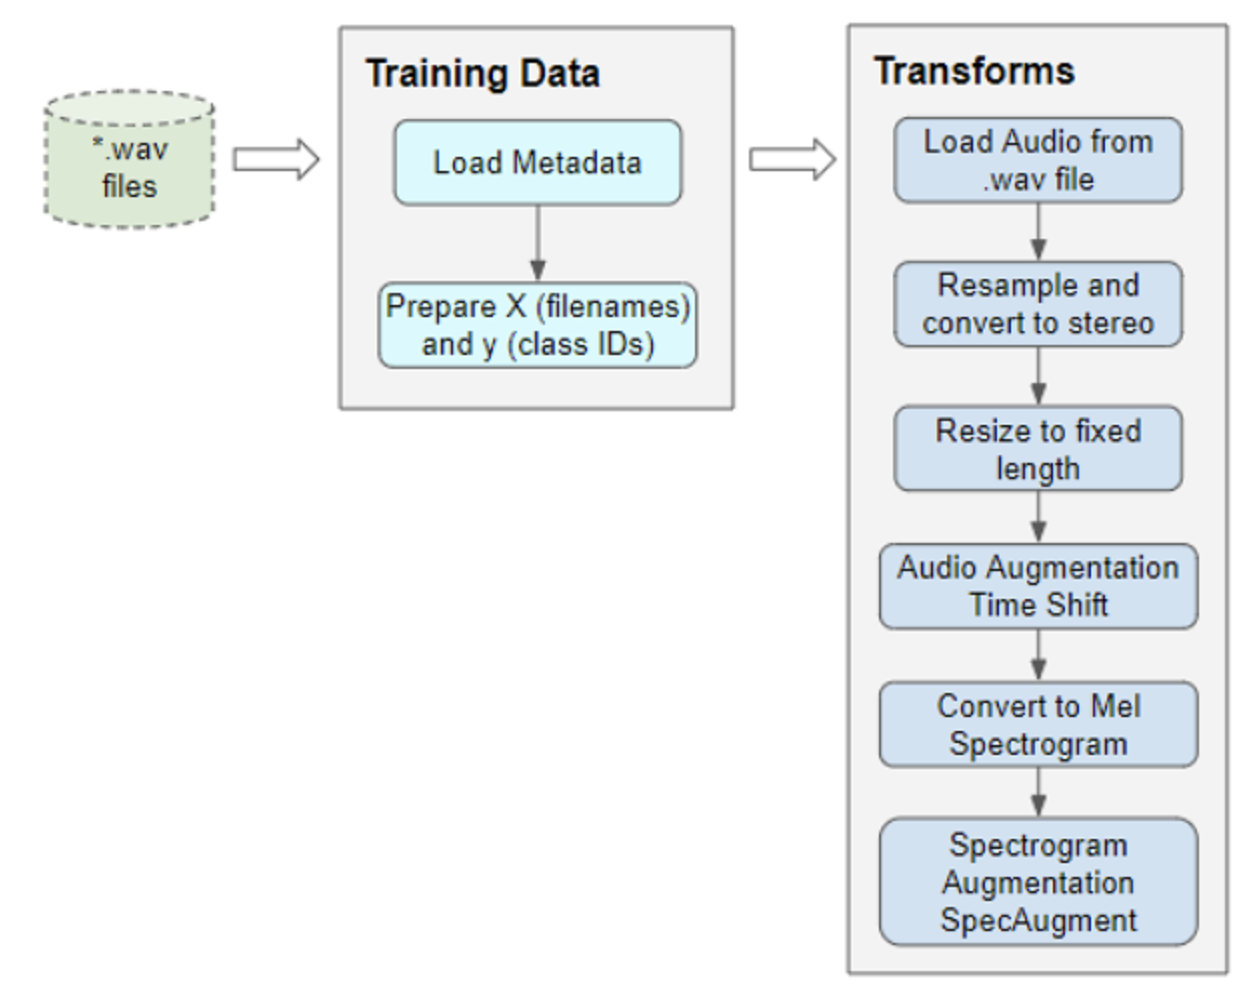
\includegraphics[width=0.70\textwidth]{audio_step.png}
            \caption{Steps for audio classification.}
            \label{fig:audio_step}
\end{figure}


\subsubsection{Read audio from a file}
The first thing we need is to read and load the audio file in “.wav” format (\hyperref[fig:wave]{Figure~\ref*{fig:wave}}). Since we are using Pytorch \cite{pytorch} for this experiment, the implementation uses \textit{Torchaudio} \cite{torchaudio} and \textit{Librosa} \cite{librosa} for the audio processing.


\subsubsection{Standardize sampling rate}
Some of the sound files are sampled at a sample rate of \textit{44100Hz}, other ones can have different rate. This means that 1 second of audio will have an array size of \textit{44100} for some sound files. Once again, we must standardize and convert all audio to the same sampling rate so that all arrays have the same dimensions.

\begin{figure}[h]
            \centering
            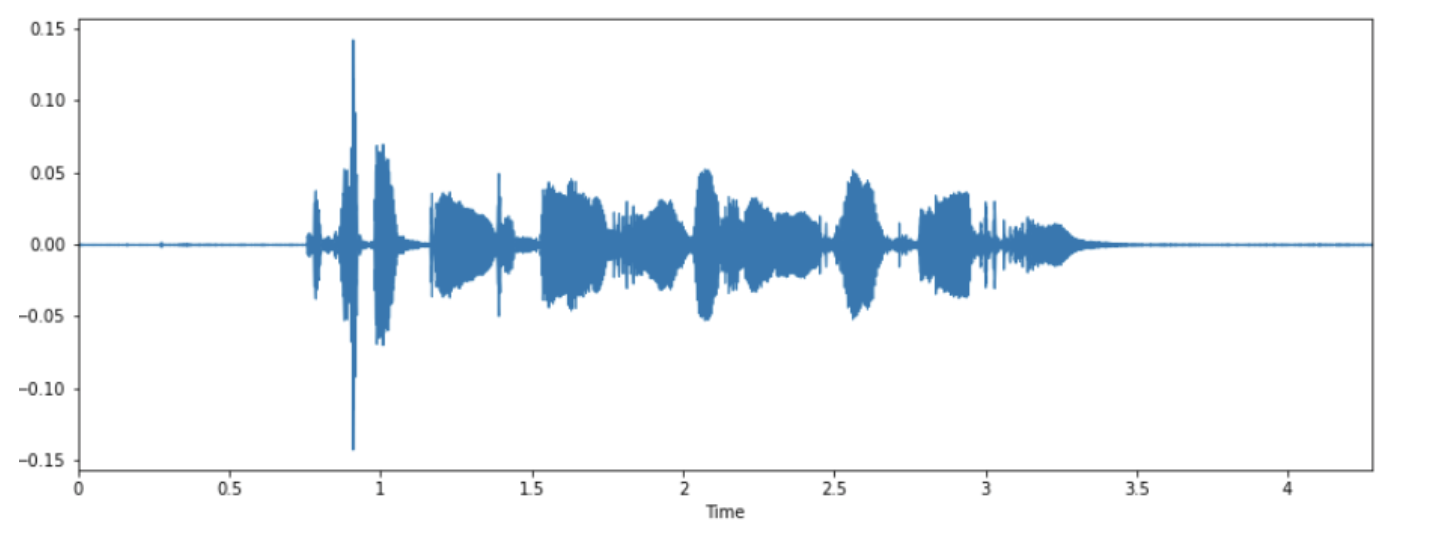
\includegraphics[width=0.70\textwidth]{audio_wave.png}
            \caption{Example of sound wave.}
            \label{fig:wave}
\end{figure}
\subsubsection{Resize to the same length}
We then resize all the audio samples to have the same length by either extending its duration by padding it with silence, or by truncating it. In our case audio samples is truncated.

\subsubsection{Data augmentation}
Next, we can do data augmentation on the raw audio signal by applying different techniques. Most relevant are applied: i)\textit{Time Stretch}: randomly slow down or speed up the sound, ii)\textit{Add Nois}: add some random values to the sound, iii) \textit{Time Shift: }shift audio to the left or the right by a random amount.

\subsubsection{Mel Spectrogram}
Deep learning models rarely take this raw audio directly as input. The common practice is to convert the audio into a \textit{Mel Spectrogram}. It captures the essential features of the audio and are often the most suitable way to input audio data into different models.
The spectrogram is a concise ‘snapshot’ of an audio wave and since it is an image, it is well suited to being input to CNN-based architectures developed for handling images. Spectrograms are generated from sound signals using Fourier Transforms. A Fourier Transform decomposes the signal into its constituent frequencies and displays the amplitude of each frequency present in the signal. It plots Frequency (y-axis) vs Time (x-axis) and uses different colors to indicate the Amplitude of each frequency. The brighter the color the higher the energy of the signal. 
\newline \newline
From the definition of Spectogram, it's possible to define mel Spectogram. It makes two important changes relative to a regular Spectrogram that plots Frequency vs Time. It uses the Mel Scale instead of Frequency on the y-axis and the Decibel Scale instead of Amplitude to indicate colors (\hyperref[fig:spectogram]{Figure~\ref*{fig:spectogram}})

\begin{figure}[h]
            \centering
            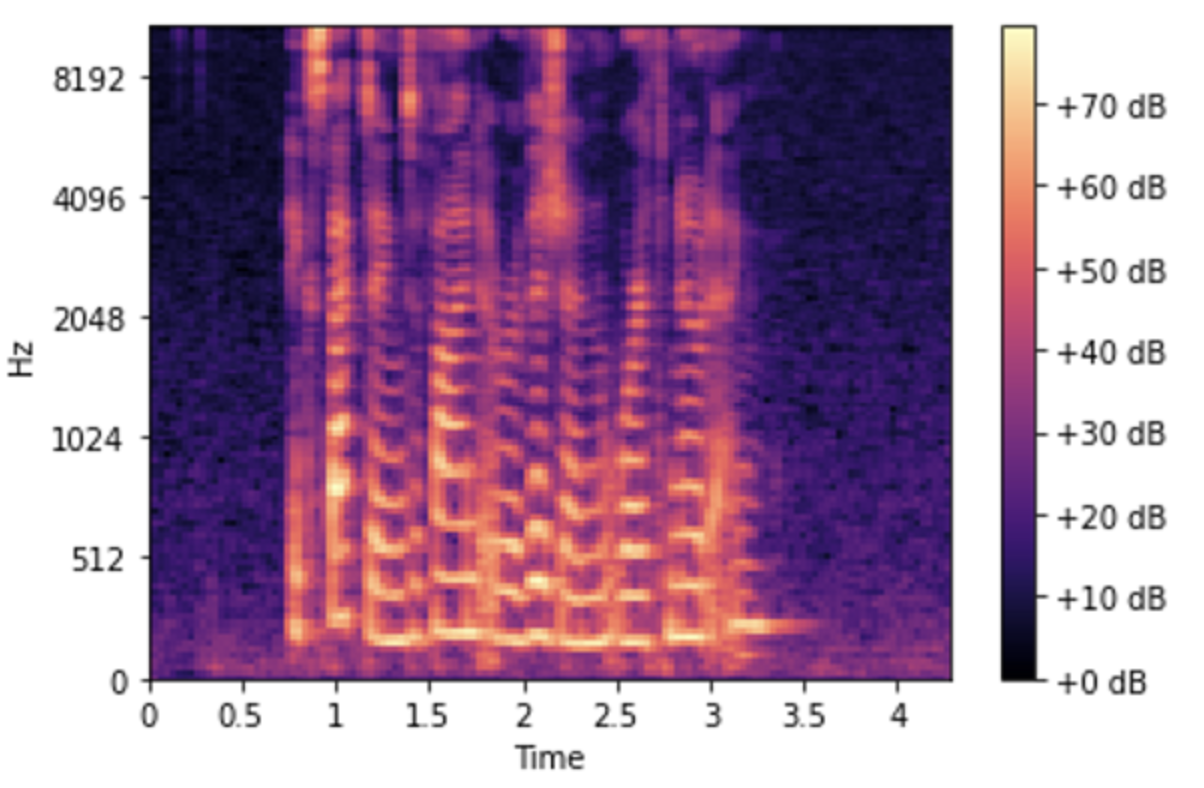
\includegraphics[width=0.70\textwidth]{mel-spectogram.png}
            \caption{Example of mel spectogram representation.}
            \label{fig:spectogram}
\end{figure}

After this overview on Audio classification and Audio processing we can introduce the thesis work.
First we downloaded and got ESC-50 dataset through specific API. Then we proceed with a preprocessing phase, performing previously defined steps in order to obtain data which are ready to use to reach the final goal: these data are used to create different Continual Learning Benchmarks based on different CL Scenario. All details are introduced in next chapters,

\chapter{Continual learning benchmark}
In this chapter we build on the knowledge of the framework Avalanche as introduced in \hyperref[chap5]{Chapter~\ref*{chap5}}, and go into greater detail in describing the work presented in this thesis.
The goal is to evaluate Continual learning strategies on a new benchmark based on ESC-50 dataset, about the relevant problem of Event Sound Classification; all dev steps are performed by taking advantage the functionalities of Avalanche, as described in the following sections. It implies to use Python language and Pytorch library for processing data. 
All activities and implementation that will be presented later are based on the dataset built from ESC-50 dataset, as explained in previous chapter.
\section{How build Continual Learning Benchmark for  Environment Audio Classification}
As described in \hyperref[chap5]{Chapter~\ref*{chap5}}, Avalanche library offers several modules. One of the most useful is Benchmark module. It allows to create a new benchmark from scratch using specific available functions.
Before seeing the actual implementation, it is necessary to make a premise and describe the various continual learning scenarios that we want to experiment. From the choice of the data type, we decided to explore Domain-Incremental and a Multi-Task-Incremental scenarios.
\newline \newline
A new class, from Avalanche, has been created in order to allow to create two different benchmarks based on previously introduced CL scenario. In next sections we'll focus on implementation details of them.
\subsection{Benchmark: task incremental scenario}
Avalanche provides different Benchmark generators (\hyperref[chap5]{Chapter~\ref*{chap5}}) that allow to create easily and quickly new benchmark starting from a new stream of data, for our experiment we use ESC-50 dataset (after cleaning and preprocessing phases).  In order to generate this type of benchmark, a function named \textit{nc\_benchmark} has been used. As described by its name, this is the high-level benchmark instances generator for the "New Classes" (NC) case (\hyperref[chap-332]{Section~\ref*{chap-332}}) . Given a sequence of train and test datasets creates the continual stream of data as a series of experiences. Each experience will contain all the instances belonging to a certain set of classes and a class won't be assigned to more than one experience. In other words it splits all the available classes in a number of subsets equal to the required number of experiences. Patterns are then allocated to each experience by assigning all patterns of the selected classes. This means that the New Classes generator can be used as a basis to set up Task or Class-incremental learning benchmarks. In this case we proceed to create multi-task-incremental, setting some input parameters as  shown in the following picture. 
\\
Since ESC-50 dataset has 50 different classes, i.e. 50 different targets, we have decided to set the number of experience of this dataset to 10, so the benchmark will have 10 different task, each of them will have a different task-id in order to obtain a multi-task-incremental scenario. It's important to take in consideration that the number of classes must be divisible without remainder by the number of experiences.


\subsection{Benchmark: domain incremental scenario}
Based on the type of data, an alternative to what has just been said can certainly be the domain incremental scenario. In order to generate this type of benchmark, a function named \textit{ni\_benchmark} has been used. This is the high-level benchmark instances generator for the "New Instances" (NI) case (\hyperref[chap-332]{Section~\ref*{chap-332}}). Given a sequence of train and test datasets it creates the continual stream of data as a series of experiences. This generator splits the original training set by creating experiences containing an equal amount of patterns using a random allocation schema. The main intended usage for this generator is to help in setting up Domain-Incremental learning benchmarks. In this case we focus on a single-incremental scenario where the same task label is assigned to each incremental experience. In this way each experience can be considered as the same task, and each of them can have the same or different balancing of classes. As shown in following figure we choice to balance classes in each experience in order to generate a second benchmark based on domain incremental CL scenario.
\begin{pythoncode}
#import new class that allow to download and get ESC-50 Dataset
from benchmarks.dataset.esc50.esc50 import ESC50

#import avalanche benchmarks genetaros that allow to create 
#New Class and New Instance CL scenarios
from avalanche.benchmarks import ni_benchmark, nc_benchmark

#get train and test set from ESC-50. Trin test is also augmented.
train_dataset = ESC50(root= os.path.abspath(os.getcwd()),download =True, 
data_aug=True, train=True)
test_dataset = ESC50(root= os.path.abspath(os.getcwd()),download =True, 
data_aug=False, train=False)

#set number of experience for CL scnarios
n_experiences = 10

#create Multi-task incremental scenario from ESC-50 dataset. 
#'task_labels' = True allows to have a multi-task scenario.
task_incremental = nc_benchmark(
                        train_dataset=train_dataset,
                        test_dataset=test_dataset,
                        n_experiences=n_experiences,
                        task_labels=True,
                        seed=123,
                        fixed_class_order=None,
                        shuffle=True,
                        class_ids_from_zero_in_each_exp=True) 

#create Domain Incremental scenario from ESC-50 dataset. 
#'balance_experiences' = True allows to have a balancing of classes 
#in each experience.                        
domain_benchmark=  ni_benchmark(
                        train_dataset=train_dataset,
                        test_dataset=test_dataset,
                        n_experiences=n_experiences,
                        task_labels=True,
                        seed=123,
                        shuffle=True,
                        balance_experiences = True)
    
\end{pythoncode}
\captionof{pythoncode}{Example of new benchmarks created by Avalanche library}

\vspace{5mm}
Summarizing we created two different Continual Learning benchmarks based on two CL scenarios. These two are the base of our experiments. We'll adopt different CL strategies on these two benchmark, focusing on their evaluation: in this way we proceed to explore the Continual Learning on new field, such as the Environment Sound Classification. The idea of choosing two continual learning scenarios and not only one, is based on having a method of comparison in the context of continual learning that offers currently several research areas .


\section{Deep architectural model: CNN}
Following the definition and creation of the benchmarks, we proceed to define a suitable deep architectural model in order for the type of data we will need to manage. Avalanche offers pre-defined and ready-to-use models, but as introduced before this library is built for image classification; for this reason a new deep neural network model is implemented that will be more appropriate to manage audio data. As explained in \hyperref[5-3]{Section~\ref*{5-3}}, this type of data can be processed in several ways and this depends also on how the input data is pre-processed. Since the streams of the data are represented through mel-spectograms, CNN-based architectures are all suited to process this type of input.
\newline \newline
In this section Convolution Neural Network basic notions are introduced with a brief summary of its basic implementation in thesis work.

\subsection{CNN: overview and properties}
CNNs are a particular type of neural networks, which use the convolution operation in one or more layers for the learning process. These networks are inspired by the primal visual system, and are therefore extensively used with image and video inputs. A CNN is composed by three main layers:


\begin{itemize}
    \item Convolutional Layer: The convolutional layer is the one tasked with ap- plying the convolution operation on the input. This is done by passing a A CNN Approach for Audio Classification in Construction Sites 3 filter (or kernel) over the matricial input, computing the convolution value, and using the obtained result as the value of one cell of the output matrix (called feature map); the filter is then shifted by a predefined stride along its dimensions. The filters parameters are trained during the training process.
    \item Detector layer: In the detector layer, the output of the convolution is passed through a nonlinear function, usually a ReLU function.
    \item Pooling layer: The pooling layer is meant to reduce the dimensionality of data by combining the output of neuron clusters at one layer into one single neuron in the subsequent layer.
\end{itemize}
The last layer of the network is a fully connected one (a layer whose units are connected to every single unit from the previous one), which outputs the probability of the input to belong to each of the classes.


CNNs in a machine learning system show some advantages with respect to traditional fully connected neural networks, because they allow sparse interactions, parameters sharing and equivariant representations.

\subsection{Proposed CNN architecture}
The reasons why we used CNNs in our approach is due to the intrinsic nature of audio signals. CNNs are extensively used with images and, since the spectrum of the audio is an actual picture of the signal, it is straightforward to see why CNNs are a good idea for such kind of input, being able to exploit the adjacency properties of audio signals and recognize patterns in the spectrum images that can properly represent each one of the classes taken into consideration.

\begin{figure}[h]
            \centering
            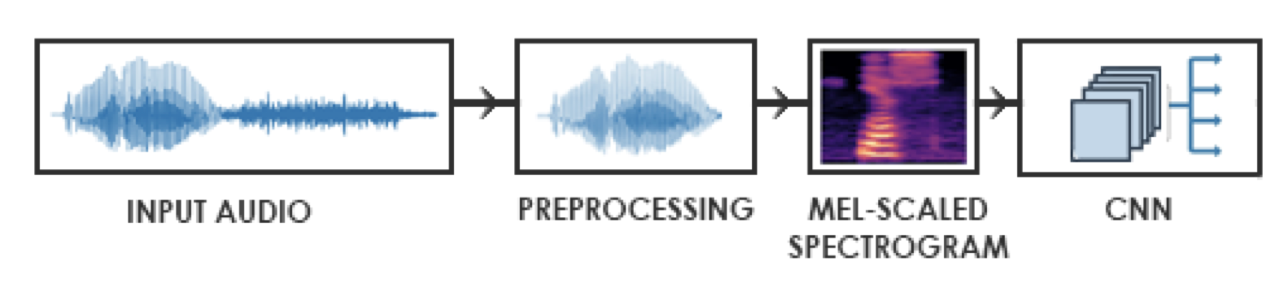
\includegraphics[width=0.90\textwidth]{audio_cnn.png}
            \caption{Framework for CNN-based audio classification.}
            \label{fig:cnn-audio}
\end{figure}

The proposed architecture consists in a DCNN composed of eight layers, that is fed with the mel spectrogram extracted from audio signals.
Then, we have five convolutional layers, followed by a dense fully connected layer and a final softmax layer that performs the classification over the classes.

All the layers employ a \textit{ReLu} activation function except for the output layers which uses a \textit{Sofmax} function. The optimizer chosen for the network is a \textit{SGD} optimizer, with the a learning rate set to 0.001 and a momentum equal to 0.9. Regarding the setting of other hyper-parameters, different strategies were adopted; they are detailed in next sections where continual learning strategies with specific Avalanche functions that allow to insert different hyper-parameters.

\section{Strategies adopted}
In this thesis work we showcase the flexibility of Avalanche for research, by applying some defined Continual learning strategies on a new type of data, so far not deepened: sound and audio streams, more specifically about Environment Sound Classification. We chose three different strategies in order to have a better overview on the behavior of Continual learning on audio classification, since its study on this field has not been very thorough until now.
From several strategies provided by Avalanche, three of them have been selected to be focused on these experiments: EWC (Elastic Weight Consolidation), Naive and Replay. To explore better the theoretical notions about these three algorithms, we refer you to \hyperref[chap-3-4]{Chapter~\ref*{chap-3-4}}.

We have chosen Elastic Weight Consolidation for several reasons, first of all its importance:at the time of writing the publication has been cited more than 2000 times (according to Google Scholar) and has had a significant impact on the CL scene as it has also been implemented in Avalanche for the supervised setting.
Then its usefulness in the topic of classifications; its way of applying the regularization could be very suitable in optimizing the continual learning on audio data such as our case in this work.

\vspace{5mm}
In order to obtain great and strong results, EWC are compared with Naive and Replay strategies that are considered two most robust, efficient and safe CL algorithm offered by Avalanche. All these three strategies, as explained previously are based on three different ways of acting; so it can be very interesting to understand which is the best and more efficient among them. 

In terms of Avalanche functions, they can be described as follow:
\begin{itemize}
    \item \textit{Naive}: the simplest (and least effective) Continual Learning strategy. Naive just incrementally fine tunes a single model without employing any method
    to contrast the catastrophic forgetting of previous knowledge.
    This strategy does not use task identities.
    \item \textit{EWC}: It computes importance of each weight at the end of training on current experience. During training on each minibatch, the loss is augmented
    with a penalty which keeps the value of the current weights close to the
    value they had on previous experiences in proportion to their importance
    on that experience. Importances are computed with an additional pass on the
    training set. This plugin does not use task identities.
    \item \textit{Replay}: It handles an external memory filled with randomly selected
    patterns and implementing `before\_training\_exp` and `after\_training\_exp`
    callbacks. 
    The `before\_training\_exp` callback is implemented in order to use the
    dataloader that creates mini-batches with examples from both training
    data and external memory. The examples in the mini-batch is balanced 
    such that there are the same number of examples for each experience.  
\end{itemize}



\newline \newline




\begin{pythoncode}

#import Avalanche strategies: EWC, Replay and Naive
from avalanche.training.strategies import EWC, Replay, Naive
#import custom deep model: CNN
from models.CNN import CNN
#import SGD optimization method
from torch.optim import SGD
#definition of loggers and CL metrics
from avalanche.logging import InteractiveLogger, WandBLogger
from avalanche.training.plugins import EvaluationPlugin
from avalanche.evaluation.metrics import forgetting_metrics, accuracy_metrics, 
loss_metrics, forward_transfer_metrics, bwt_metrics

#define deep model: CNN
model = CNN()

#define SGD optimization method
optimizer = SGD(model.parameters(), lr=0.001, momentum=0.9)

#define loss function as Cross Entropy
criterion = CrossEntropyLoss()

#definition of loggers
interactive_logger = InteractiveLogger()
config = wandb.config
wandb_logger = WandBLogger(project_name="tesi", run_name="replay_ni", 
                               config=config)
                               
#definition of EvaluationPlugin object with all metrics and loggers
eval_plugin = EvaluationPlugin(
                accuracy_metrics(minibatch=True, epoch=True, experience=True, 
                stream=True), 
                loss_metrics(minibatch=True, epoch=True, experience=True, 
                stream=True), 
                forgetting_metrics(experience=True, stream=True), 
                bwt_metrics(experience=True, stream=True),
                forward_transfer_metrics(stream=True),
                loggers=[interactive_logger, wandb_logger])
                
#define EWC strategy with previous defined parameters
cl_strategy_ewc = EWC(
            model, optimizer, criterion, ewc_lambda=0.4,
            train_mb_size=15, train_epochs=25, eval_mb_size=15,
            evaluator=eval_plugin, 
            eval_every = 0)

#define Naive strategy with previous defined parameters
cl_strategy_naive = Naive(model, optimizer, criterion, 
            train_mb_size=15, train_epochs=25, eval_mb_size=15,
            evaluator=eval_plugin, #it will contains logger for CL metrics
            eval_every = 0)

#define Replay strategy with previous defined parameters            
cl_strategy_replay = Replay( model, optimizer, criterion,
            train_mb_size=15, train_epochs=25, eval_mb_size=15,
            evaluator=eval_plugin, #it will contains logger for CL metrics
            eval_every = 0)

\end{pythoncode}
\captionof{pythoncode}{Example of definition of three different CL strategies using Avalanche. }
\vspace{5mm}
For each strategy, Avalanche allows to describe some parameters to manage better their functionality.The two most important features that are present in each algorithm are mini-batches and the epochs. From different values of these parameters, the time of training and execution and the global accuracy could be better or worst. In order to choose better these variables, more tests have been done. 

About mini-batches, we could define different values for mini batches during training and evaluation phase. As described in the following script, same value for both is decided, equal to 15.

Regarding train epochs, from several attempts, the decision has been to set it to 25.


As we can see in the script attached, in addition to the standard parameters that are previously defined (model, criterion and optimizer) there is evaluator parameter that allows to specify which metrics our strategy should take in consideration and how these metrics should be printed out, i.e the loggers. In terms of code, it accepts and object called \textit{evalutator\_plugin} that obtains relevant data from the training and eval loops of the strategy through callbacks. The plugin keeps a dictionary with the last recorded value for each metric. Metrics and loggers that are used in thesis work are represented in the figure and they will be discussed in next chapter. Just to introduce them, metrics used in this project are accuracy, loss, BWT, forgetting and several system metrics, while loggers to print out and store metric results are \textit{WandBLogger} and (using W&B tool) and \textit{InteractiveLogger} that easily print out results during training and testing execution.

Finally, for this work, another EWC parameter is used: \textit{ewc\_lambda}  hyperparameter to weigh the penalty inside the total loss. The larger the lambda, the larger the regularization. It has been set to 0.4 .


Summarizing, now we are ready to use all strategies on both different scenarios previously created. 

\section{Training phase}
In this section training phase is discussed, where all strategies previously introduced are tested on two different type of Continual learning scenario: Domain Incremental and Multi Task Incremental; these scenario are built from ESC-50 dataset about Environment Sound Classification. 

In the following script there is a resume about how a continual learning strategy is trained on a specific scenario based on audio dataset.
\vspace{2mm}
\begin{pythoncode}


from avalanche.training.strategies import EWC, Replay, Naive
from torch.optim import SGD
from benchmarks.classic.splitESC50 import CLEsc50
from models.CNN import CNN

splitEsc =  CLEsc50(n_experiences=10, seed=123,                       
                    return_task_id=True,balance_experiences=True,shuffle=True)

...
... # definition of EWC parameters
...

cl_strategy_ewc = EWC(
            model, optimizer, criterion, ewc_lambda=0.4,
            train_mb_size=15, train_epochs=25, eval_mb_size=15,
            evaluator=eval_plugin, #it will contains logger for CL metrics
            eval_every = 0)


train_stream = splitEsc.train_stream
test_stream = splitEsc.test_stream

print('Starting experiment...')
results = []
for experience in train_stream:
    print("Start of experience: ", experience.current_experience)
    print("Current Classes: ", experience.classes_in_this_experience)

    cl_strategy.train(experience,
                        eval_streams=[test_stream])
    print('Training completed')

    print('Computing accuracy on the whole test set')
    results.append(cl_strategy.eval(test_stream))
    #print(cl_strategy.eval(scenario.test_stream))
    print('**************************************')

\end{pythoncode}
\captionof{pythoncode}{Training of EWC strategy on multi task incremental scenario based on ESC-50 dataset. }
\vspace{5mm}

First we should define a Continual Learning scenario, Multi task incremental with ten experiences as in figure; then we proceed to create a CL strategy setting all required parameters, EWC in the example.

From scenario previously created, we can obtain train and test stream with which we work for training and evaluation phases. For each experience in train stream we use the method "train" provided by strategy object that allows to train all data in that stream, in the mean time all chosen metrics are printed out. 
After training on specific task, we proceed to evaluate the whole test stream: so for each experience we got metric results for all test set. Each time we obtain different results, in according to the amount of trained data. All results during training phase will be explored and presented in next chapters.


\part{Evaluating Continual Learning strategies}

\chapter{Continual learning metrics}
The continual learning training protocol is the straightforward extension of what is normally done in classic machine learning on fixed training set to a sequence of multiple training batches. However, in particular cases, shuffling the order of the training batches over multiple runs may be needed for assessing stability of the proposed algorithms. More complex cross-validation techniques may be also conceived but are not very common in current CL research.
\section{Proposed metrics}
For an evaluation of deep learning model, we can assume to have access to a series of test sets $T B_i$ over time. The purpose is to assess the performance of our hypothesis $h_i$ as well as to evaluate if it is representative of the knowledge that should be learned by the correspondent training batch $B_i$.
However, as discussed in \cite{lopez}, a different granularity of the evaluation at the task level can as well be achieved by having the same test batch for many $B_i$. For simplicity, in the description metrics described below we assume to have access to each $T B_i$, and define the cumulative training set and cumulative test set respectively as:

\begin{equation}
                B_i^C = \bigcup_{i=1}^{i-1}{B_i}, \quad   T B_i^C = \bigcup_{i=1}^{i-1}{T B_i}
\end{equation}
\vspace{5mm}

The absence of consensus in evaluating continual learning algorithms and the almost exclusive focus on forgetting motivated to propose a more complete set of implementation independent metrics accounting for several aspects we believe have practical consequences that can be considered essential in the deployment of real AI systems that learn continually: accuracy or performance over time, forward and backward knowledge transfer, memory overhead as well as computational efficiency.
\vspace{5mm}

In order to provide bounds to each metric, it's mapped to a [0, 1] range, so that its optimal value is given by its maximization. This is done to maintain meaning of the proposed aggregating $CL_{score}$ metric, and allow to evaluate CL strategies with respect to several aspects, rank them from best to worst, and build weighting schemes according to constraints.
\vspace{5mm}

Focusing on all characteristic of Continual Learning Benchmark, described in \hyperref[chap:3]{Chapter~\ref*{chap:3}}, there are several interesting aspects that could be monitored to explore better the performance of different CL strategies. Following list shows all aspects and concept that are the basis of the definition of all metrics that will be defined below.

\begin{itemize}
    \item Performance on current experience
    \item Performance on past experiences
    \item Performance on future experiences
    \item Resource computation (Memory, CPU, GPU, Disk usage)
    \item Data efficiency
    \item Execution time
    \item Model size growth
\end{itemize}

From these points, we explore all different Continual Learning metrics present in current literature (citazioni).
\subsection{Accuracy}
Given the train-test accuracy matrix $R \in R^{n×n}$, which contains in each entry $R_{i,j}$ the test classification accuracy of the model on task $t_j$ after observing the last sample from task $t_i$ \cite{lopez}, Accuracy (A) considers the average accuracy for training set $B_i$ and test set $TB_j$ by considering the diagonal elements of R, as well as all elements below it (see \hyperref[tab:acc]{Table~\ref*{tab:acc}}):

\begin{equation}
                 ACC = \frac{\sum_{i=1}^{n}{R_{i,j}}}{\frac{n(n+1)}{2} } 
\end{equation}
\vspace{5mm}

Accuracy was originally defined to asses performance of the model at the end of the last task \cite{lopez}. This new way to define Accuracy in CL was born by the idea to take into account the performance of the model at every timestamp i in time better characterizes the dynamic aspects of CL. The same idea is applied also for two new metrics, described below: FWT and BWT.

\begin{table}[h!]
            \centering
            \begin{tabular}{ |c| c c c| }
                \hline
               R & $Te_1$ & $Te_2$ & $Te_3$ \\
                \hline \hline
                 $Tr_1$ & $R^\ast$ & $R_{ij}$ & $R_{ij}$ \\
                \hline
                 $Tr_2$ & $R_{ij}$ & $R^\ast$ & $R_{ij}$ \\
                \hline
                 $Tr_3$ & $R_{ij}$ & $R_{ij}$ & $R^\ast$ \\
                \hline 
            \end{tabular}
            \caption{Elements in R accounted to compute the Accuracy.
            $R^\ast = R_{ii}$, $Tr_i$ = training, $Te_i$ = test tasks}
            \label{tab:acc}
        \end{table}
        
Matrix $R \in R ^{N×N}$ contains in each entry $R_{i,j}$ the test classification accuracy of the model on task j after observing the last sample from task i. N is the number of tasks; here for simplicity we make the number of distributions n equal to N . \hyperref[tab:acc]{Table~\ref*{tab:acc}} shows the elements in the accuracy matrix used for each metric for an example matrix of N = 3 tasks. $R^\ast = R_{ij}$ coincides with the (normally) optimal accuracy right after using training set $Tr_i$ and testing on test set $Te_i$ .
\subsection{Loss}
In the context of an optimization algorithm, the function used to evaluate a candidate solution is referred to as the objective function.

We may try to maximize or minimize the objective function; it means that we are searching for a possible solution that has the highest or lowest score respectively.

Normally, through neural networks, we try to to minimize the error. As such, the objective function is often referred to as a cost function or a loss function and the value obtained by the loss function is referred to as simply “loss.”

A lot of the loss functions are available for different purposes. The most relevant are the following:
\begin{itemize}
    \item \textit{MSE (Mean Squared Error): }it creates a criterion that measures the mean squared error (squared L2 norm) between each element in the input x and target y.
    \item \textit{Cross Entropy Loss:} it computes the cross entropy loss between input and target. It is useful when training a classification problem with `C` classes.
    \item \textit{ L1 loss:} it creates a criterion that measures the mean absolute error (MAE) between each element in the input x and target y.
\end{itemize}

For the thesis work Cross Entropy Loss is used as loss function and we'll evaluate the model also this metric,as described in the following chapter. 
\subsection{Backward Transfer (BWT)}
Backward Transfer measures the influence that learning a task has on the performance on previous tasks \cite{lopez}. The reason appears when an agent needs to learn in a multi-task or data stream setting. The lifelong capacity to both improve and not degrade performance are important and should be evaluated throughout its lifetime. It can be defined as the accuracy computed on $TB_i$ right after learning Bi as well as at the end of the last task on the same test set. (\hyperref[tab:acc]{Table~\ref*{tab:acc}}). Here, as in the accuracy metric, we expand it to consider the average of the backward transfer after each task:

\begin{equation}
                 BWT = \frac{\sum_{i=2}^{N}{\sum_{j=1}^{i-1}{(R_{i,j} - R_{j,j})}}}{\frac{n(n+1)}{2} } 
\end{equation}

In order to give more importance to two semantically different concepts, BWT is broken into two different clipped terms: the negative value, called forgetting and it can be defined as $1 -  min(BWT, 0)$; the positive value, called properly positive Backward Transfer $BWT^+$ and it can be defined as $max(BWT, 0)$
\vspace{5mm}
\subsection{Forward Transfer (FWT)}
It measures the influence that learning a task has on the performance of future tasks. Following the spirit of the previous metrics we modify it as the average accuracy for the train-test accuracy entries $R_{i,j}$ above the principal diagonal of R, excluding it (\hyperref[tab:acc]{Table~\ref*{tab:acc}}). Forward transfer can occur when the model is able to perform zero-shot learning. We therefore redefine FWT as:

\begin{equation}
                 FWT = \frac{\sum_{i < j}^{n}{R_{i,j}}}{\frac{n(n+1)}{2} } 
\end{equation}

\subsection{System metrics}
Previous metrics are based on the evaluation of the performance of the model, monitoring each experience focusing on the behavior among them.
In deep neural network, system performance is another relevant concept to take in consideration during evaluation of specific model. In continual learning, where the effort of a model is higher and more expensive, it becomes more important to monitor several performance of the system where the model is trained and evaluated. The following list shows some relevant system metrics that can be used in the evaluation phase over a continual learning strategy:
\begin{itemize}
    \item RAM usage
    \item CPU usage
    \item GPU usage
    \item Memory usage
    \item Disk Usage
    \item Model size efficiency (MS)
    \item Computational efficiency (CE)
 
\end{itemize}

Also these metrics can be represented and evaluated through all different experience or as an average at the end of the last experience.
\section{CL metrics by Avalanche}
The performance of a CL algorithm should be assessed by monitoring several features of the computation, previously described. The evaluation component has a wide set of metrics to evaluate experiments.
Avalanche’s main idea is to separate the issues of what to monitor and how to monitor it: the evaluation components provides support for the former through the metrics, while the logging module fulfills the latter. Metrics don't specify the format of their output and how it should be displayed, while loggers do not alter metrics results. Metrics can work even without a logger: the strategy’s train and eval methods return a dictionary with all the metrics logged during the experiment.


A small script is sufficient to monitor a large set of metrics: accuracy, loss, confusion matrix, catastrophic forgetting,  timing, CPU/disk/ram/GPU usage and Multiply and Accumulate (which measures the computational effort of the model’s forward pass in terms of floating point operations). Every metric is composed by a standalone class and a set of plugin classes aimed at emitting metric values on specific instants during training and evaluation phases.

\subsection{Stand-alone metrics}
Stand-alone metrics are used autonomously of all Avalanche features. Each metric can be applied through a simple Python object.
\subsection{Plugin metrics}
Plugin metrics can be integrated into the Avalanche training and evaluation methods. They release a curve composed by different values at different moments over time.
\subsection{Evaluation Plugin}
Evaluation Plugin is the responsible for the orchestration of both plugin metrics and loggers. It has the role to get metrics outputs and forward them to the loggers during training and evaluation phases.

Avalanche allow also to create an own metric based on different characteristic over a continual learning scenario.



\chapter{Results metrics}
\label{results}
In this chapter, experiments assessing the continual learning strategies on Environment Sound Classification are discussed. As described many times in previous chapters, Avalanche library is used to perform these experiments; for each different CL metric we explore results in two different scenarios: Multi task incremental and Domain incremental. Different CL strategies (EWC, Replay and Naive) are compared in same plots. All eval analysis are performed by loggers and metrics components provided by Avalanche.

In next sections, each metric is explored with some graphs and following explanations of its representation. In order to obtain optimal and robust results, each experiment has been done through five runs; all graphs are the representation of the average of this several executions for related metric.

\section{Accuracy evaluation}
The first metric we consider is Accuracy. It is the most popular metric for all machine learning and deep learning models; in this case we explore it in two different point of view (only for multi task incremental scenario):
\begin{itemize}
    \item At first we consider the accuracy on test stream, only for the tasks that are already trained. In other words, accuracy is calculated in each iteration, after every training on different experience and we take in consideration the average of the accuracy calculated on some tasks.
    \item The second way is simpler and it is referred to a global accuracy. After each iteration, accuracy is calculated by the mean among all accuracy performed by all task, also those are not already trained in train stream during training phase.
\end{itemize}


\subsubsection{Multi task incremental scenario}
\begin{figure}[!h]
   \begin{minipage}{0.48\textwidth}
     \centering
     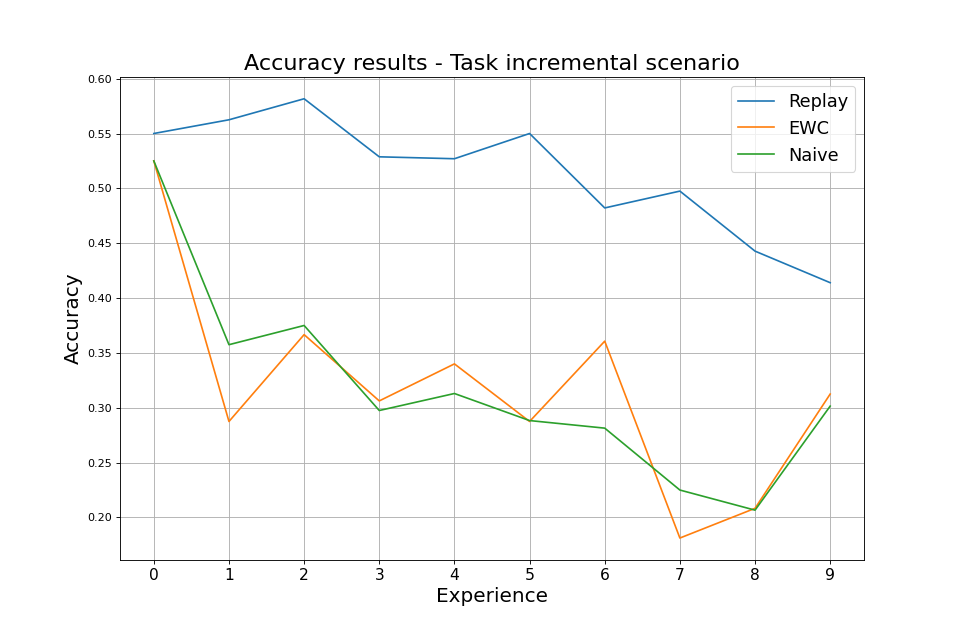
\includegraphics[width=1.1\linewidth]{overview_accuracy_before_nc.png}
     \caption{Accuracy metric calculated on previously task trained - multi line chart. Multi task incremental scenario}\label{Fig:92}
   \end{minipage}\hfill
   \begin{minipage}{0.48\textwidth}
     \centering
     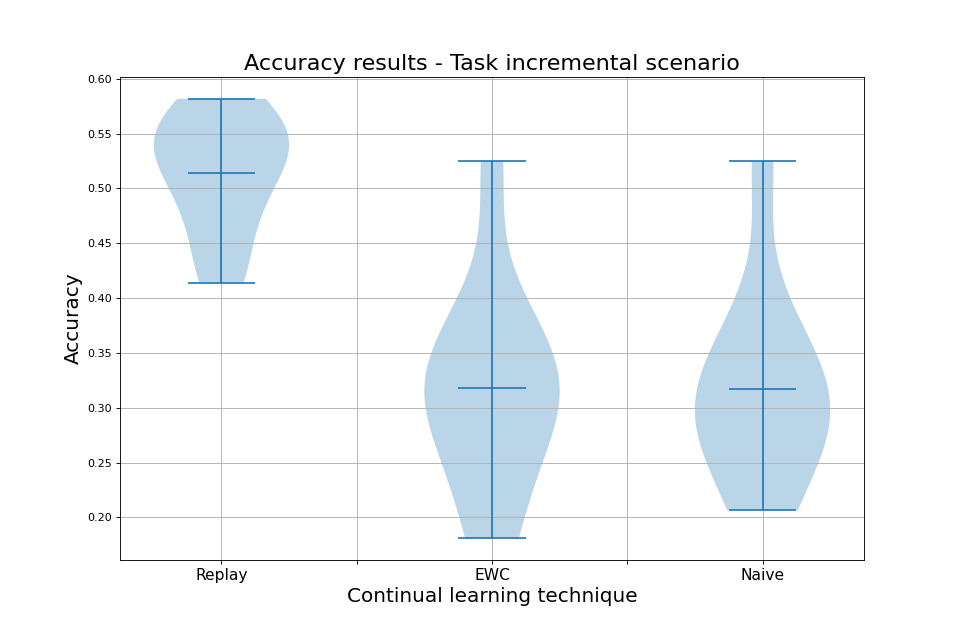
\includegraphics[width=1.1\linewidth]{overview2_accuracy_before_nc.png}
     \caption{Accuracy metric calculated on previously task trained - violin plot. Multi task incremental scenario}\label{Fig:91}
   \end{minipage}
\end{figure}

From graphs in \hyperref[Fig:92]{Figure~\ref*{Fig:92}} and \hyperref[Fig:91]{Figure~\ref*{Fig:91}} we can see the behavior of the accuracy during all evaluation phases. It's refer to the first case explained before. In x axes there are our ten experience and y axes represent the value of the accuracy calculated after every experience by a mean among all previous tasks. For example (in Replay case), after experience 4 we got an accuracy equal 0.53. This value is calculated by the average of first five task (from 0 to 4) in test stream after experience 4 is trained in train stream.

These two plots compare all three CL strategies introduced in previous chapters: in first plot we compare them with a multi line chart (different color for each algorithm), in second graph we plot them by using a violin plot and each algorithm is represented distinctly. 

It is quite easy to understand by these two representations, the best CL strategy, focusing only on accuracy, is significantly Replay. EWC and Naive algorithm has same similar results. For all three strategies the accuracy starts from approximately 0.55 and then they decrease quickly, except for Replay. For the first six task it has value higher 0.5 threshold, until descending to 0.43 as final value. Other two strategies reach the same final accuracy, equal to 0.30; their behavior is enough similar but not exactly the same. It's visible from the violin plot. In Naive algorithm all Accuracy value are more concentrated to the final values than EWC.
\begin{figure}[!h]

     \centering
     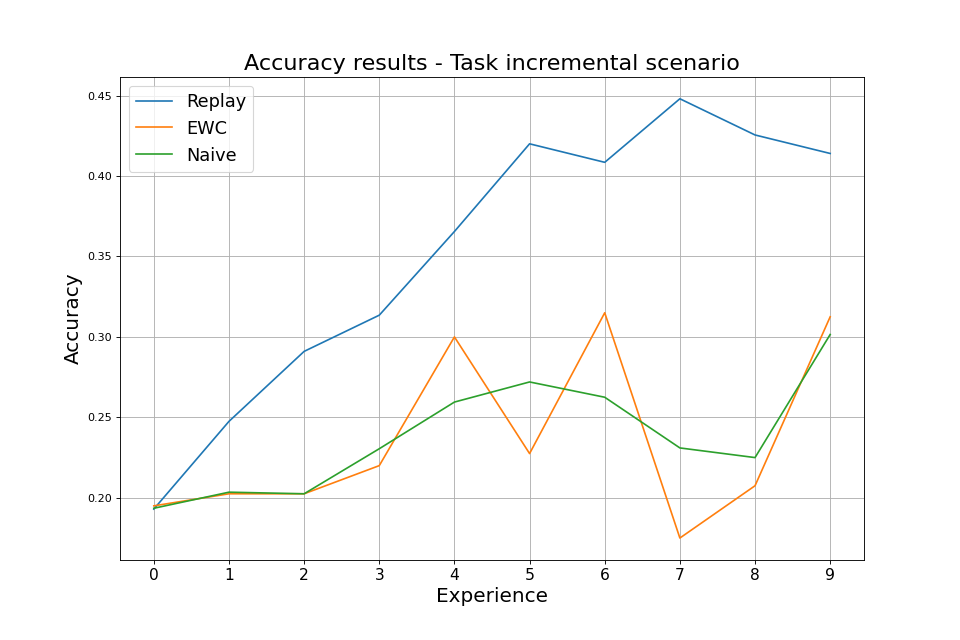
\includegraphics[width=0.60\textwidth]{overview_accuracy_nc.png}
     \caption{Global Accuracy metric calculated on last task on whole test set - multi line chart. Multi task incremental scenario}\label{Fig:93}
   
\end{figure}

This multi line chart graph (\hyperref[Fig:93]{Figure~\ref*{Fig:93}}) is the representation of the global accuracy, explained in the second point in the previous explanation; it compare all three different CL strategies. Accuracy is calculated focusing on all test stream. For example, after training of experience 5, accuracy is calculated by the average of accuracy in all task on the whole test set. It's evident for all algorithm the behavior of this metric is growing among all experiences and also here the best strategy is Replay. Moreover we can see that the final value for each algorithm is the same final accuracy for all of them in previous algorithm (after last experience the accuracy is calculated on whole test stream).
\subsubsection{Domain incremental scenario}

\begin{figure}[!h]
  
     \centering
     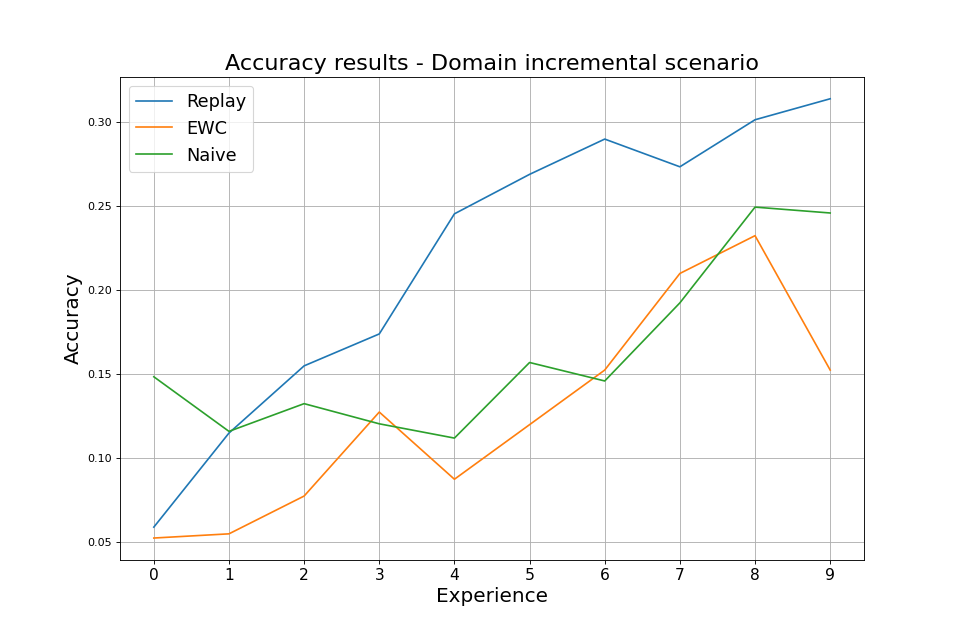
\includegraphics[width=0.60\textwidth]{overview_accuracy_ni.png}
     \caption{Global Accuracy metric calculated on last task on whole test set - multi line chart. Domain incremental scenario}\label{Fig:94}
   
   
\end{figure}
In Domain Incremental scenario (\hyperref[Fig:94]{Figure~\ref*{Fig:94}}), it's important to remember tasks identities are unknown during evaluation phase. We focus on global accuracy as in the last graph.
Also in this scenario the accuracy behavior is better in replay (reaching final value 0.33) respect to Naive and EWC. These global results are worst than task incremental scenario where all three algorithm have better values. 

From a point of view of the accuracy, the performance of the CL strategies on a benchmark based on an Environment Audio Classification is better in a multi task incremental scenario respect to a Domain incremental scenario. In all graphs, it's easy to see that the better algorithm (regardless of the scenario) is Replay.


\section{Loss evaluation}
The second metric we consider is Loss. It is calculated by the loss function used in the strategies; for simplicity, we used the same function named "\textit{Cross Entropy Loss}" for all CL algorithms. As it was done for the accuracy, also here loss metrics has been monitored by two point of view (see previous section to see again this categorization).
\subsubsection{Multi task incremental scenario}
\begin{figure}[h]
   \begin{minipage}{0.48\textwidth}
     \centering
     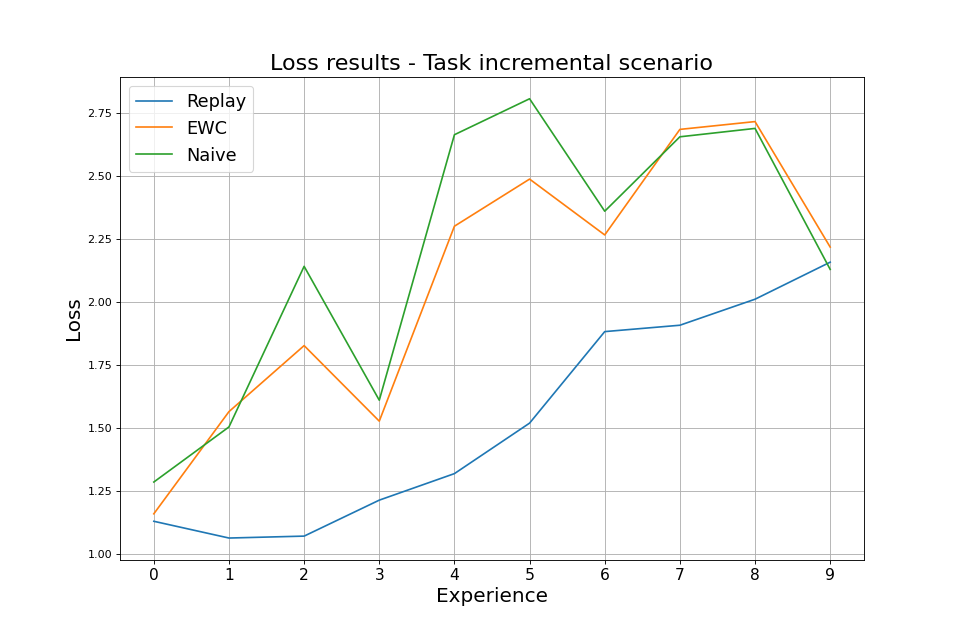
\includegraphics[width=1.1\linewidth]{overview_loss_before_nc.png}
     \caption{Loss metric calculated on previously tasks trained - multi line chart. Multi task incremental scenario}\label{Fig:95}
   \end{minipage}\hfill
   \begin{minipage}{0.48\textwidth}
     \centering
     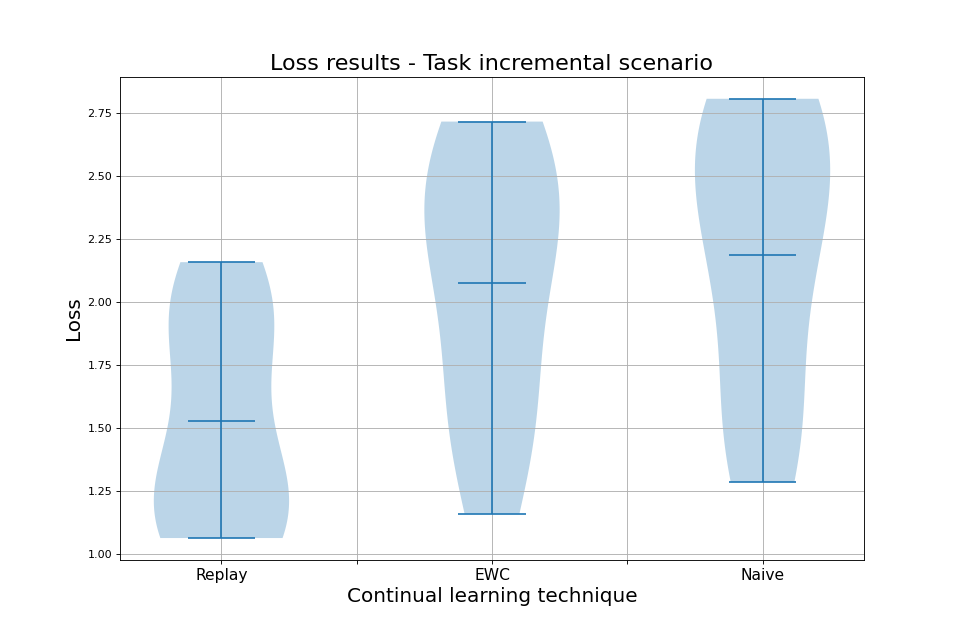
\includegraphics[width=1.1\linewidth]{overview2_loss_before_nc.png}
     \caption{Loss metric calculated on previously task trained - violin plot. Multi task incremental scenario}\label{Fig:96}
   \end{minipage}
\end{figure}

From these graphs, \hyperref[Fig:95]{Figure~\ref*{Fig:95}} and \hyperref[Fig:96]{Figure~\ref*{Fig:96}}, the behavior of the loss during all evaluation phases is represented. In x axes there are our ten experience and y axes represent the value of the loss calculated after every experience by an average among all previous tasks. For example (in Naive case), after experience 4 we got a loss equal 2.6. This value is calculated by the average of first five task (from 0 to 4) in test stream after training of experience 4.

EWC, Naive and Replay behaviors, about Loss metric, are represented with these two plots: multi line chart and violin plot.

Lower loss value means a better performance of the model. As for the accuracy, also for loss metric, the best CL strategies on task incremental scenario is Replay. After each experience, this value is lower than other strategies that are very similar. However the final loss (after 10 experiences) is the same for all algorithms.

In this regard, it is evident that for all strategies, loss value assumes always a growing value. It is caused by training of a part of train stream larger and larger. Just remember that in this case, after each experience the loss is calculated by the mean of previous tasks.

From second plot, it's possible to notice that Replay strategy assume loss value more concentrated to the final value than other two algorithm.

\begin{figure}[!h]

     \centering
     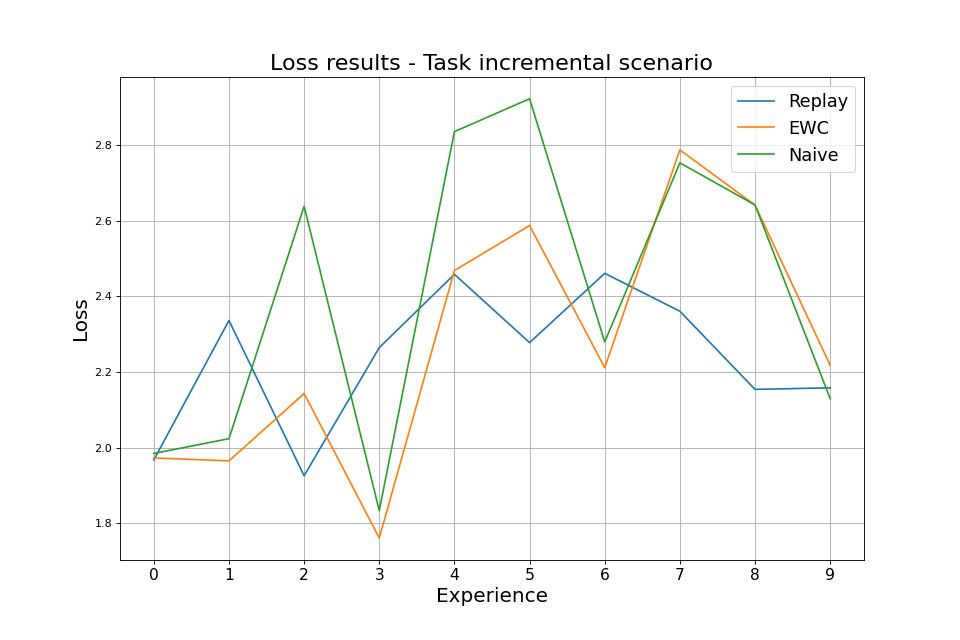
\includegraphics[width=0.60\textwidth]{overview_loss_nc.png}
     \caption{Global Loss metric calculated on last task on whole test set - multi line chart. Multi task incremental scenario}\label{Fig:97}
   
\end{figure}
In this \hyperref[Fig:97]{Figure~\ref*{Fig:97}} Loss is calculated focusing on all test stream. For example, after training of experience 5, loss is calculated by the average of loss in all task on the whole test set. It's evident for all algorithm the behavior of this metric is very unstable among all experiences; there is no evident best strategies, they start and finish in the same point with high curves. 

\subsubsection{Domain incremental scenario}

\begin{figure}[h]
  
     \centering
     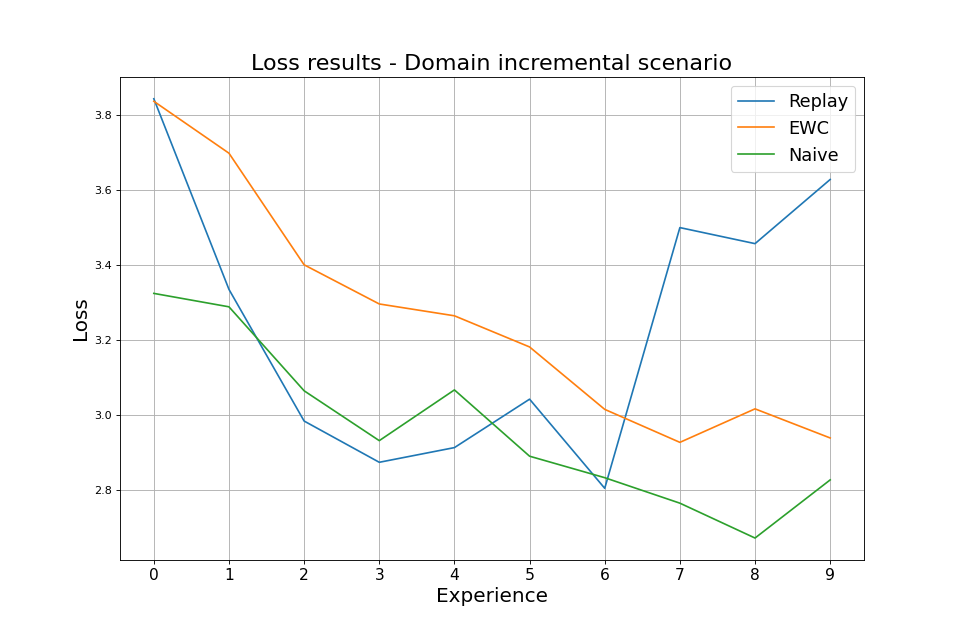
\includegraphics[width=0.60\textwidth]{overview_loss_ni.png}
     \caption{Global Loss metric calculated on last task on whole test set - multi line chart. Domain incremental scenario}\label{Fig:98}
   
   
\end{figure}
In \hyperref[Fig:98]{Figure~\ref*{Fig:98}} we focus on global loss for the Domain Incremental scenario.
In this case the loss behavior is particular: until sixth experience the best strategy turns out to be Replay, but in following tasks, loss grows quickly reaching 3.5. In Naive and EWC the behavior is more regular, there is a constant degrowth until to get better value than Replay, equal to 2.9. 

These global results are worst than task incremental scenario where all three algorithm have better values. 

\section{Forgetting evaluation}
Forgetting can be considered the most important concept in continual learning literature. As explained in \hyperref[chap:3]{Figure~\ref*{chap:3}}, catastrophic forgetting is the main issue that occurs in CL approach. Forgetting metrics is calculated from BWT value, it's simple the negative values that BWT can assume. When BWT get values below zero, it means that our strategy comes across the catastrophic phenomenon. 
Summarizing, when forgetting metric get values near zero, the performance of CL algorithm is very better.

Following plots show this metric that it's performed after each experience through an average among all tasks already trained.

\subsubsection{Multi task incremental scenario}
\begin{figure}[!ht]
   \begin{minipage}{0.48\textwidth}
     \centering
     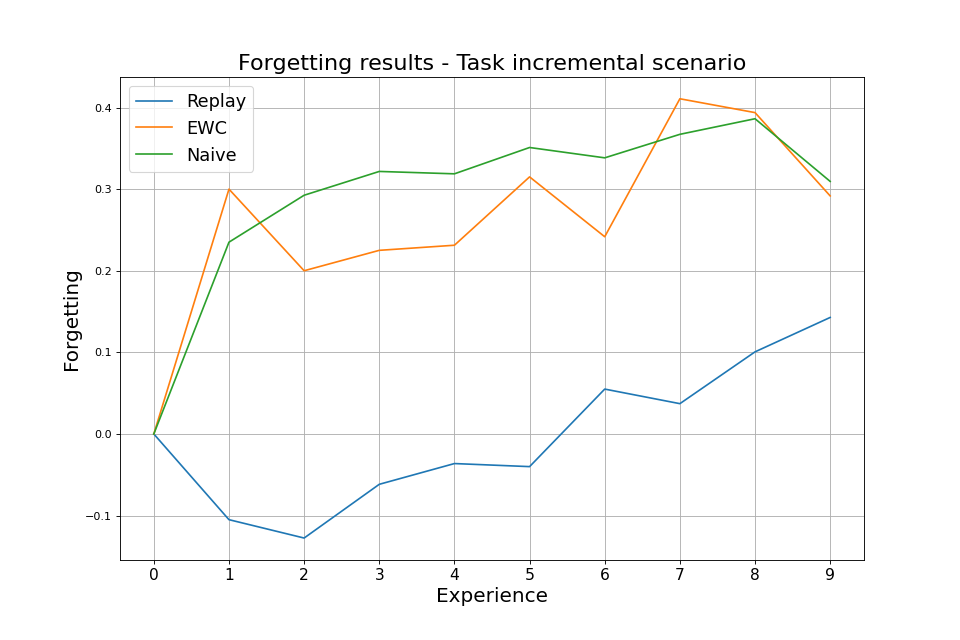
\includegraphics[width=1.1\linewidth]{overview_forgetting_nc.png}
     \caption{Forgetting metric calculated on previously tasks trained - multi line chart. Multi task incremental scenario}\label{Fig:99}
   \end{minipage}\hfill
   \begin{minipage}{0.48\textwidth}
     \centering
     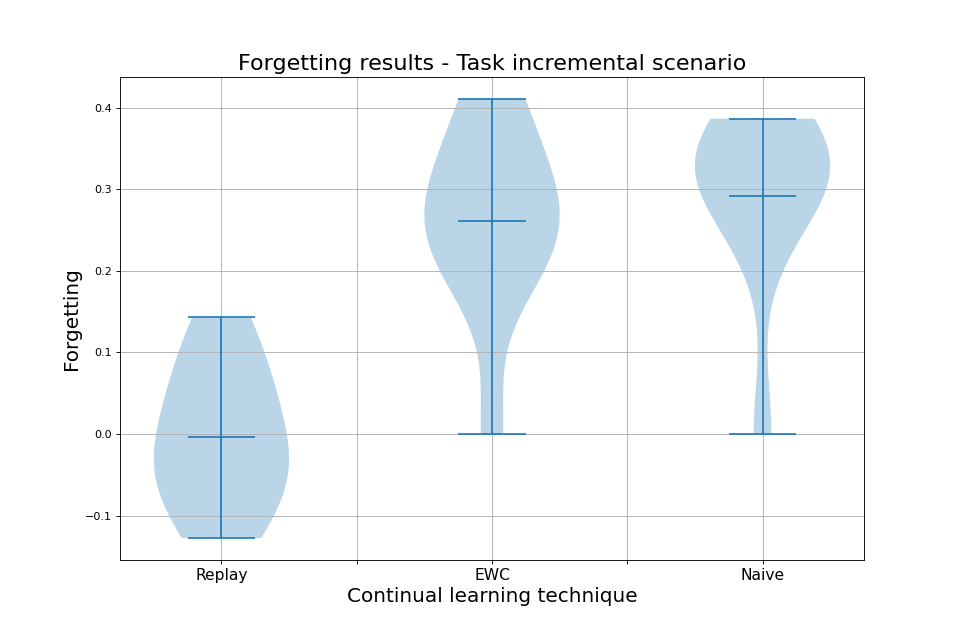
\includegraphics[width=1.1\linewidth]{overview2_forgetting_nc.png}
     \caption{Forgetting metric calculated on previously task trained - violin plot. Multi task incremental scenario}\label{Fig:100}
   \end{minipage}
\end{figure}

From these two graphs (\hyperref[Fig:99]{Figure~\ref*{Fig:99}} and \hyperref[Fig:100]{Figure~\ref*{Fig:100}}) we can see the behavior of the forgetting during all evaluation phases. 
In x axes there are our ten experience and y axes represent the value of the forgetting calculated after every experience by a mean among all previous tasks. 
For example (in Replay case), after experience 6 we got a forgetting equal to 0.05. This value is calculated by the average of seven five task (from 0 to 6) in test stream after training of experience 6. 
For multi task incremental scenario, the situation is very clear: Replay is the best strategy that gets values near 0 during almost all experience. In all algorithm there is a growth of this metric during all tasks, starting obviously from 0 in first task. In Naive and EWC there is more forgetting with an average near to 0.3 while Replay overcomes 0.1 threshold after last experience.


\subsubsection{Domain incremental scenario}
Following figures ((\hyperref[Fig:101]{Figure~\ref*{Fig:101}} and \hyperref[Fig:102]{Figure~\ref*{Fig:102}}) show the behavior of the forgetting metric in domain incremental scenario. For all strategies there is no catastrophic forgetting because this metric assumes always value below zero. Replay strategy gets better performance because the forgetting is lower but these performance are good also in other two algorithm. 
\begin{figure}[!h]
   \begin{minipage}{0.48\textwidth}
     \centering
     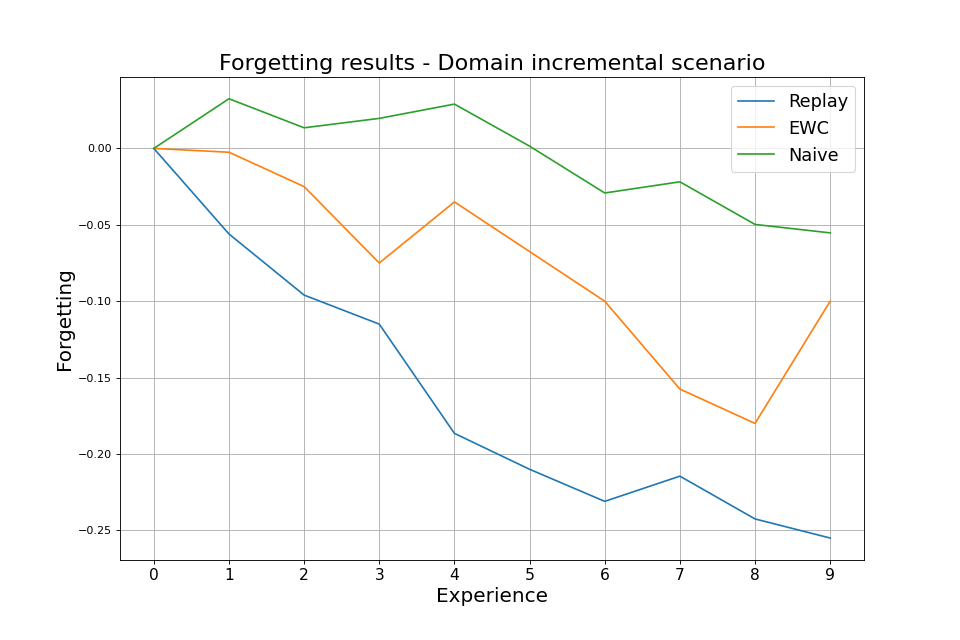
\includegraphics[width=1.1\linewidth]{overview_forgetting_ni.png}
     \caption{Forgetting metric calculated on previously tasks trained - multi line chart. Domain incremental scenario}\label{Fig:101}
   \end{minipage}\hfill
   \begin{minipage}{0.48\textwidth}
     \centering
     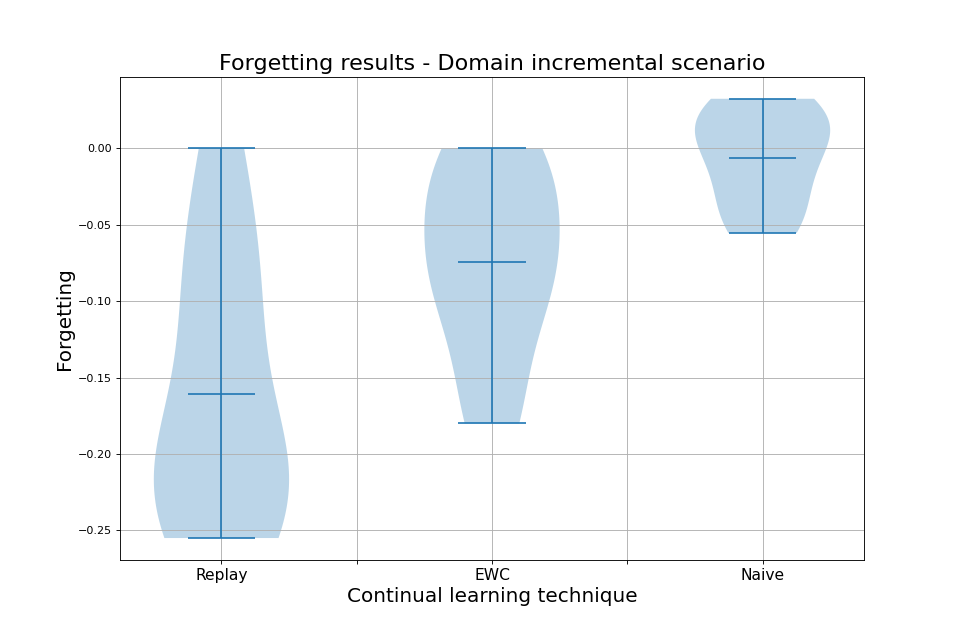
\includegraphics[width=1.1\linewidth]{overview2_forgetting_ni.png}
     \caption{Forgetting metric calculated on previously task trained - violin plot. Domain incremental scenario}\label{Fig:102}
   \end{minipage}
\end{figure}



Summarizing, focusing only on forgetting metric, all considered CL strategies have better performance in Domain incremental scenario respect to task incremental one. In other words the phenomenal of catastrophic forgetting is not present when we use CL strategies on a benchmark based on environment audio classification


\section{Backward Transfer (BWT) evaluation}
Backward Transfer (BWT) is the most important metric we explored and we get it as focal point for the evaluation of the experiment.
As described in previous chapter, BWT can assume negative and positive values and consequently it an be decomposed in two sub-metric. In this case when we talk about BWT, we refer to a global metric that can assume positive and negative values; in other words when there is negative values, it means that there is a forgetting and it should be present also in exploring forgetting metrics ( see previous section). A nearest value to zero means a better performance of CL strategy. As for the previous metrics, the following plots will show the behavior of the BWT in task incremental and domain scenarios.

\subsubsection{Multi task incremental scenario}
In these graphs (\hyperref[Fig:103]{Figure~\ref*{Fig:103}} and \hyperref[Fig:130]{Figure~\ref*{Fig:130}}), it is represented the evaluation of CL strategies, focusing on Backward Transfer metric. 
In x axes there are our ten experience and y axes represent the value of the bwt calculated after every experience by a mean among all previous tasks. For example, after experience 6 BWT value, during Replay algorithm, assumes -0.05 score and it is calculated by the average of this metric in first seven experience (from zero to six); in this particular case it means that after six experience we have a bit forgetting between task 5 and task 6.
\begin{figure}[h]
   \begin{minipage}{0.48\textwidth}
     \centering
     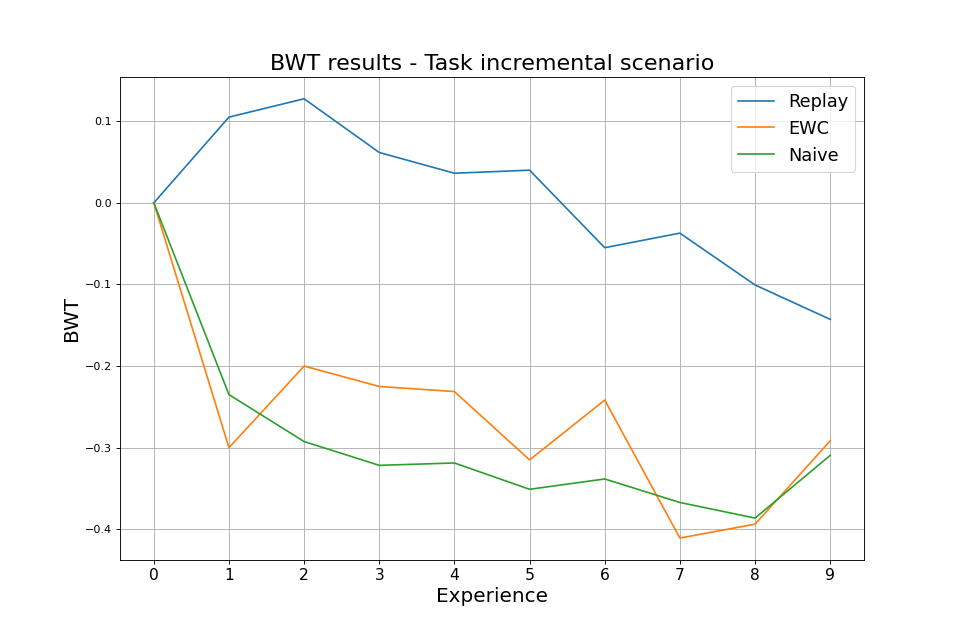
\includegraphics[width=1.1\linewidth]{overview_bwt_nc.png}
     \caption{BWT metric calculated on previously tasks trained - multi line chart. Multi task incremental scenario}\label{Fig:103}
   \end{minipage}\hfill
   \begin{minipage}{0.48\textwidth}
     \centering
     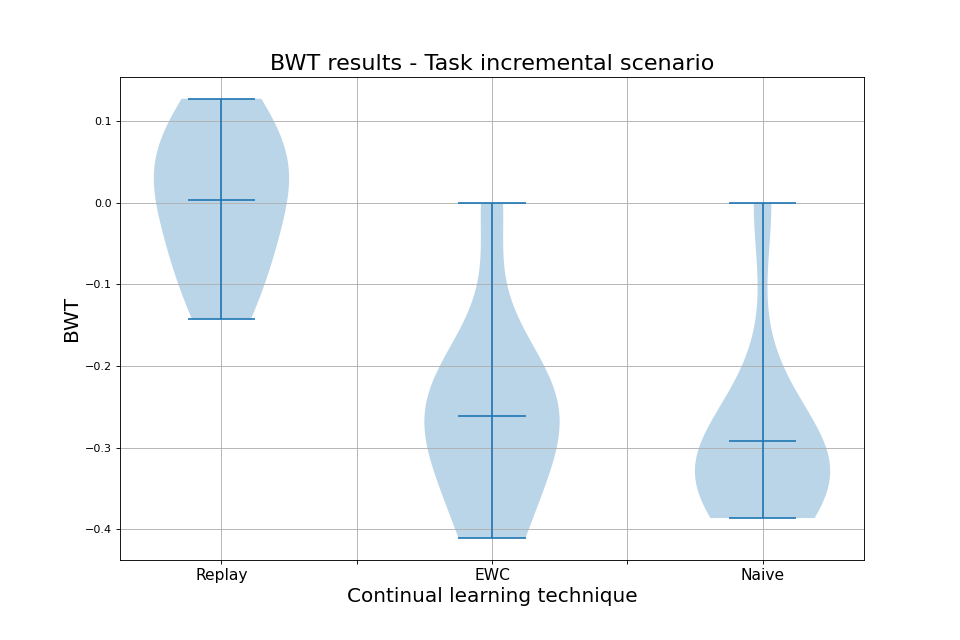
\includegraphics[width=1.1\linewidth]{overview2_bwt_nc.png}
     \caption{BWT metric calculated on previously task trained - violin plot. Multi task incremental scenario}\label{Fig:130}
   \end{minipage}
\end{figure}


Globally the behavior of BWT show the best performance of Replay strategy, while Naive and Elastic Weight Consolidation have a similar trend with slightly better for Naive strategy in last tasks.
Also for this metric, the best CL algorithm is Replay. It starts with great performances without forgetting until sixth experience and it finishes with -0.13 value that means there is a bit catastrophic forgetting phenomenon. When we explored forgetting metrics we have noticed also that in the last task there was a bit about it.
In violin plot, concentration of all average bwt after all task is represented. BWT is the technique with more concentration and balancing respect to final value. EEWC and Naive seems to be not very balanced.
\subsubsection{Domain incremental scenario}

\begin{figure}[h]
   \begin{minipage}{0.48\textwidth}
     \centering
     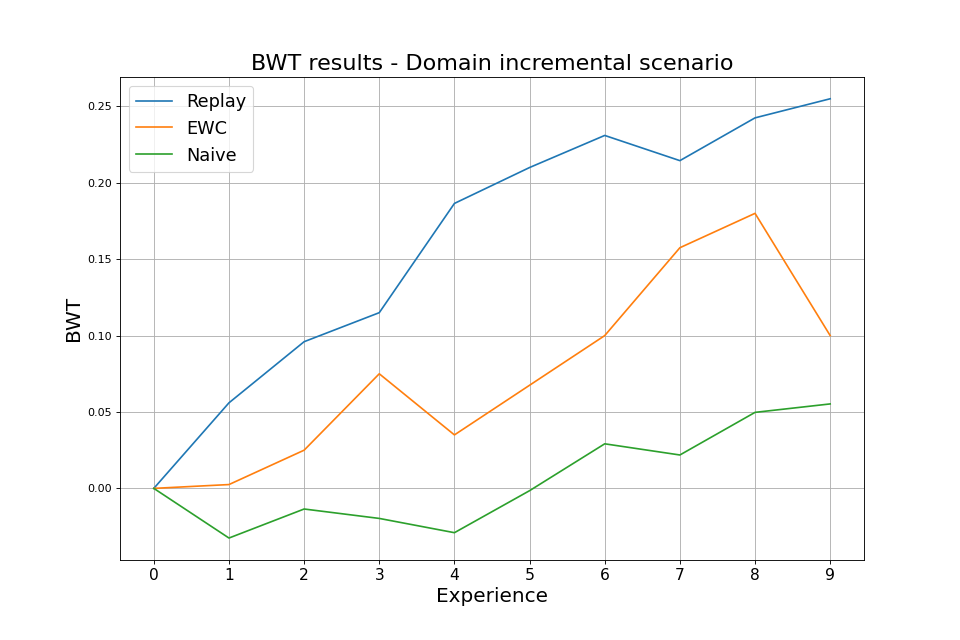
\includegraphics[width=1.1\linewidth]{overview_bwt_ni.png}
     \caption{BWT metric calculated on previously task trained - violin plot. Domain incremental scenario}\label{Fig:116}
   \end{minipage}\hfill
   \begin{minipage}{0.48\textwidth}
     \centering
     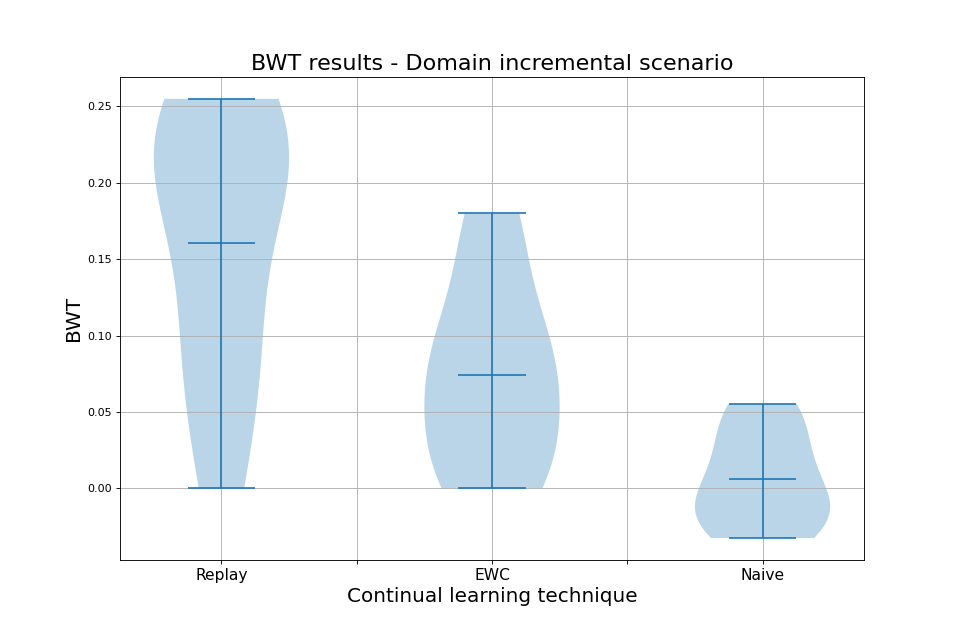
\includegraphics[width=1.1\linewidth]{overview2_bwt_ni.png}
     \caption{BWT metric calculated on previously task trained - violin plot. Domain incremental scenario}\label{Fig:117}
   \end{minipage}
\end{figure}
In Domain Incremental scenario (\hyperref[Fig:116]{Figure~\ref*{Fig:117}} and \hyperref[Fig:108]{Figure~\ref*{Fig:108}}), the behavior of BWT metric is quite better than task incremental. During all CL strategies adopted, there is no forgetting and we can see from the first graph that bwt is never below zero. Despite the three strategies have good performances under this point of view, replay has better behavior, reaching higher value equal to 0.27, even if during all task this strategy assume irregular set of values, from 0.0 to 0.27 (second graph).

By sum up, Replay is the best strategy for both scenarios and domain incremental seems to be the scenario where we got better performances among all CL algorithms.

\section{System metrics evaluation}
During an evaluation of Continual Learning strategy can be very interesting to monitor several system metric.
Avalanche allows to configure a new logger with WandB tool (Weight and Biases tool) through logger component.

Weights \& Biases is the machine learning platform for developers to build better models faster. Use W\&B's lightweight, interoperable tools to quickly track experiments, version and iterate on datasets, evaluate model performance, reproduce models, visualize results and spot regressions, and share findings with colleagues.

In the following sections, the evaluation of continual learning strategies has been done analysing several system metrics with WandB logger. It automatically logs system metrics every 2 seconds, averaged over a 30 second period.

\subsection{CPU usage}
CPU is important, for running prerequisites to run deep learning, such as importing data, data cleansing, visualization, statistics, loading data to GPU and so on.
If your CPU is weak, it can only feed as few data as possible thus cant keep up with your powerful GPU. Ideally Deep Learning training systems should have CPU with maximum number of processing cores to handle more work to catch up with a GPU.
In the following graphs, CPU usage metrics is represented for both scenarios; this metric is shown by the percentage of system CPU used by the CL strategy during training and evaluation phases.  In x axis there is the timeline (in minutes) and in the y axis there is the CPU usage represented in percentage. All three different CL algorithms are reported with three different colors.
\subsubsection{Multi task incremental scenario}
\begin{figure}[!h]
  
     \centering
     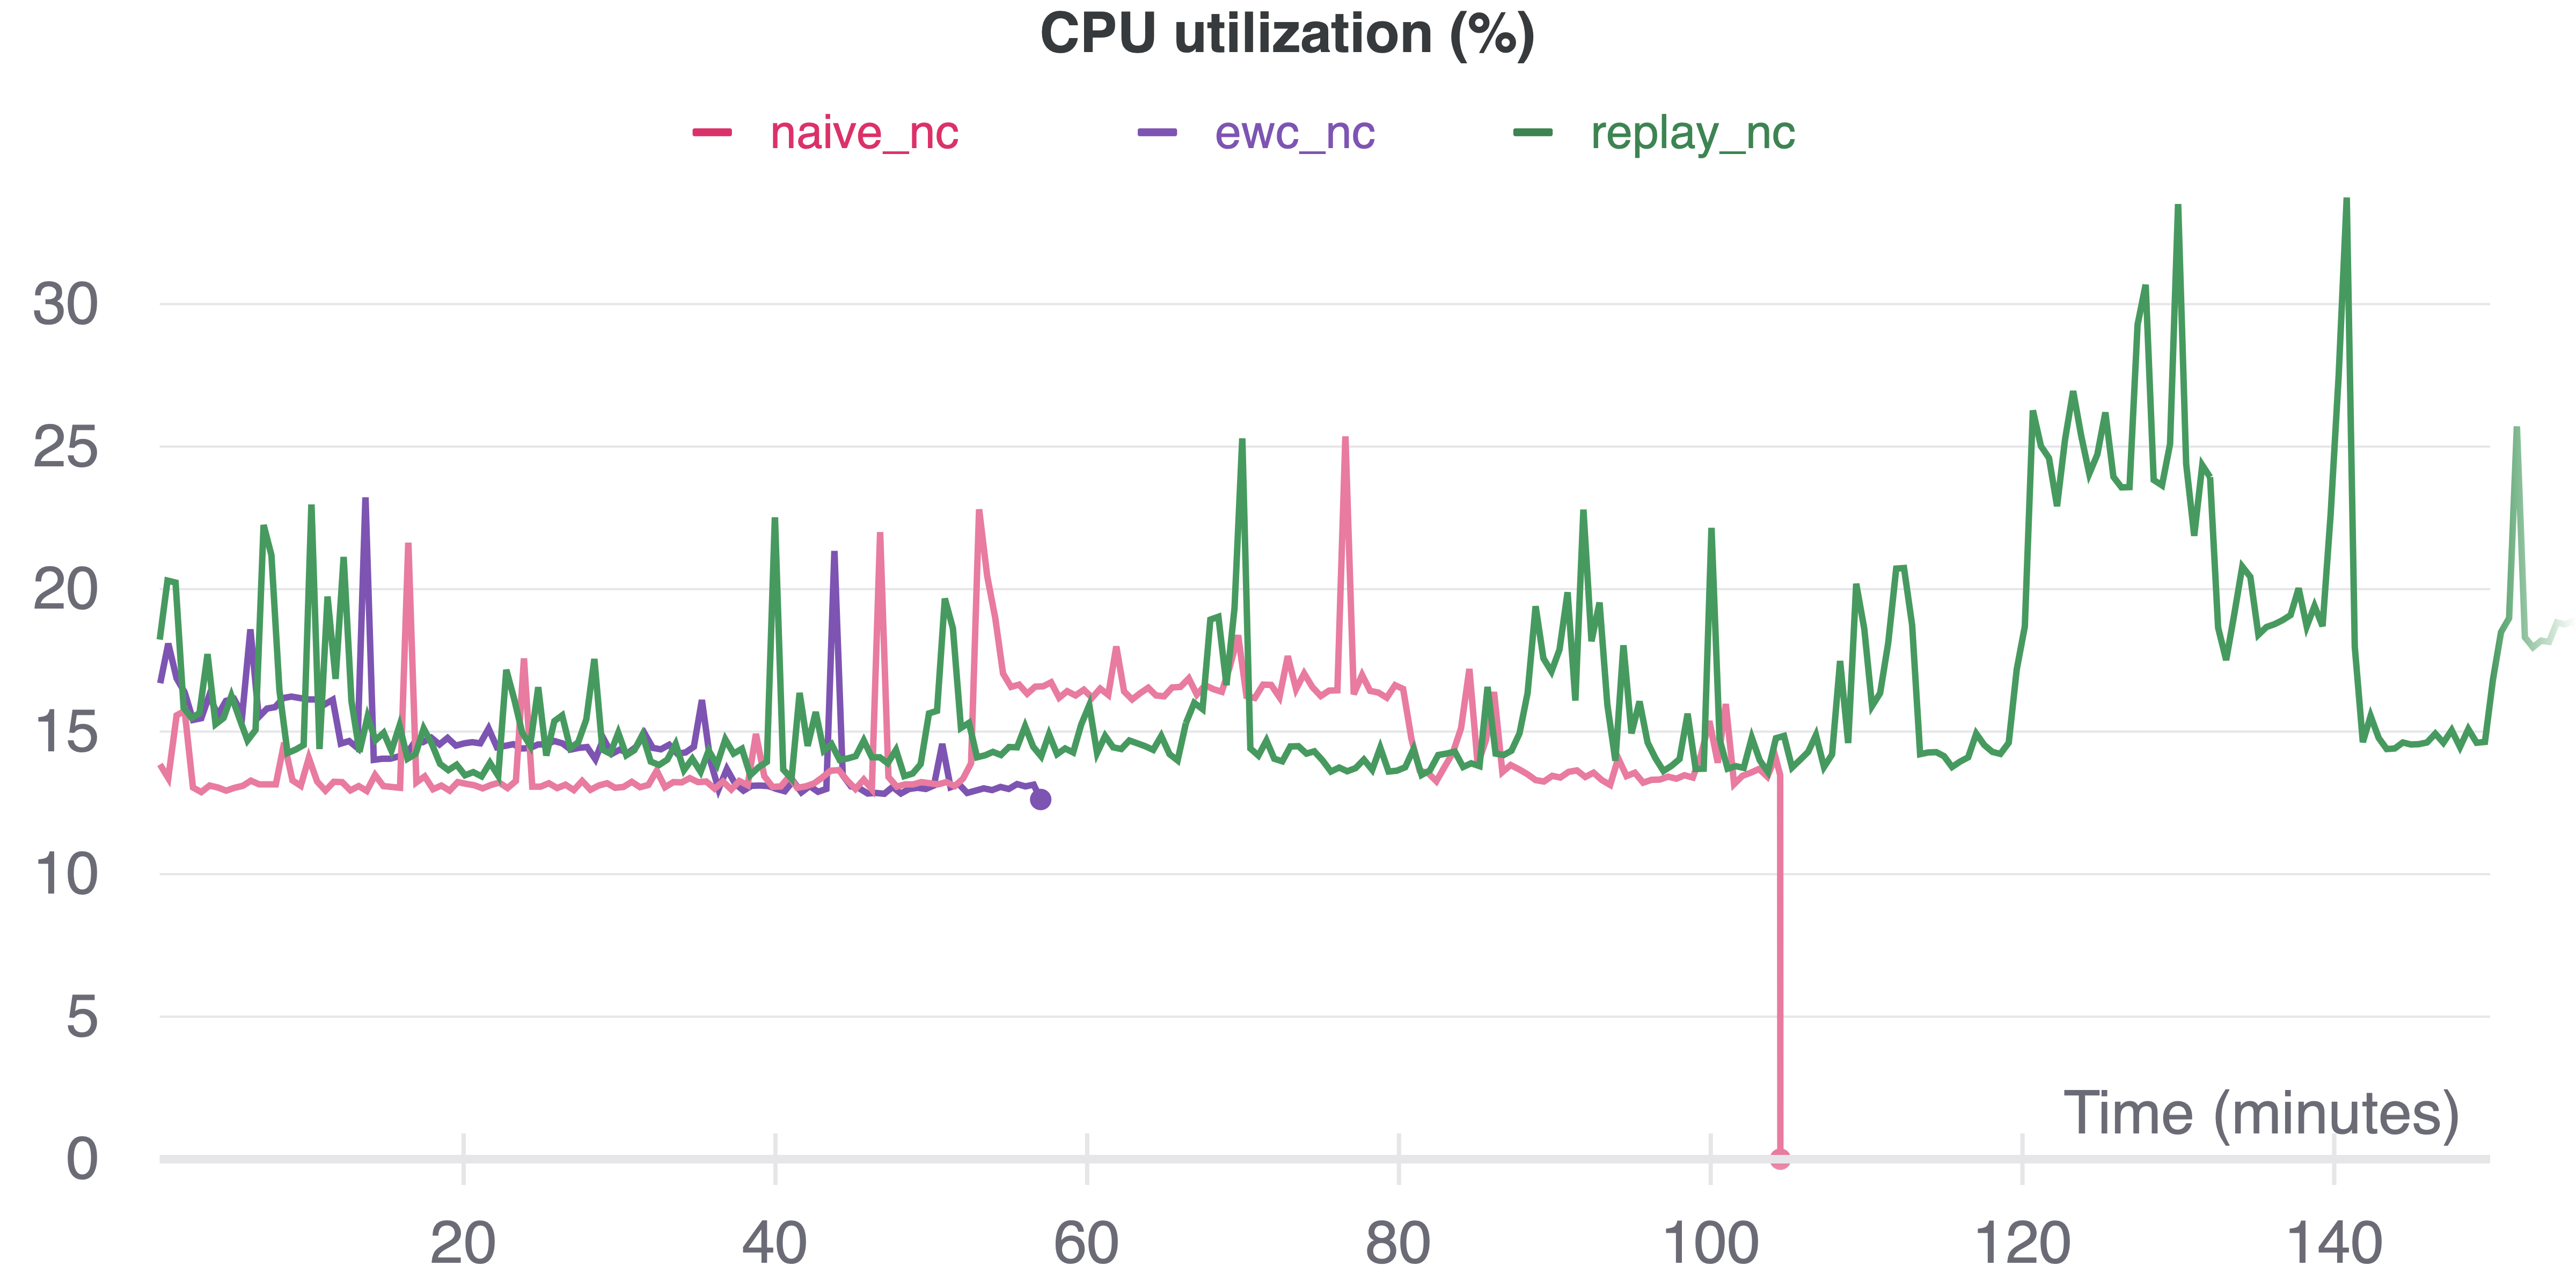
\includegraphics[width=0.60\textwidth]{overview cpu utilization nc.png}
     \caption{CPU usage - multi line chart. Multi task incremental scenario}\label{Fig:104}
   
   
\end{figure}
In this first case (\hyperref[Fig:104]{Figure~\ref*{Fig:104}}), Replay strategy needs to more CPU to complete their processes. This is traceable by the fact that this algorithm needs more time to be executed, for this reason the maximum CPU utilization (over 30\%) is present in last minutes (from 100 to 140) while Naive and EWC finish their process in less time and their curves have a similar behavior. Although, all three CL strategies don't need a big amount of CPU to complete their execution; the range of usage is between 15\% and 30\%.

\subsubsection{Domain incremental scenario}
In Domain Incremental scenario, the situation is quite different (\hyperref[Fig:105]{Figure~\ref*{Fig:105}}). Although Replay needs more time to be executed, in this case it needs less CPU. All three algorithms have a similar behavior, with an average of CPU consuming equal to 17\% . We can say that EWC and Naive consume more CPU in relation to their execution time.
\begin{figure}[!h]
  
     \centering
     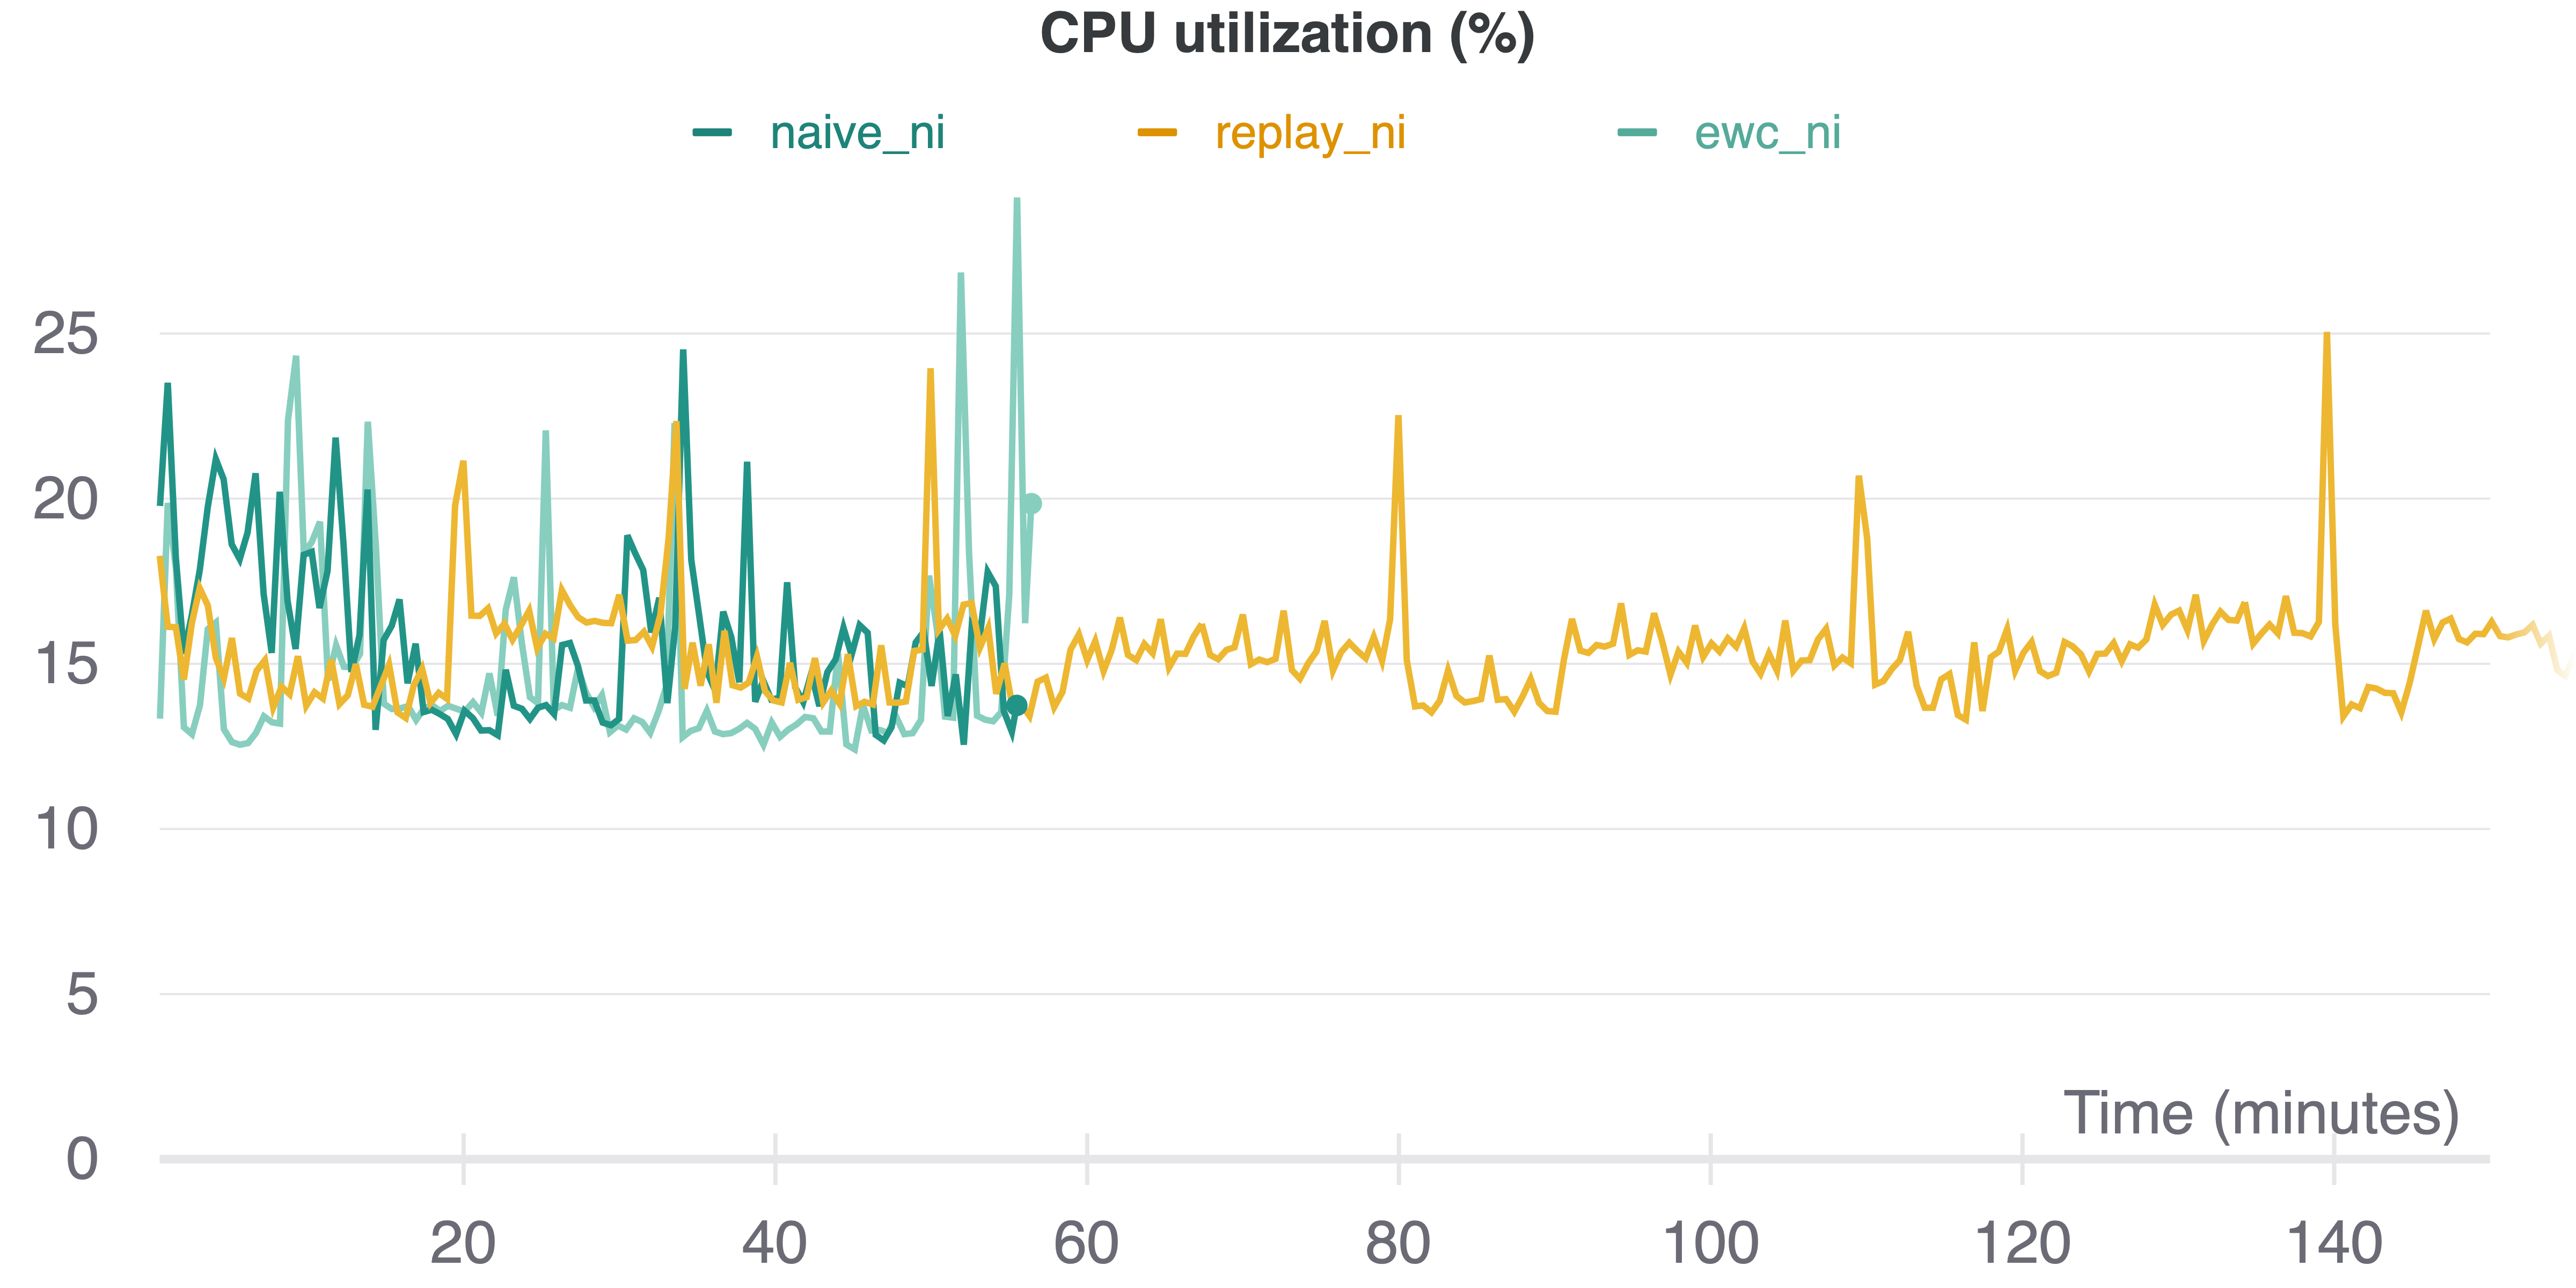
\includegraphics[width=0.60\textwidth]{overview cpu utilization ni.png}
     \caption{CPU usage - multi line chart. Domain incremental scenario}\label{Fig:105}
   
   
\end{figure}


\subsection{Disk usage}
Disk usage (DU) refers to the portion or percentage of computer storage that is currently in use. It contrasts with disk space or capacity, which is the total amount of space that a given disk is capable of storing. Disk usage is often measured in kilobytes (KB), megabytes (MB), gigabytes (GB) and/or terabytes (TB).
In this case, the percentage of the usage of system disk is represented for both scenarios.

\subsubsection{Multi task incremental scenario}
All three CL strategies have the same impact to the disk. Probably, it seems that the percentage (90\%) is not relevant because the system had previously almost full disk. The following graph (\hyperref[Fig:106]{Figure~\ref*{Fig:106}}) represents the behavior of this metric.
\begin{figure}[!h]
  
     \centering
     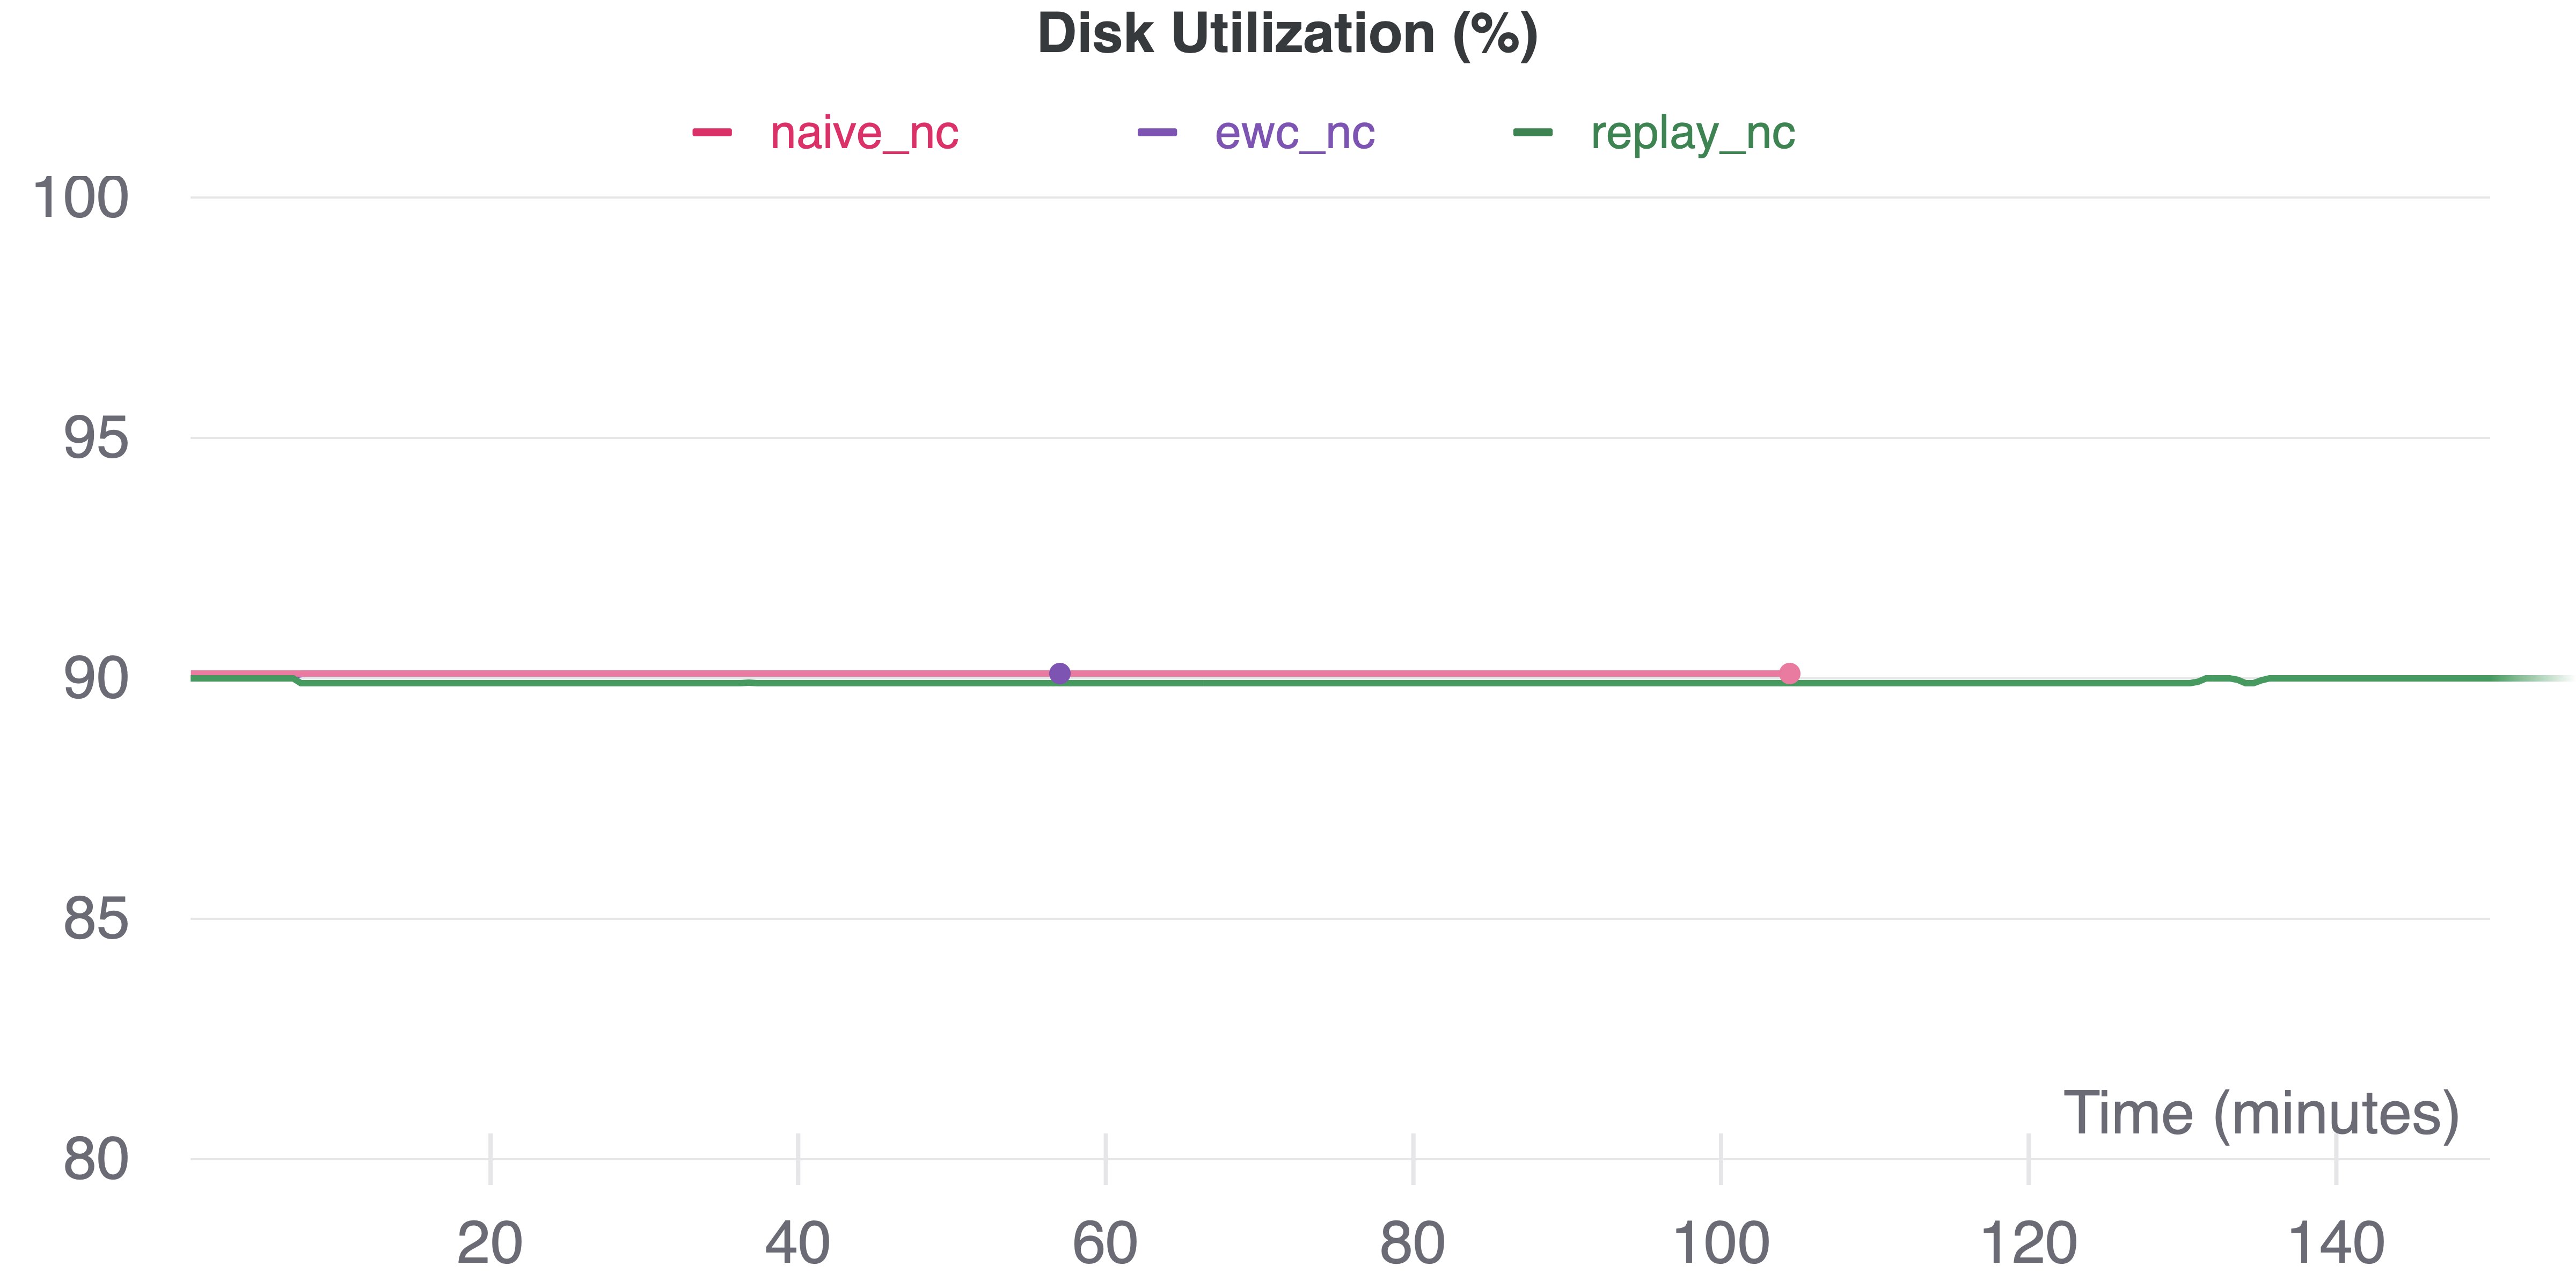
\includegraphics[width=0.60\textwidth]{overview disk utilization nc.png}
     \caption{Disk usage - multi line chart. Multi task incremental scenario}\label{Fig:106}
   
   
\end{figure}


 
\vspace{10mm}
\subsubsection{Domain incremental scenario}
In domain incremental scenario (\hyperref[Fig:106]{Figure~\ref*{Fig:107}}), there is a little difference among three algorithm. Naive strategy seems to be the one has highest impact on disk usage, until 92.5 \% , but the difference is almost imperceptible.
\begin{figure}[!h]
  
     \centering
     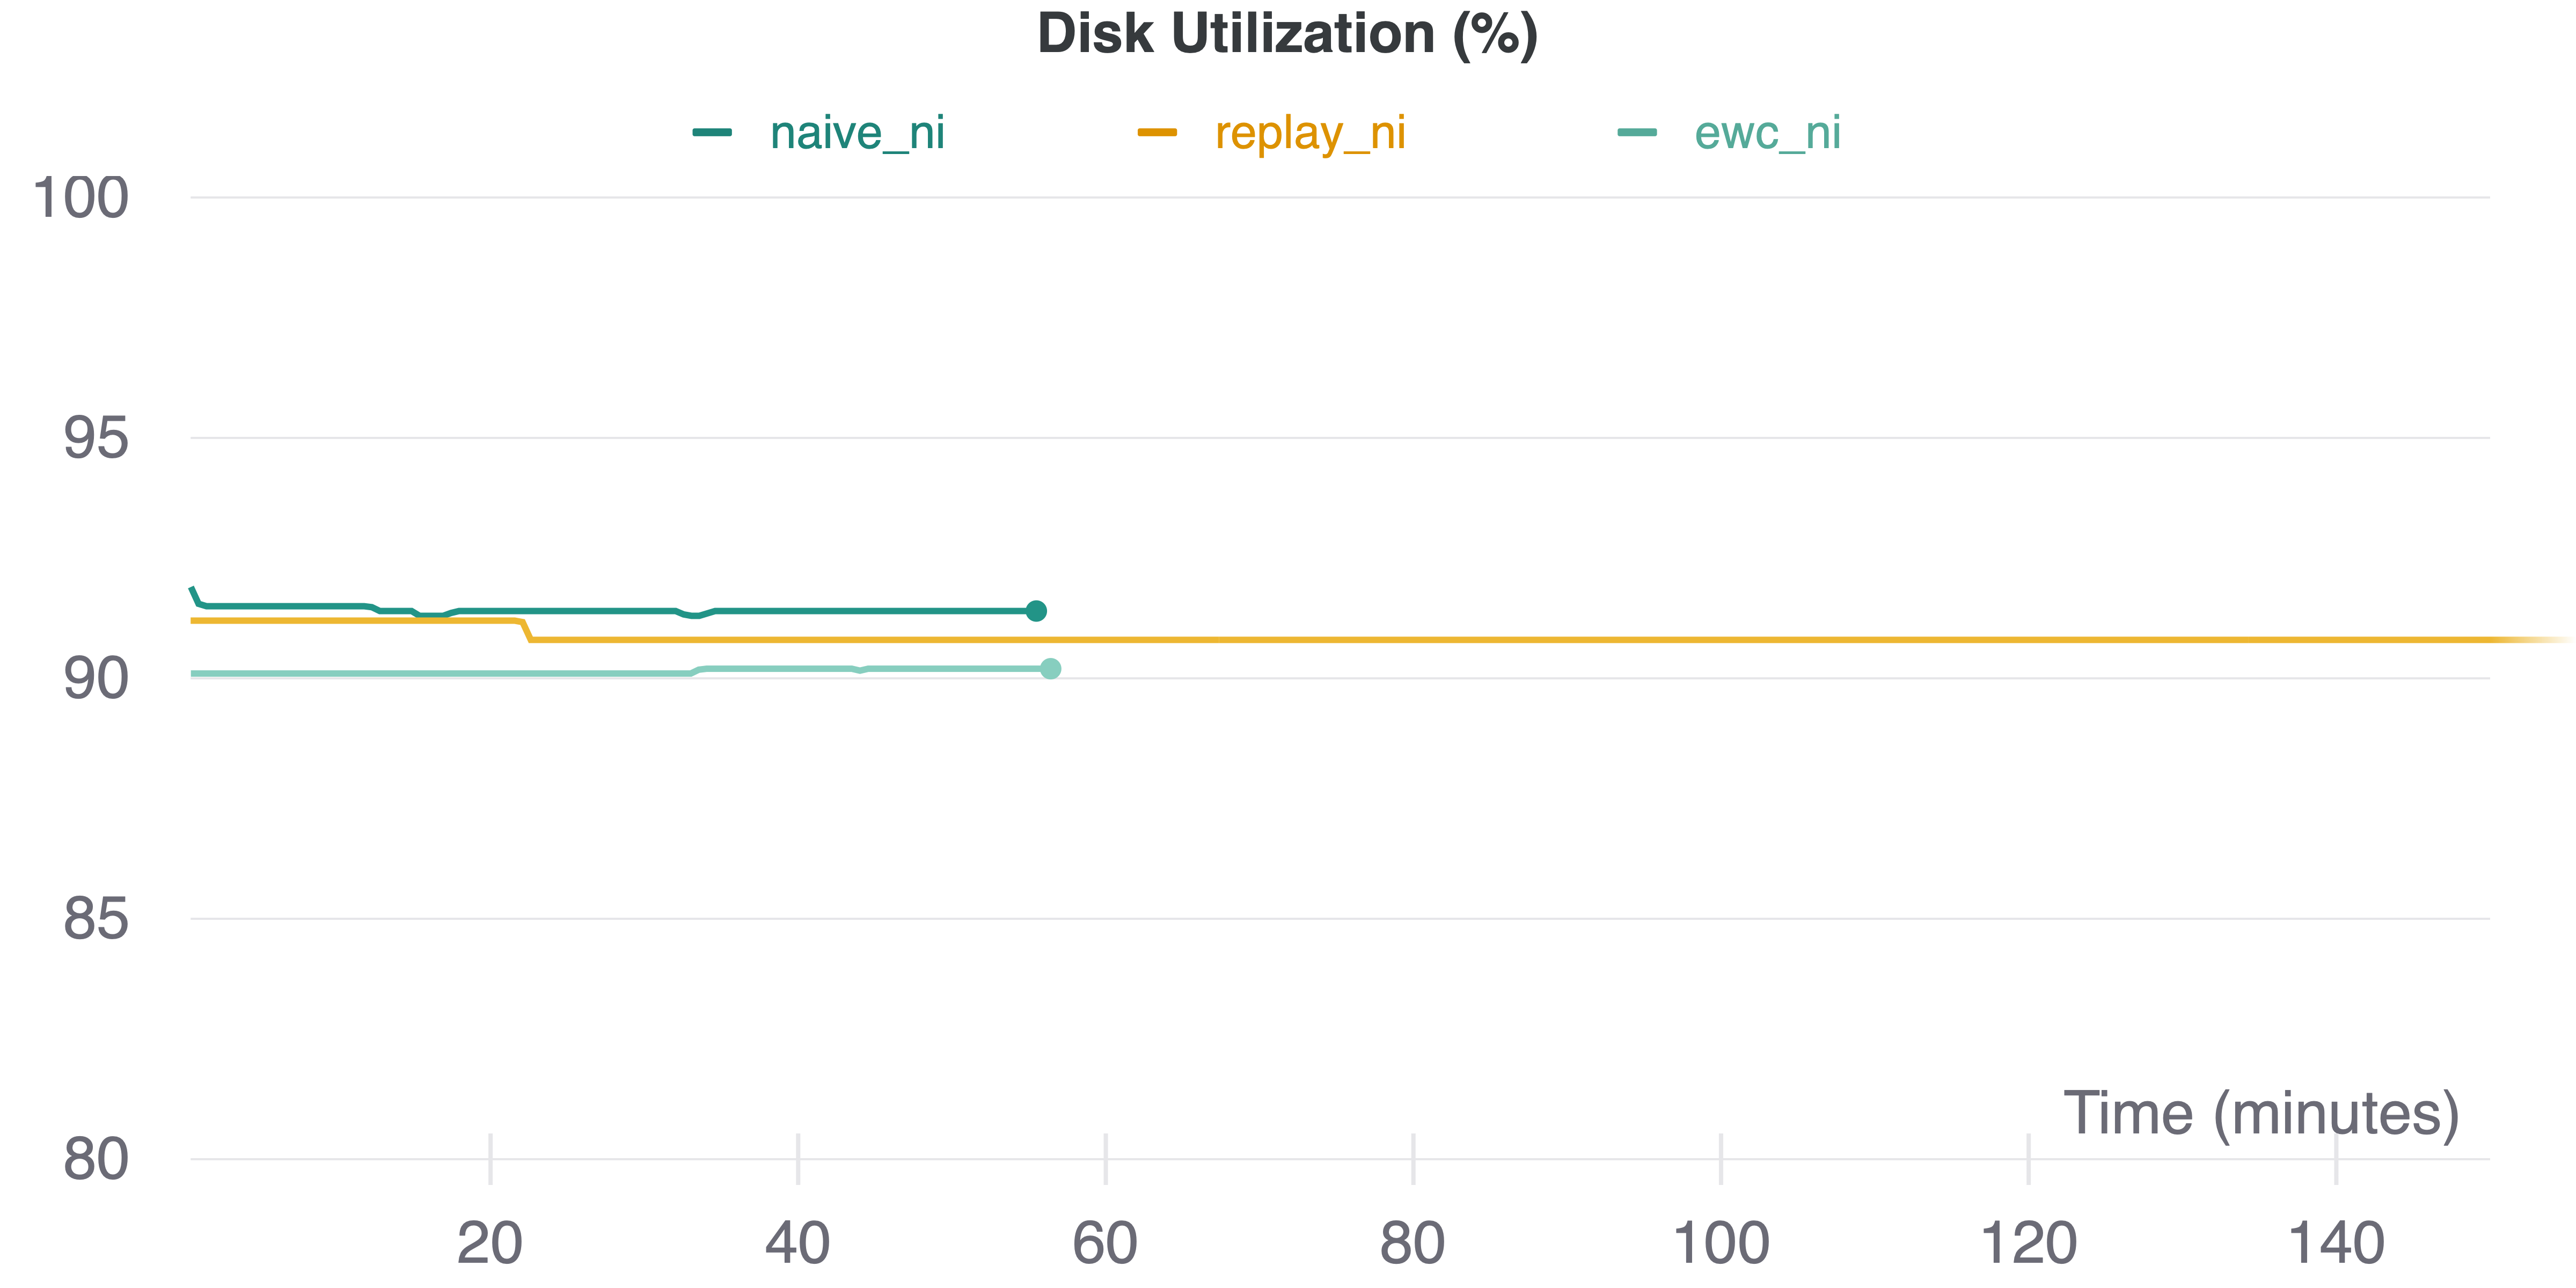
\includegraphics[width=0.60\textwidth]{overview disk utilization ni.png}
     \caption{Disk usage - multi line chart. Domain incremental scenario}\label{Fig:107}
   
   
\end{figure}




\subsection{System memory utilization usage}
System memory utilization is one of the most important system metric explored. It's fundamental because an excessive usage of RAM memory it can bring negative consequences like the interruption of the CL strategy execution or a large slowdown. In the following plots, this metric is represented by a percentage of system memory utilization in both scenarios, for all three algorithms.

\subsubsection{Multi task incremental scenario}
In this \hyperref[Fig:114]{Figure~\ref*{Fig:114}}, it is represented the evaluation of CL strategies, focusing on System Memory utilization usage metric; it is expressed by a percentage of the usage in the system. Naive and Replay strategies have an highest consuming of the RAM, reaching 65\%  of utilization. While EWC has a lower impact to system memory, it's caused by its brief duration (almost one hour).
\begin{figure}[!h]
  
     \centering
     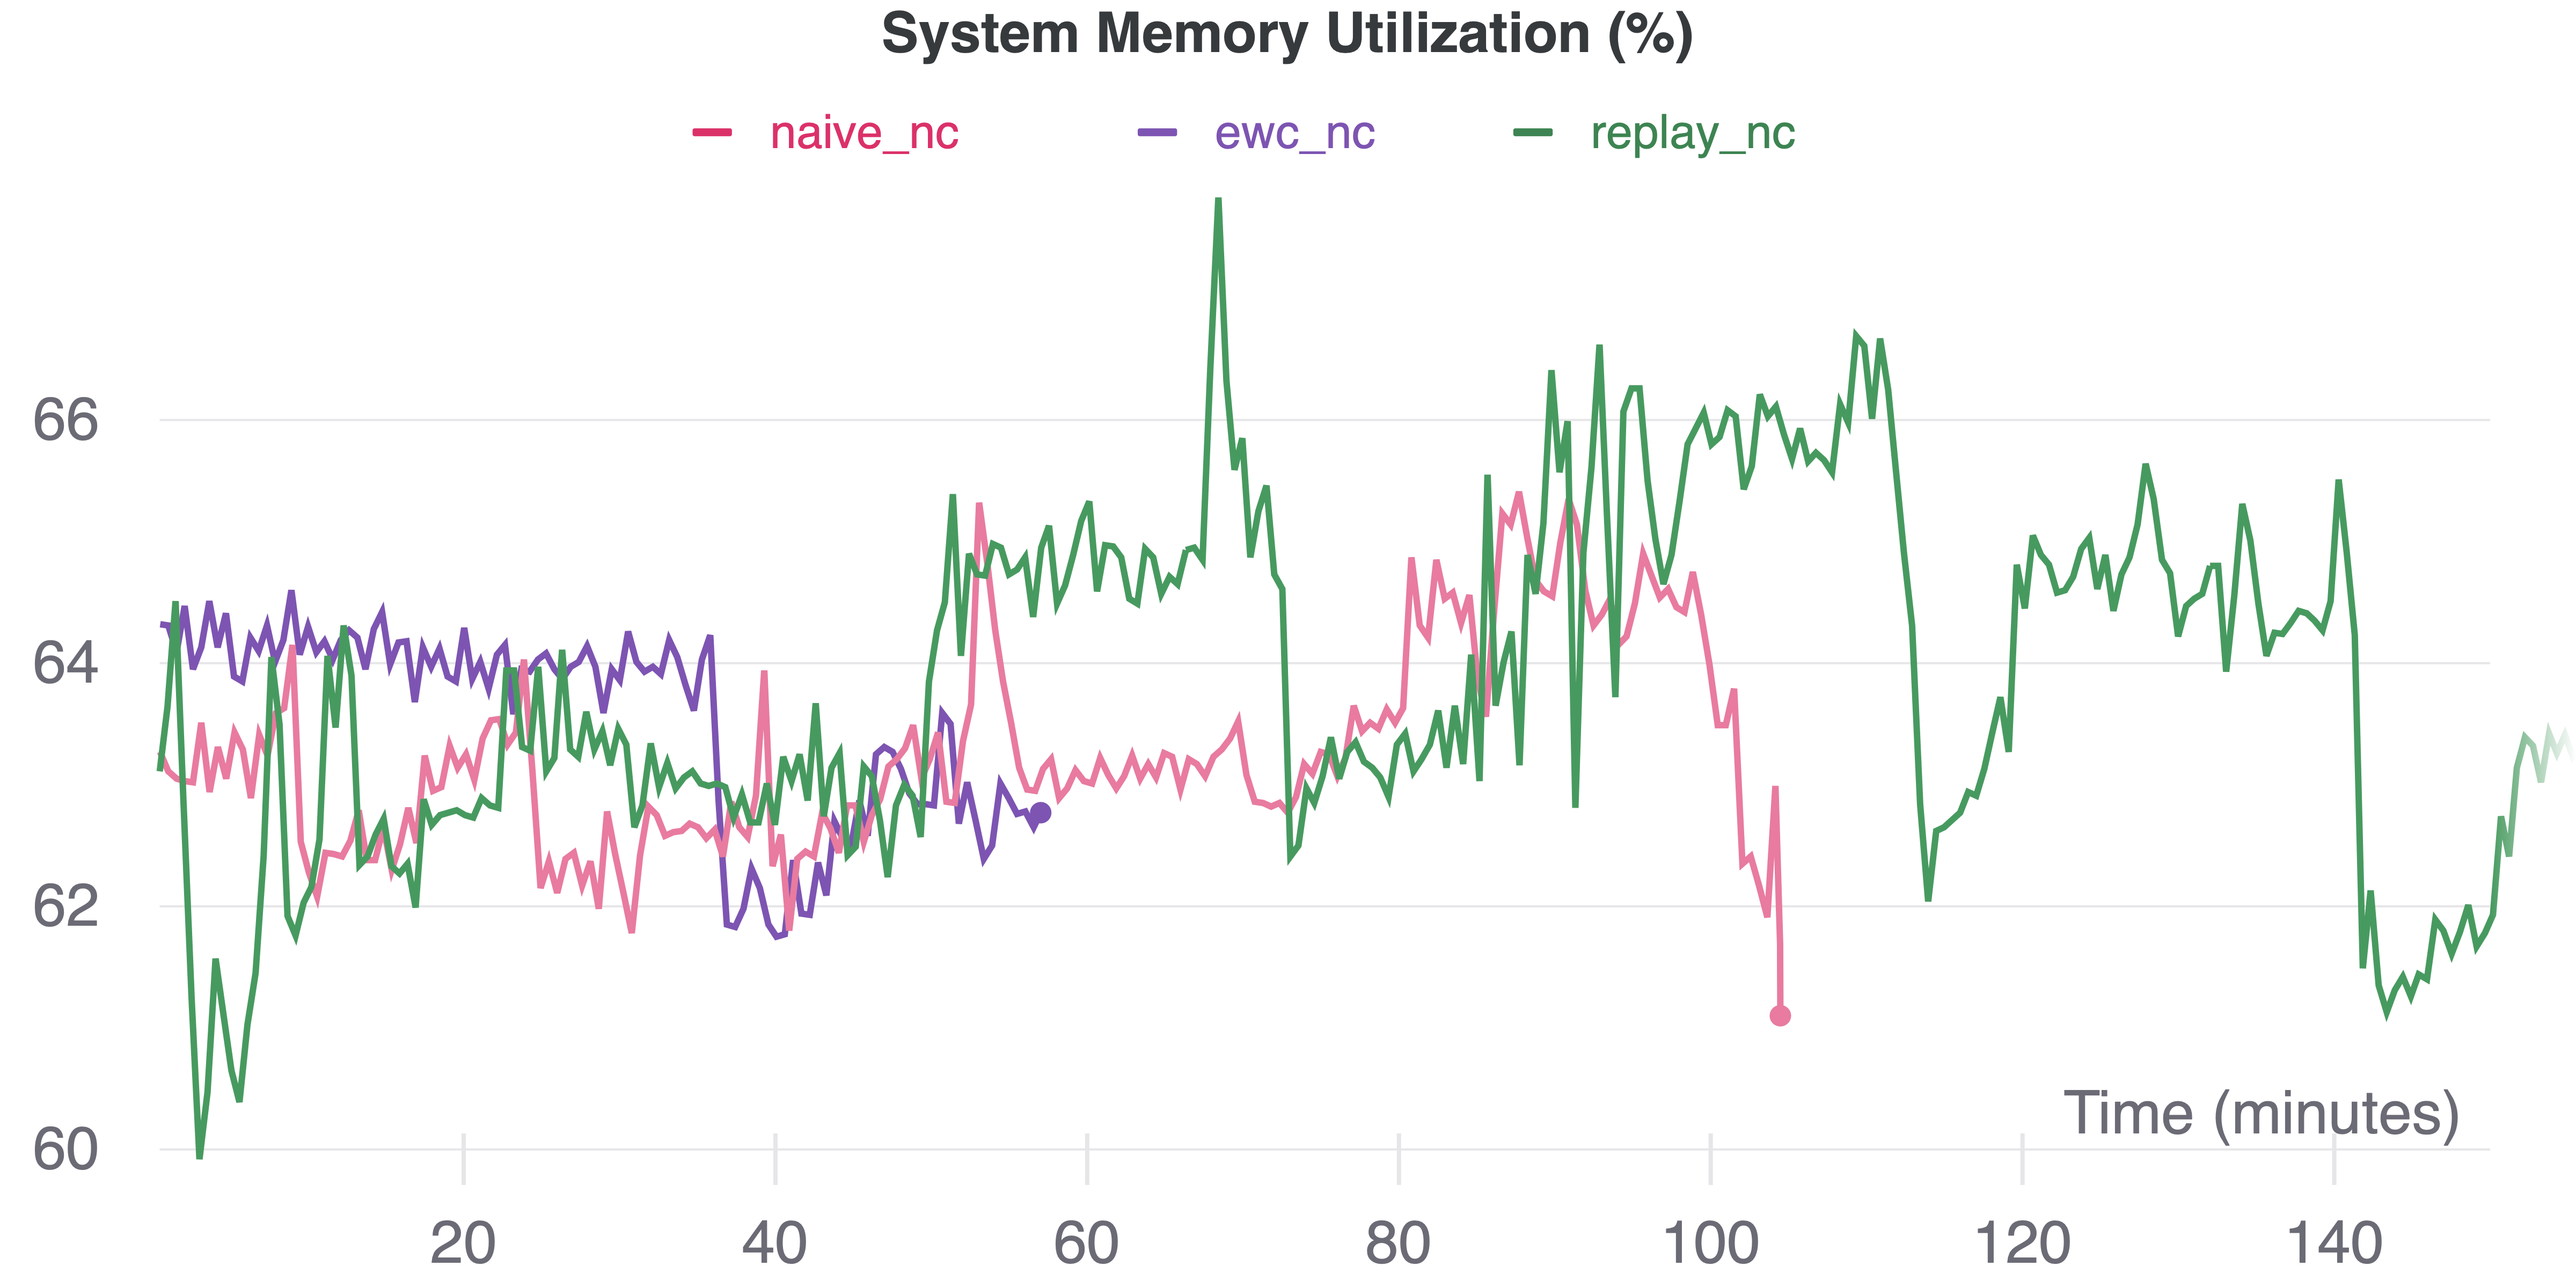
\includegraphics[width=0.60\textwidth]{overview system memory utilization nc.png}
     \caption{System memory utilization usage - multi line chart. Multi task incremental scenario}\label{Fig:114}
   
   
\end{figure}

\vspace{10mm}
\subsubsection{Domain incremental scenario}
In this second scenario, represented in \hyperref[Fig:108]{Figure~\ref*{Fig:108}}, CL strategies have different behavior. Replay has a linear  trend with an average equal to 62\%; Naive has the biggest effort on this metric, it reaches peaks equal to 65\%; while EWC, as in the other scenario, has lower impact on RAM  but in this case it hasn't the shortest duration. 
\begin{figure}[!h]
  
     \centering
     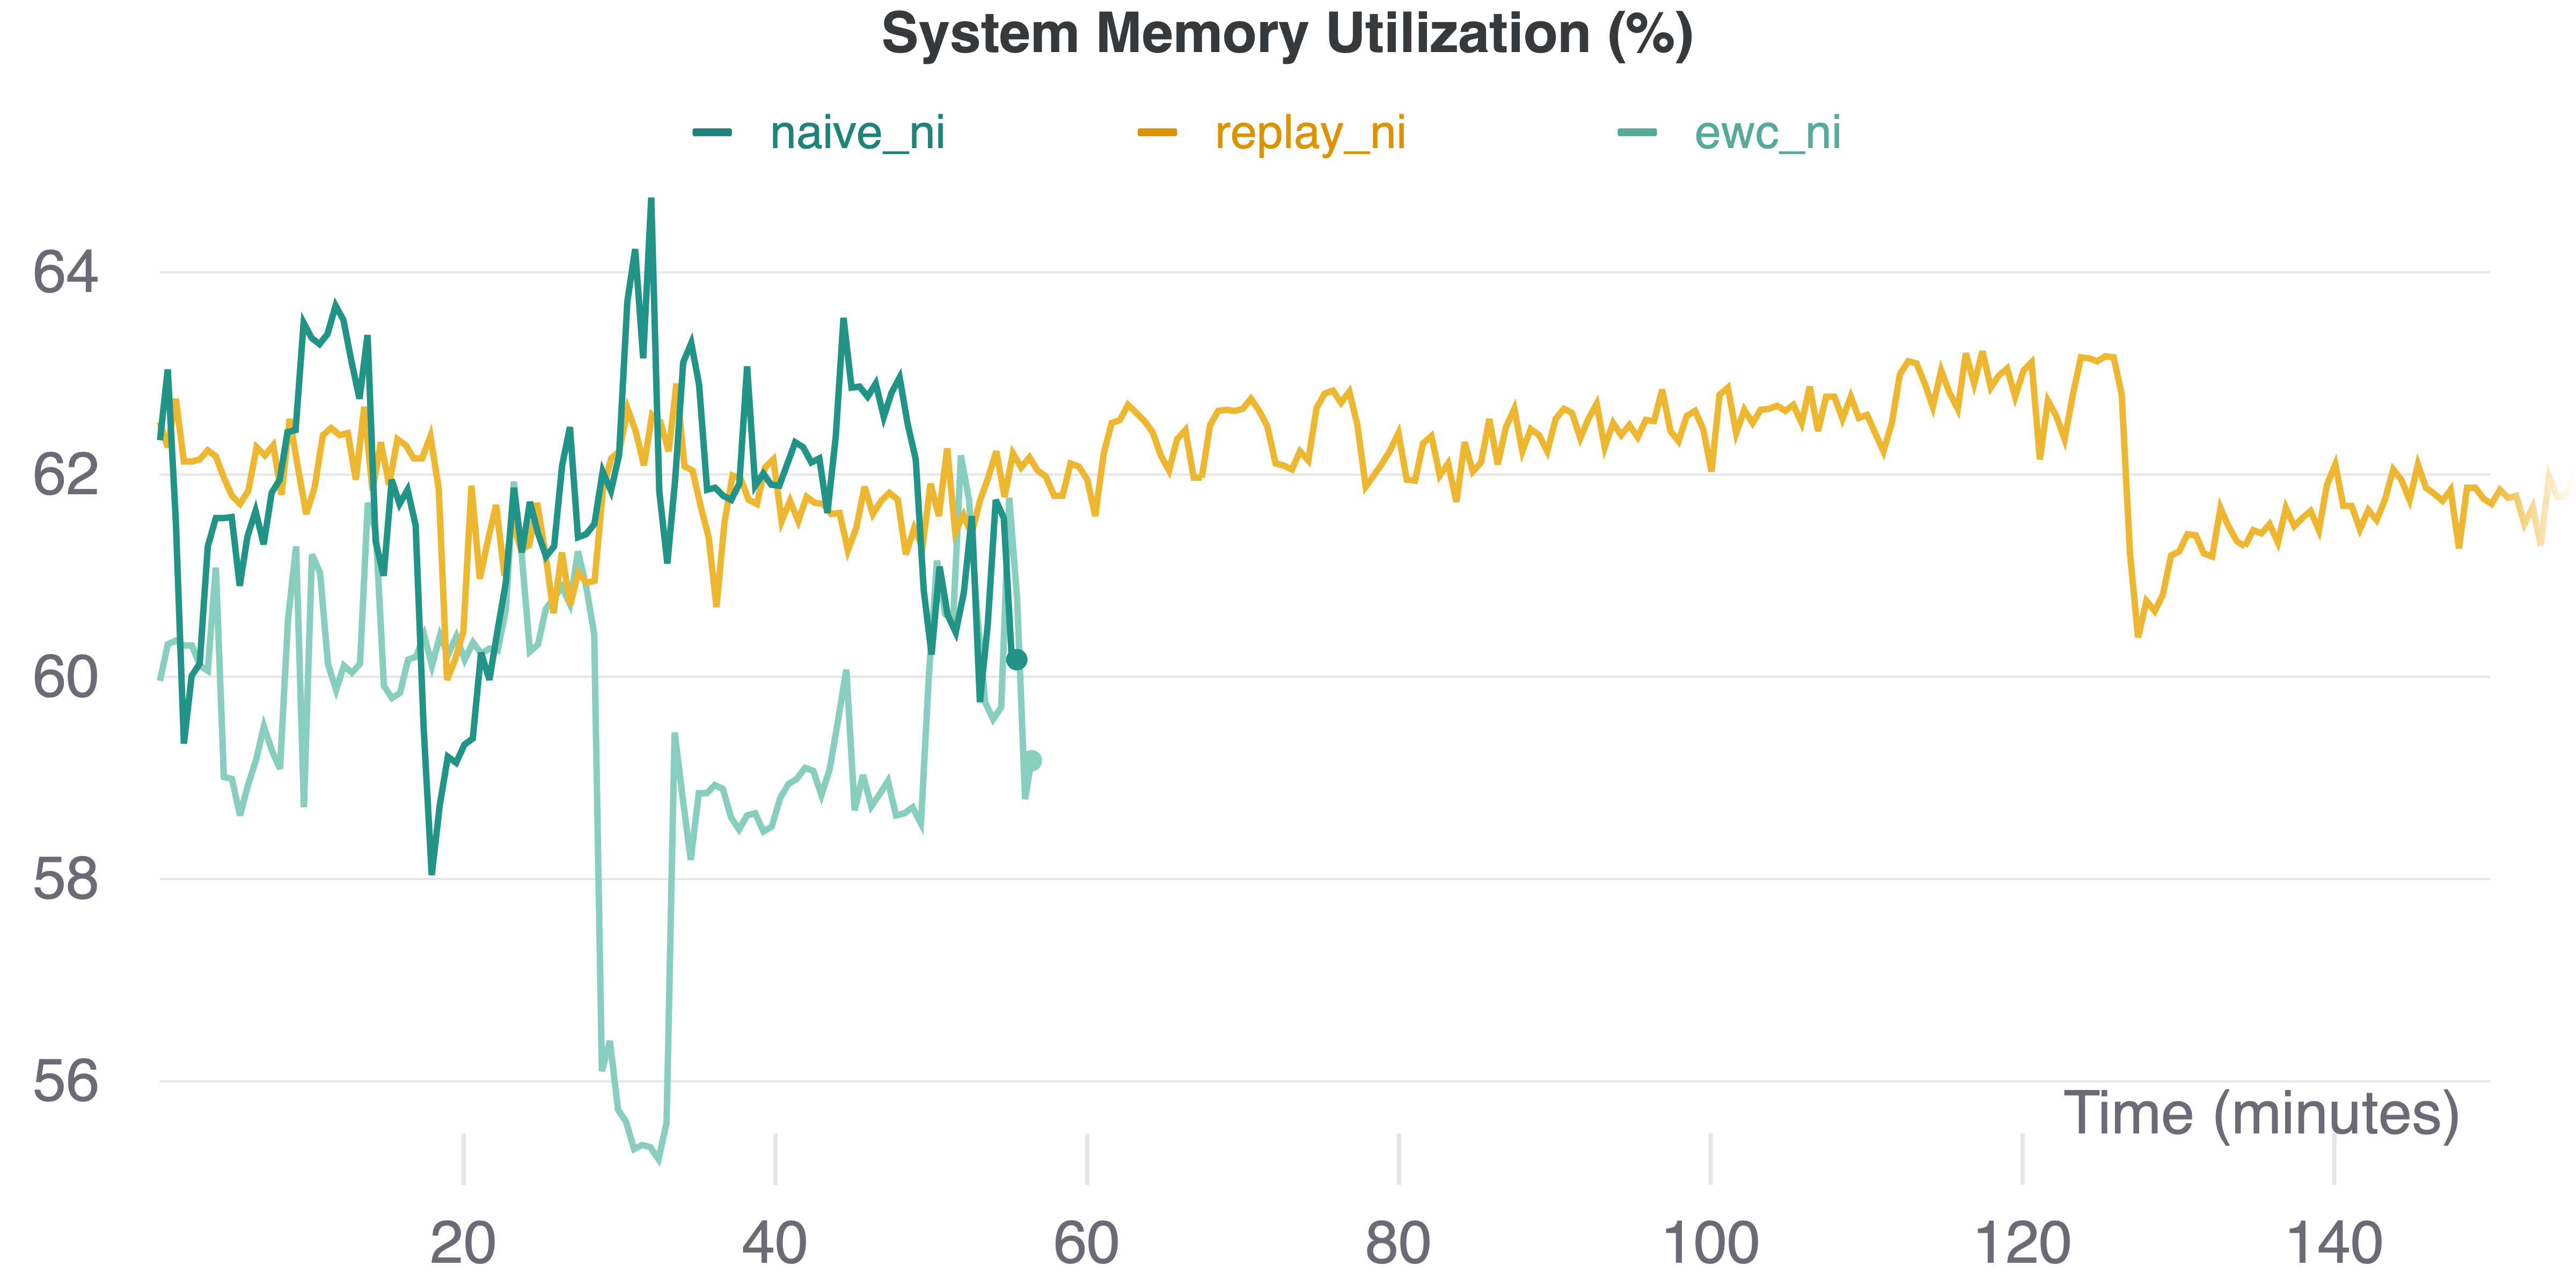
\includegraphics[width=0.60\textwidth]{overview system memory utilization ni.png}
     \caption{System memory utilization usage - multi line chart. Domain incremental scenario}\label{Fig:108}
   
   
\end{figure}
    

\subsection{Network traffic}
Network traffic refers to the amount of data moving across a network at a given point of time. Network data is mostly encapsulated in network packets, which provide the load in the network. Network traffic is the main component for network traffic measurement, network traffic control and simulation. The proper organization of network traffic helps in ensuring the quality of service in a given network.
For each scenario, network traffic is represented by two different point of view, using always bytes as a metric unit:
\begin{itemize}
    \item Network Traffic sent;
    \item Network Traffic received.
\end{itemize}

These following graphs (\hyperref[Fig:109]{Figure~\ref*{Fig:109}} and \hyperref[Fig:110]{Figure~\ref*{Fig:110}}) represent the behavior of the Network Traffic of the system where the CL strategy has been executed. The first one shows the output traffic and the second one shows the output traffic. For both graphs, x axis stays for the duration of the algorithm execution and the y axis represent the traffic in terms of byte.
\subsubsection{Multi task incremental scenario}
\begin{figure}[h]
   \begin{minipage}{0.48\textwidth}
     \centering
     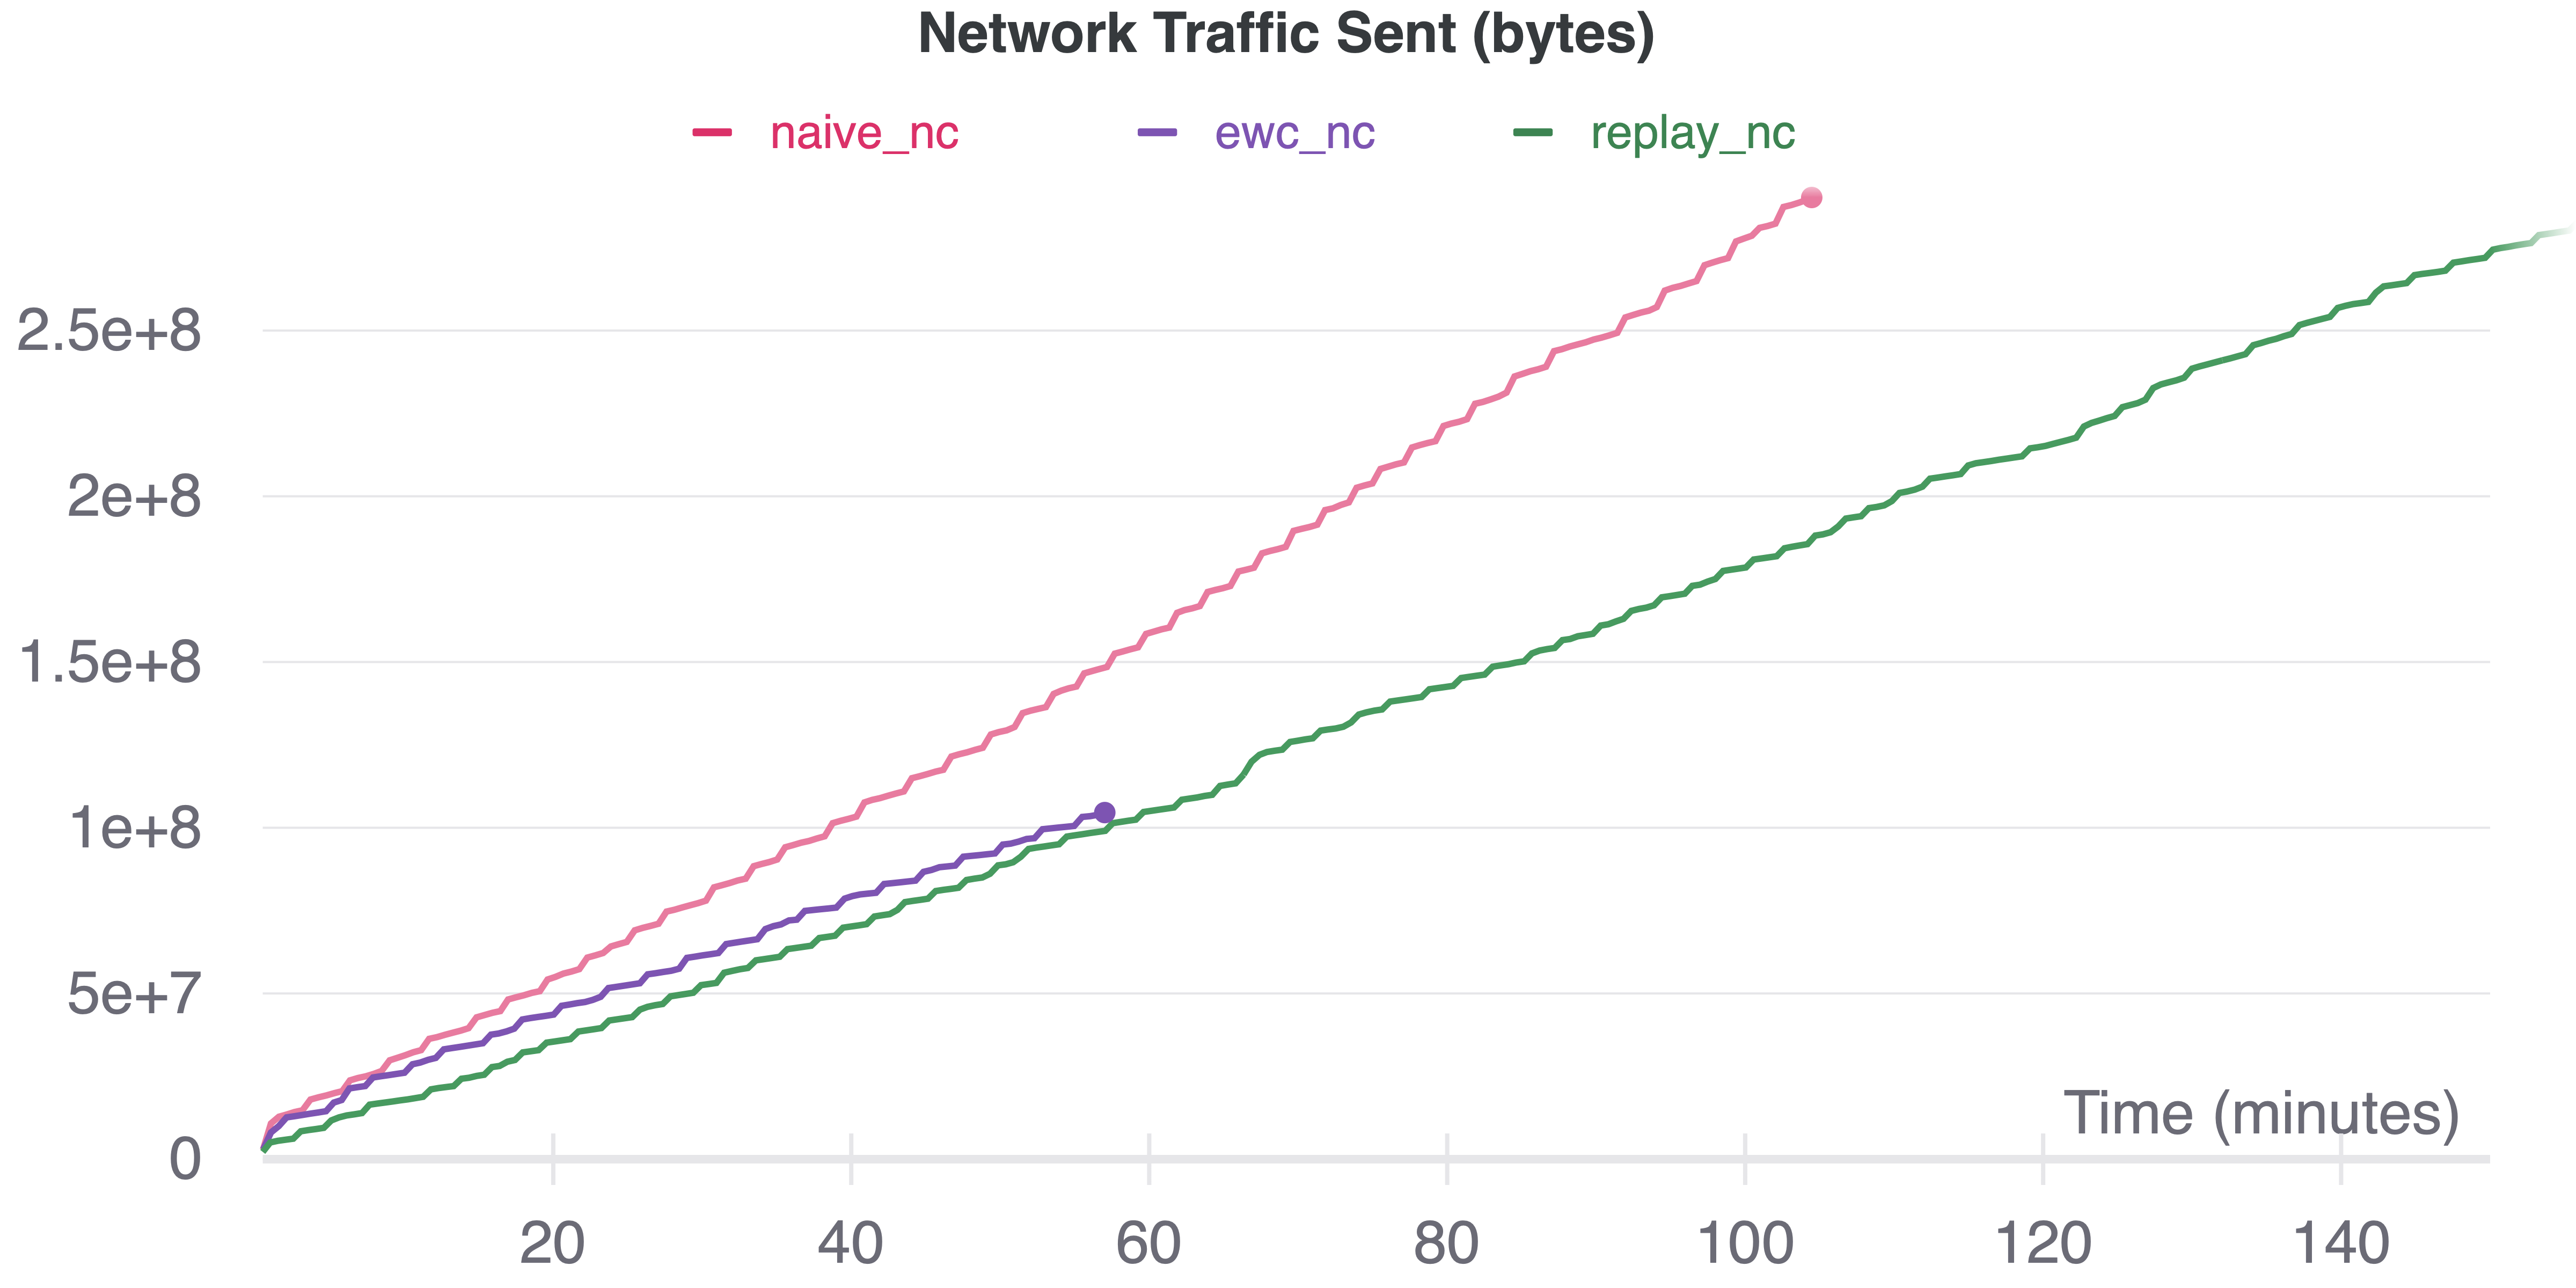
\includegraphics[width=1.1\linewidth]{overview network traffic sent nc.png}
     \caption{Network traffic sent - multi line chart. Multi task incremental scenario}\label{Fig:109}
   \end{minipage}\hfill
   \begin{minipage}{0.48\textwidth}
     \centering
     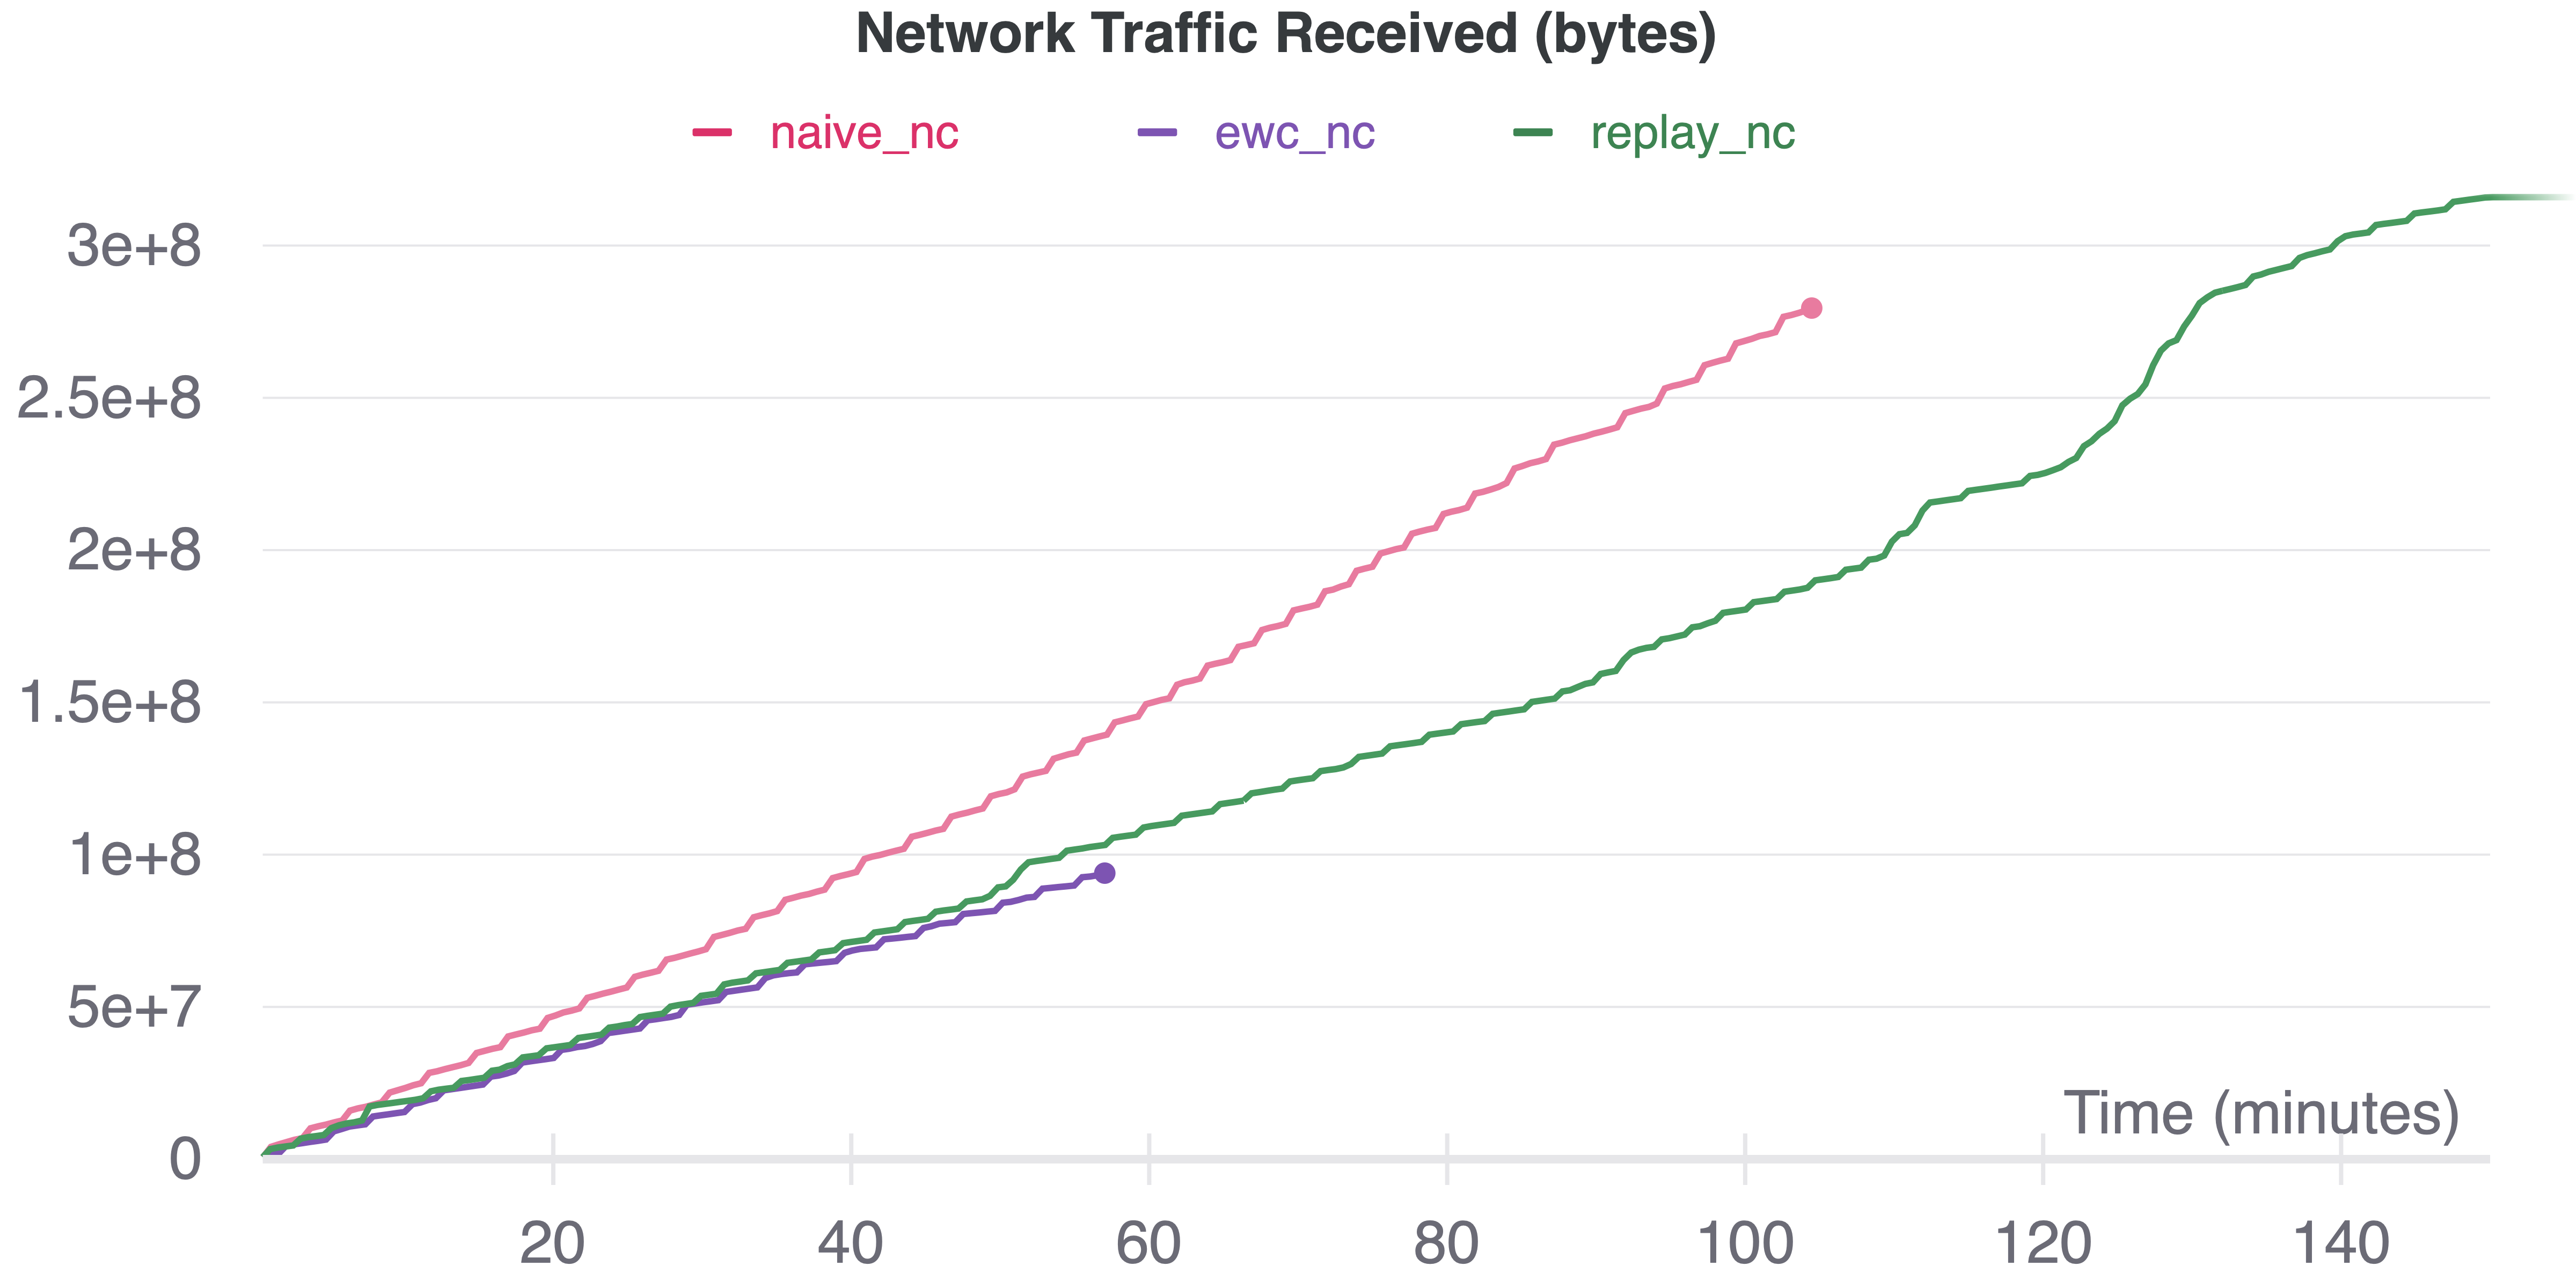
\includegraphics[width=1.1\linewidth]{overview network traffic received nc.png}
     \caption{Network traffic received - multi line chart. Multi task incremental scenario}\label{Fig:110}
   \end{minipage}
\end{figure}



For all strategies, the curve is constantly rising with the same slop; only Naive is slightly more sloping.  This one and Replay reach the same value (3e+8 bytes in traffic received and 2.5e+8 in traffic sent) but the latter one has more duration, so it means that Naive has a bigger impact from the point of view of the network traffic. The situation is the same for both cases.


\subsubsection{Domain incremental scenario}

\begin{figure}[h]
   \begin{minipage}{0.48\textwidth}
     \centering
     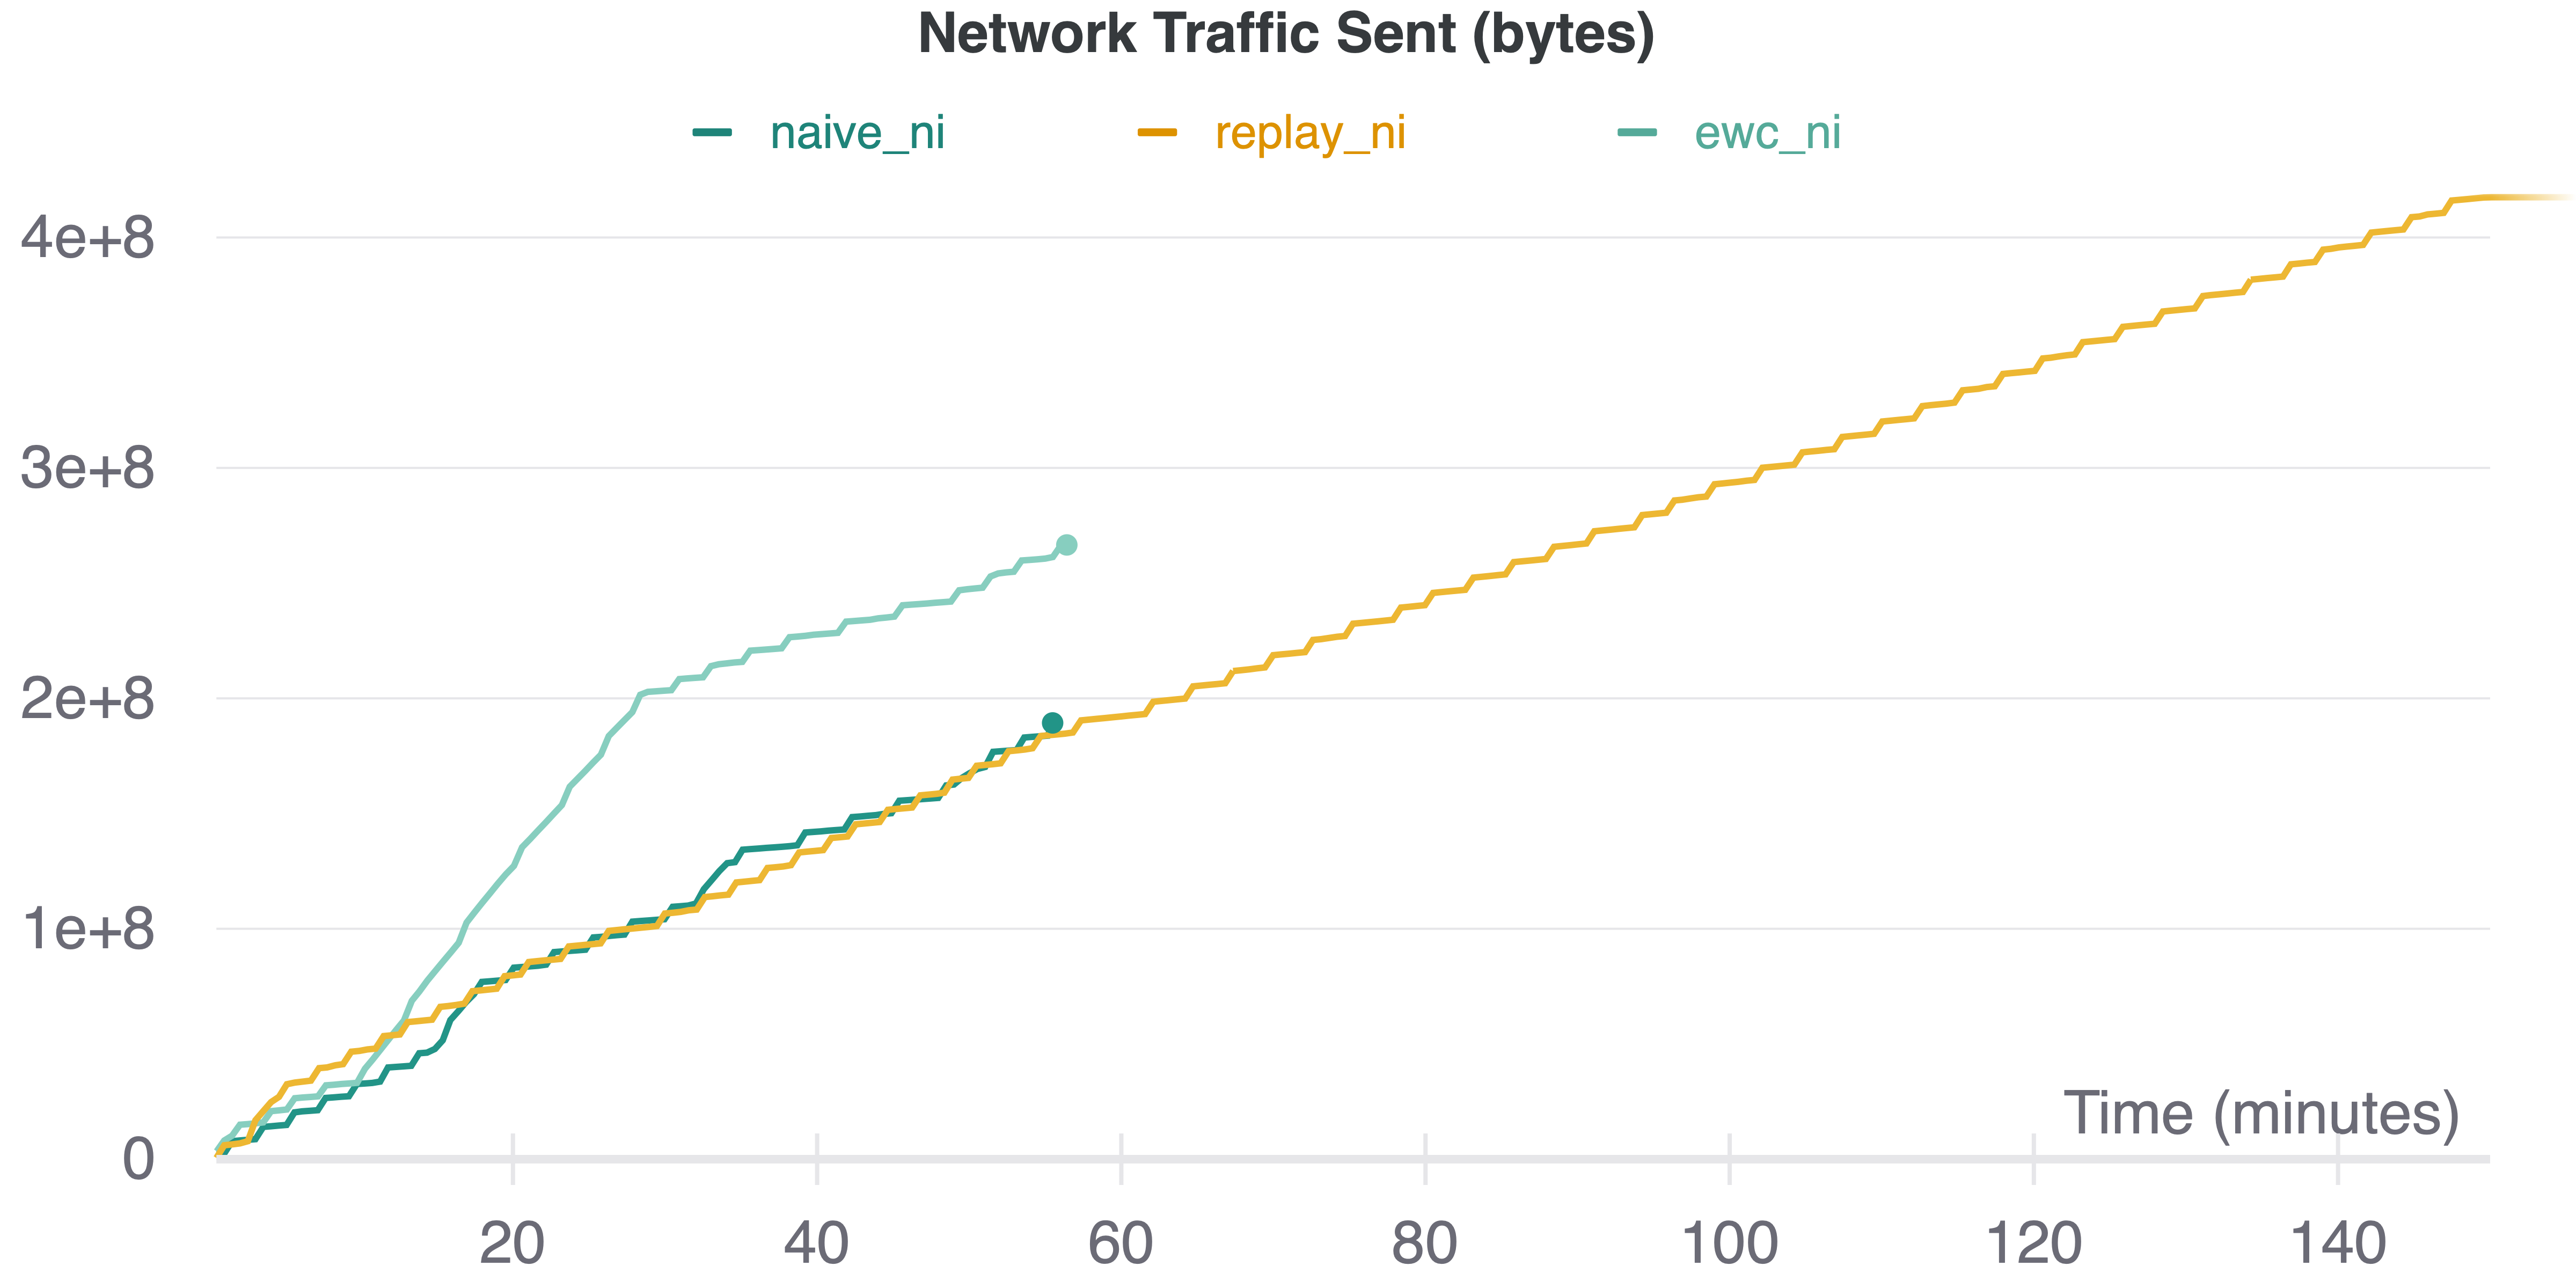
\includegraphics[width=1.1\linewidth]{overview network traffic sent ni.png}
     \caption{Network traffic sent - multi line chart. Domain incremental scenario}\label{Fig:111}
   \end{minipage}\hfill
   \begin{minipage}{0.48\textwidth}
     \centering
     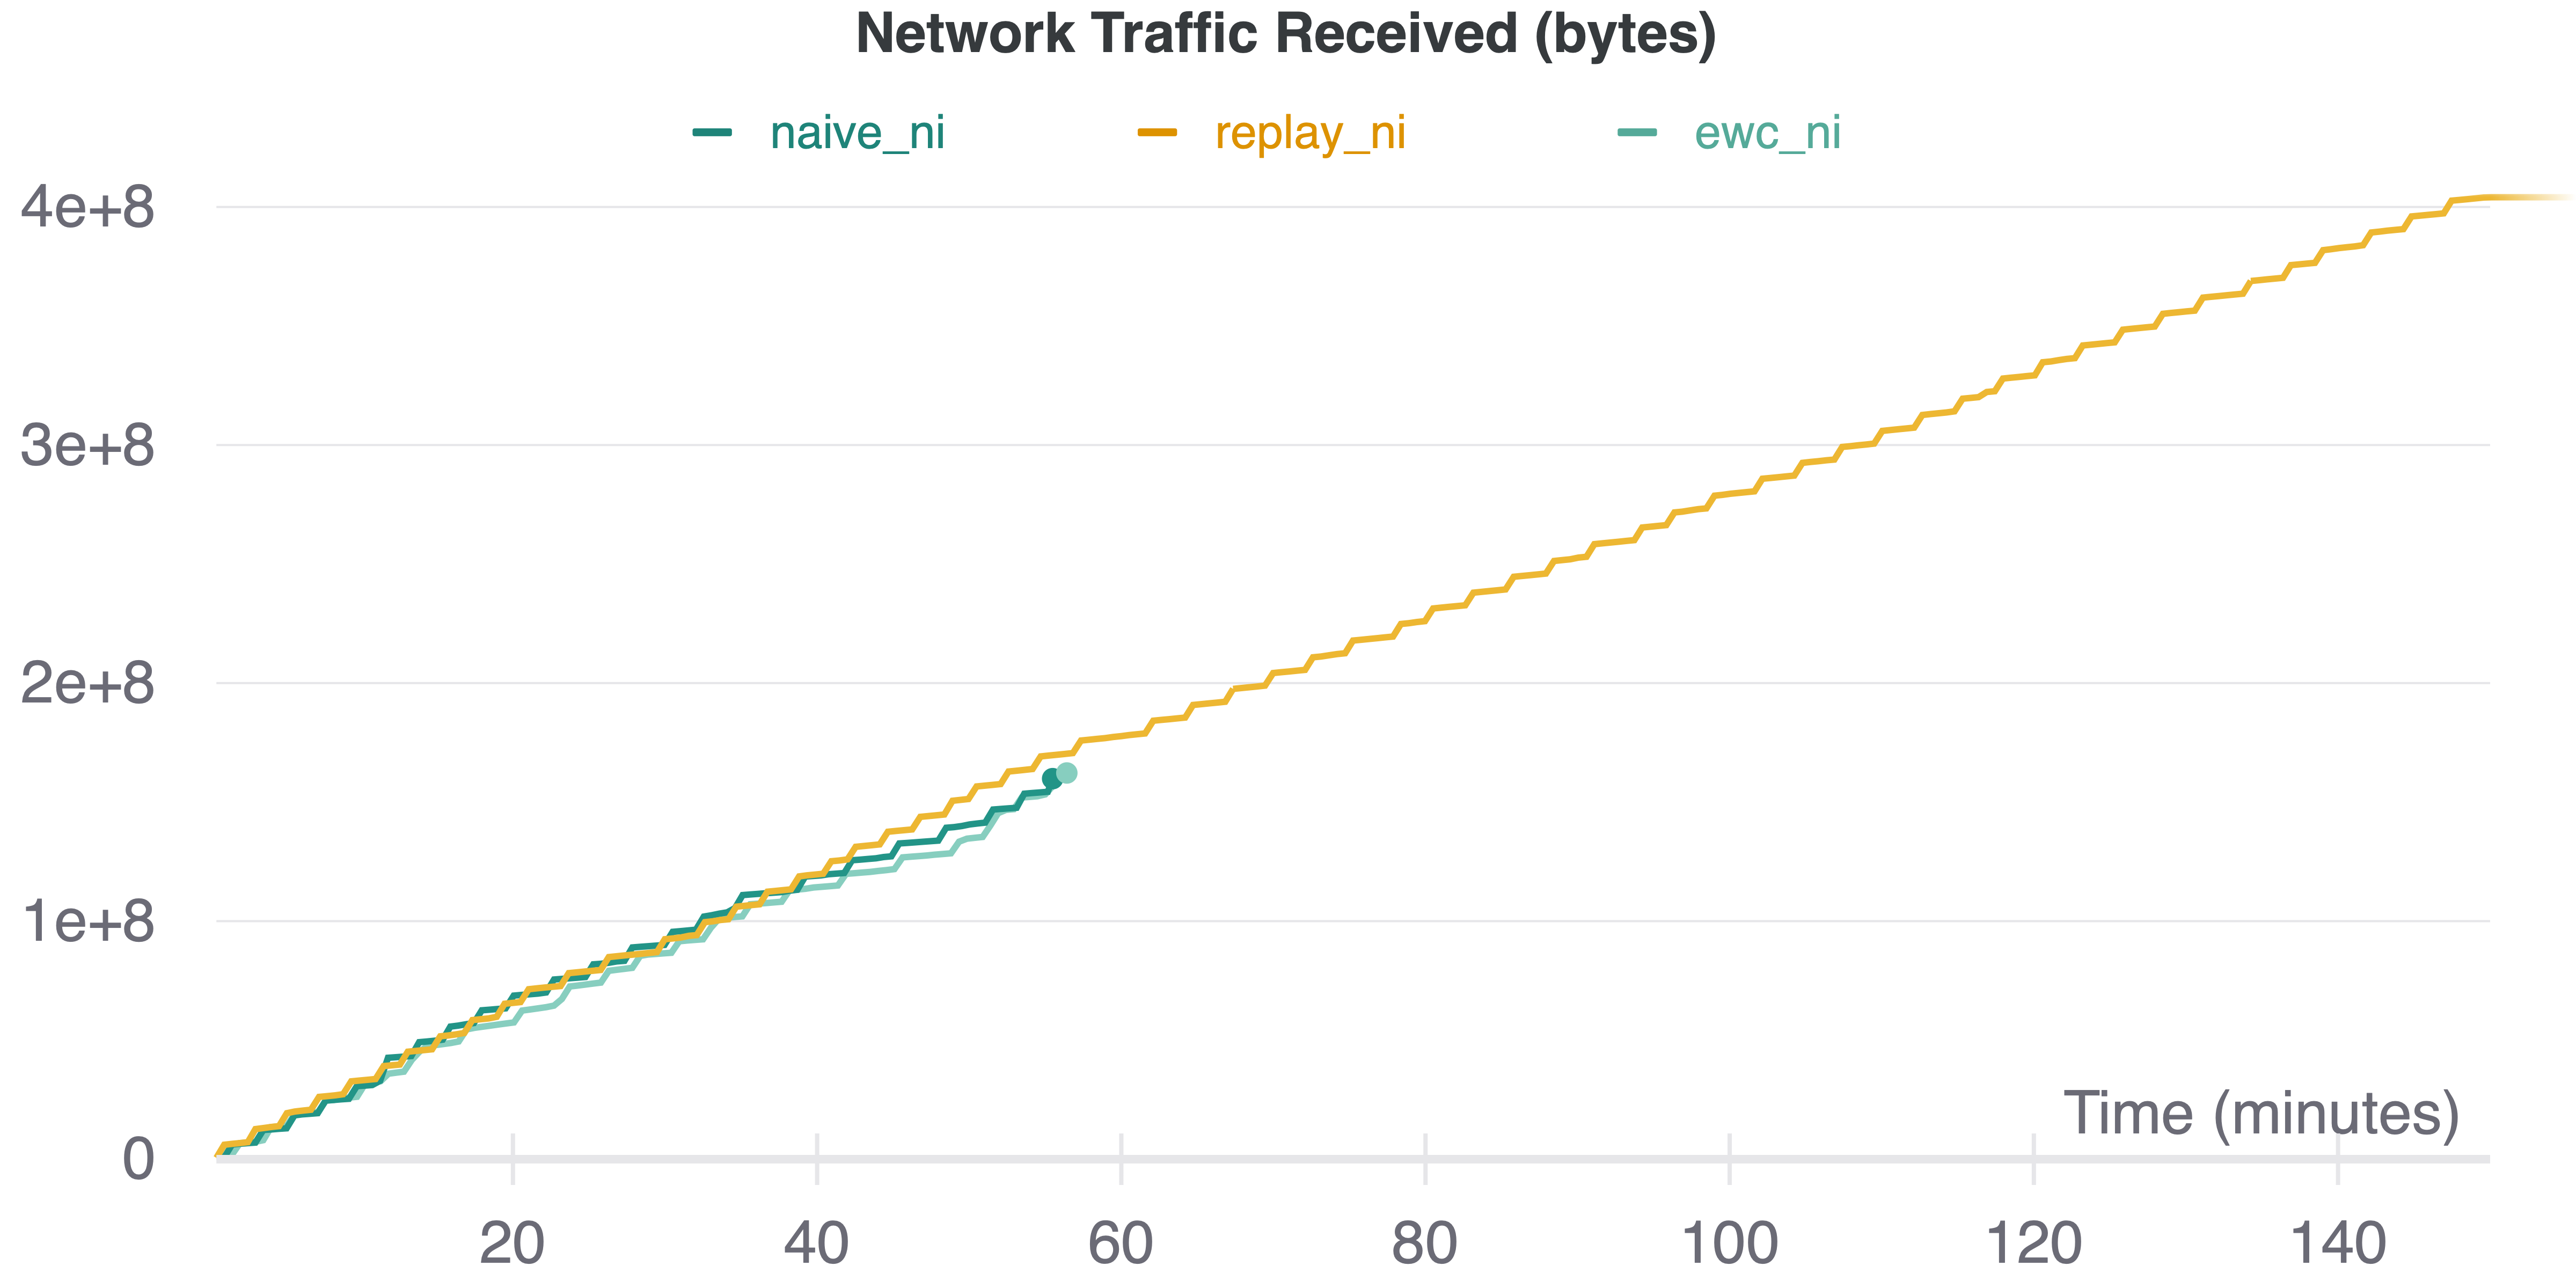
\includegraphics[width=1.1\linewidth]{overview network traffic received ni.png}
     \caption{Network traffic received - multi line chart. Domain incremental scenario}\label{Fig:112}
   \end{minipage}
\end{figure}
In Domain Incremental scenario (\hyperref[Fig:111]{Figure~\ref*{Fig:111}}), the situation is a bit different among strategies. In second graph  (\hyperref[Fig:112]{Figure~\ref*{Fig:112}}), the network traffic received is the same for each algorithm while the situation in network traffic sent is different: EWC has more impact about the traffic sent in few time. If we consider all execution time, Replay consumes more bytes because this strategy needs more time for its execution.


\part{Conclusions}


\chapter{Conclusions \& Future works}

\section{Conclusions}
The intent of this work was to provide a number of original contributions to the early development of continual learning research in the context of deep architectures for AI. The objective was to propose such contributions within a general approach to continual learning taking into account different, little experienced so far application field. The focusing was on evaluating of different Continual learning strategies on new benchmark based on audio dataset for the event sound classification.


An overview of the field of Continual Learning has been covered, describing typical architectures such as the several explored scenarios and all main concepts. Some CL strategies have been detailed, as well.
\newline \newline
In this thesis we presented a novel library to support the developments in the field of Continual Learning, extending and adapting work from the Continual Learning community on audio classification; it's named Avalanche.
This library has been used to develop and test all features of this thesis work, from the creation of a new benchmark based on audio dataset to an evaluation of CL strategies on this newly benchmark. Avalanche has proved to be of fundamental importance in the realization of this work; it allows to show vastly some complete and robust results that are reported in previous chapter.
\newline \newline
Summarizing, the key contributions of this work are:
\begin{itemize}
    \item Understanding the possible development of a new Continual Learning benchmark based on audio dataset for the sound classification, analyzing all features about audio classification. The usage of this framework can be very useful in the context of audio data, especially  by the length of every item and the dependence of currently explored data from the previously;
    \item The development two type of benchmark based on two different CL scenario: Multi task incremental and Domain Incremental that have been considered  most suitable for the audio classification.  Both benchmarks are created by a basic audio dataset (\textit{ESC-50}) that allow us to have a good starting point for this new exploration.
    All implementation has been done through Avalanche, as new integrated section of this library along with other several benchmark (based on image data) that itself offers.
    \item The definition of these benchmarks allow us to evaluate different CL scenario in a new scope of the audio classification. This evaluation has been done through several available CL metrics that have been considered suitable for this purpose. All evaluations for each metric have been performed by Avalanche library, using different provided methods. From this phase we got some interesting results and related considerations of this experiment.
\end{itemize}

At the end of the thesis work, it's possible to get some considerations about final results that have been obtained by the graphs of different CL metrics and then give some further points for possible future works that will be introduced in next section.
\newline \newline
For some metrics, such as Accuracy and Loss, the results are not very good in terms of value; but if we take in consideration that they are obtained by using CL strategies (Avalanche) created for image classification, they can be considered as a relevant starting point to create or improve existing algorithm also for this scope.
Moreover it's evident that if we compare considered scenarios, multi task incremental is the best in terms of accuracy and loss, obtaining good values, while considering forgetting and Backward Transfer (BWT) metrics the situation is completely different and  Domain Incremental is better than other one because there is no forgetting and consequently BWT assumes more grateful scores.
\newline \newline
Regarding CL strategies adopted, it's evident from the results discussed in previous chapter that the best algorithm is Replay; in both scenarios it seems to get the best scores for all point of view of performances. 
Replay is also the strategy that needs more time to complete its execution for both phase (training and evaluation) and it requires more effort of the system where algorithm is executed. Considering all different system metrics (RAM/CPU/Disk usage and network traffic) the performance of the system during all strategies is almost the same; the duration of them is quite different and it change remarkably the performance over the machine.

From the same point of view, it's evident also that Elastic Weight Consolidation (EWC) works badly in this context; in both scenarios the performance is not good so this CL algorithm  can be excluded in working experiments for the Event Sound Classification.
\newline \newline
By concluding these final considerations, a big contributions for this thesis has been given by Avalanche. With this library, it was possible implement and build new Continual Learning benchmarks and test all strategies on them. All work done can be considered as an integration of this library; nowadays it offers only benchmark suitable for the image classification. In next section, some possible future works (also in this context) are introduced, starting from this thesis work.

\section{Future works}
The results of the experiments in this thesis point to several directions and options for further experimentation with Continual Learning architecture.
Having the goal of providing a shared and collaborative open-source codebase for all CL applications, Avalanche is always looking to add and refine functionalities as the space for improvements in such a framework is large, even more focusing on field that haven't explored yet.
As previously described, the implementation of the benchmark and related tests can be included as new branch of this library.
\newline \newline
Further implementations on Continual Learning can be done starting from this work, regardless of using Avalanche.  From new created benchmarks, it would be interesting to explore more strategies over them, exploring all metrics and related results, trying also to create or change current Avalanche strategies, adopting them for specific purpose of the audio classification. Focusing on the Replay strategy and avoiding exploring the EWC can be a good starting point for deepening the work among all possible CL algorithms.
Moreover, it's possible to explore different feature of audio data, beyond Environment Sound Classification, building new benchmarks from new dataset suitable for other specific tasks.
\newline \newline
Nowadays Continual Learning is a very innovative framework of the Deep Learning, but it has still many features to explore better, mostly regarding several possible application fields, such us the audio. Starting from Avalanche library, multiple developments can be done about that; it's a outstanding library with large margins for improvement that can lead big evolution in AI literature, focusing on audio classification in Continual Learning field, that will be surely the leading actor in Deep Learning for next years.
\newline \newline






\backmatter
\phantomsection
\begin{thebibliography}{17}

\bibitem{Hinton-2006}
Hinton, G. E., Osindero, S., and Teh, Y.-W. (2006). \textit{A fast learning algorithm for deep belief nets. Neural Comput.}

\bibitem{deep-learning}
Yann LeCun, Yoshua Bengio & Geoffrey Hinton (2015). \textit{Deep Learning}

\bibitem{neural-network}
Jürgen Schmidhuber.  \textit{Deep learning in neural networks: An overview. Neural networks.}

\bibitem{act_function}
Shivam Bhardwaj (2021).  \textit{Neural Networks and Activation Function}.

\bibitem{ring}
Mark Bishop Ring. (1994)\textit{Continual learning in reinforcement environments.}

\bibitem{cat_forgetting}
Robert M. French. \textit{Catastrophic forgetting in connectionist networks. Trends in Cognitive Sciences.}

\bibitem{goodfellow}
Goodfellow, I., Bengio, Y., and Courville, A. (2016).  \textit{Deep Learning, volume 1.}

\bibitem{lecun}
LeCun, Y., Bengio, Y., and Hinton, G. (2015)  \textit{Deep learning. Nature.} 



\bibitem{hoiem}
Li, Z. and Hoiem, D. (2016).  \textit{Learning without forgetting. In 14th European Conference on Computer Vision (ECCV 2016), volume 9908 LNCS.}

\bibitem{Kirkpatrick}
Kirkpatrick, J., Pascanu, R., Rabinowitz, N., Veness, J., Desjardins, G., Rusu, A. A., Milan, K., Quan, J., Ramalho, T., Grabska-barwinska, A., Hassabis, D., Clopath, C., Kumaran, D., and Hadsell, R. (2017). \textit{Overcoming catastrophic forgetting in neural networks.}

\bibitem{zhang}
H. Zhang, I. McLoughlin, and Y. Song. (2015). \textit{Robust sound event recognition using convolutional neural networks.} 

\bibitem{valenti}
 M. Valenti, A. Diment, G. Parascandolo, S. Squartini, and T. Virtanen (2016). \textit{Dcase 2016 acoustic scene classification using convolutional neural networks.} 

\bibitem{gemmeke}
J. F Gemmeke, D. P. W. Ellis, D. Freedman, A. Jansen, W. Lawrence, R. C. Moore, M. Plakal, and M. Ritter (2017). \textit{Audio set: An ontology and human-labeled dataset for audio events.} 
 
 \bibitem{bello}
 J. P. Bello, C. Silva, O. Nov, R. L. Dubois, A. Arora, J. Sala- mon, C. Mydlarz, and H. Doraiswamy (2019). \textit{Sonyc: A system for monitoring, analyzing, and mitigating urban noise pollution.} 
 
 \bibitem{salamon}
 J. Salamon, J. P. Bello, A. Farnsworth, M. Robbins, S. Keen, H. Klinck, and S. Kelling (2016). \textit{Towards the automatic classifica- tion of avian flight calls for bioacoustic monitoring.} 
 
  \bibitem{drossos}
  K. Drossos, S. Lipping, and T. Virtanen (2020). \textit{Clotho: an audio captioning dataset.} 

\bibitem{sprechamn}
 P. Sprechmann, S. Jayakumar, J. Rae, A. Pritzel, A. P. Badia, B. Uria, O. Vinyals, D. Hass- abis, R. Pascanu, and C. Blundell (2018). \textit{Memory-based parameter adaptation,} In International Conference on Learning Representations. 

 \bibitem{french}
 R. M. French. (1999). \textit{Catastrophic forgetting in connectionist networks. Trends in Cognitive Sciences.} 
 
 
  \bibitem{gepperth}
A. Gepperth and B. Hamme (2016). \textit{Incremental learning algorithms and applications.} 
 
   \bibitem{chen-2018}
Chen, Z. and Liu, B. (2018). \textit{Lifelong Machine Learning. Morgan & Claypool Publishers.} 


\bibitem{turing}
Turing, A. M. (1950). \textit{Computing Machinery and Intelligence.} 

\bibitem{weng}
Weng, J. (2001). \textit{ARTIFICIAL INTELLIGENCE: Autonomous Mental Development by Robots and Animals.} 

\bibitem{thrun-mitchell}
Thrun, S. and Mitchell, T. M. (1995). \textit{Lifelong Robot Learning. The biology and technology of intelligent autonomous agents.} 

\bibitem{thrun}
Thrun, S. (1996). \textit{Explanation-Based Neural Network Learning: A Lifelong Learning Approach.} 

\bibitem{carloson}
Carlson, A., Betteridge, J., Kisiel, B., Settles, B., Hruschka Jr, E. R., and Mitchell, T. M. (2010). \textit{Toward an architecture for never-ending language learning.} 

 \bibitem{mithcell-thrun}
Mitchell, T. M. and Thrun, S. B. (1993).  \textit{Lifelong robot learning.} 


\bibitem{parisi}
Parisi, G. I., Kemker, R., Part, J. L., Kanan, C., and Wermter, S. (2018). \textit{ Continual Lifelong Learning with Neural Networks.} 
 
\bibitem{creaye}
Craye, C., Lesort, T., Filliat, D., and Goudou, J.-F. (2018). \textit{Exploring to learn visual saliency.}  
 
\bibitem{michalski}
Michalski, R. S., Carbonell, J. G., and Mitchell, T. M. (2013). \textit{Machine learning: An artificial intelligence approach.}   
  
\bibitem{ring-2005}
Ring, M. B. (2005). \textit{Toward a Formal Framework for Continual Learning.}    
 
 \bibitem{lopez}
Lopez-paz, D. and Ranzato, M. (2017). \textit{Gradient Episodic Memory for Continuum Learning.}    


 \bibitem{lomonaco}
Timothée Lesort, Vincenzo Lomonaco, Andrei Stoian, Davide Maltoni, David Filliat, and Natalia Díaz-Rodríguez, (2019). \textit{Continual Learning for Robotics: Definition, Framework, Learning Strategies, Opportunities and Challenges.} 

 \bibitem{kemker}
Kemker, R. and Kanan, C. (2018). \textit{FearNet: Brain-Inspired Model For Incremental Learning.} 

  \bibitem{zenke}
Zenke, F., Poole, B., and Ganguli, S. (2017). \textit{Continual Learning Through Synaptic Intelligence.} 

 \bibitem{goodfellow-2013}
Goodfellow, I. J., Mirza, M., Xiao, D., Courville, A., and Bengio, Y. (2013). \textit{An Empirical Investigation of Catastrophic Forgeting in Gradient-Based Neural Networks.} 

 \bibitem{caruana}
Caruana, R. (1997). \textit{Multitask Learning.} 

 \bibitem{hayes}
Hayes, T. L., Cahill, N. D., and Kanan, C. (2018). \textit{Memory Efficient Experience Replay for Streaming Learning.} 
 
 \bibitem{robins}
A. Robins. (1995). \textit{Catastrophic forgetting, rehearsal and pseudorehearsal.}  
\bibitem{rusu}
Rusu, A. A., Rabinowitz, N. C., Desjardins, G., Soyer, H., Kirkpatrick, J., Kavukcuoglu, K., Pascanu, R., and Hadsell, R. (2016). \textit{Progressive Neural Networks.}     
 
 \bibitem{chelsea}
Chelsea Finn, Pieter Abbeel, and Sergey Levine. (2017). \textit{Model-agnostic meta-learning for fast adap- tation of deep networks.} 

\bibitem{ewc}
Abhishek Aich. (2021) \textit{Elastic Weight Consolidation (EWC): Nuts and Bolts.}

\bibitem{fisher}   
Jeffrey Pennington, Pratik Worah. (2018) \textit{The Spectrum of the Fisher Information Matrix of a Single-Hidden-Layer Neural Network.}

\bibitem{distillation} 
G. Hinton, O. Vinyals, and J. Dean. (2015)\textit{Distilling the Knowledge in a Neural Network.} 


\bibitem{avalanche} 
Vincenzo Lomonaco, Lorenzo Pellegrini, Andrea Cossu, Antonio Carta, Gabriele Graffi- eti, Tyler L. Hayes, Matthias De Lange, Marc Masana, Jary Pomponi, Gido van de Ven, Martin Mundt, Qi She, Keiland Cooper, Jeremy Forest, Eden Belouadah, Simone Calder- ara, German I. Parisi, Fabio Cuzzolin, Andreas Tolias, Simone Scardapane, Luca Antiga, Subutai Amhad, Adrian Popescu, Christopher Kanan, Joost van de Weijer, Tinne Tuyte- laars, Davide Bacciu, and Davide Maltoni. (2021) \textit{Avalanche: an end-to-end library for continual learning.} 

\bibitem{pytorch} 
Adam Paszke, Sam Gross, Francisco Massa, Adam Lerer, James Bradbury, Gregory Chanan, Trevor Killeen, Zeming Lin, Natalia Gimelshein, Luca Antiga, Alban Desmaison, Andreas Kopf, Edward Yang, Zachary DeVito, Martin Raison, Alykhan Tejani, Sasank Chilamkurthy, Benoit Steiner, Lu Fang, Junjie Bai, and Soumith Chintala.. (2019) \textit{Pytorch: An imperative style, high-performance deep learning library.} 

\bibitem{esc}
Karol J. Piczak. (2015) \textit{ESC: Dataset for Environmental Sound Classification.}

\bibitem{torchaudio}
TorchAudio: Yao-Yuan Yang. (2021) \textit{Building Blocks for Audio and Speech Processing.}

\bibitem{librosa}
B. McFee, C. Raffel, D. Liang, D. P.W. Ellis, M. McVicar, E. Battenberg, O. Nieto. (2015) \textit{librosa: Audio and Music Signal Analysis in Python.}




 
\end{thebibliography}



\end{document}